\documentclass[conference]{IEEEtran}

\usepackage[T1]{fontenc}
\usepackage{amsmath,amssymb}
\usepackage{booktabs}
\usepackage{graphicx}
\usepackage{multirow}
\usepackage{xcolor}
\usepackage{url}
\usepackage{cite}
\usepackage{tikz}
\usetikzlibrary{arrows.meta,positioning,fit,calc,shapes.geometric}
\usepackage{placeins}

\newcommand{\affiliationYonsei}{School of Electrical and Electronic Engineering, Yonsei University, Republic of Korea}
\newcommand{\affiliationETRI}{ICT Strategy Research Laboratory, Electronics and Telecommunications Research Institute, Republic of Korea}
\newcommand{\affiliationSUTD}{Information Systems Technology and Design, Singapore University of Technology and Design, Singapore}
% TODO(authors): replace with the public artifact URL before submission.
\newcommand{\codeurl}{https://example.org/anonymous/llm-hric-oai}
% \url reads its argument verbatim, so \url{\codeurl} would typeset the macro
% name. Expand the macro exactly once before \url sees it.
\newcommand{\codeurlprinted}{\expandafter\url\expandafter{\codeurl}}
\newcommand{\snssaiA}{1:\texttt{ffffff}}
\newcommand{\snssaiB}{1:\texttt{123456}}
\newcommand{\systemname}{LLM-hRIC}
\newcommand{\ValidRunCount}{0}
\newcommand{\ExpectedRunCount}{45}
\newcommand{\AvailableScenarioCount}{0}
\newcommand{\AvailableSeedCount}{0}
\newif\ifFullCampaign
\FullCampaignfalse
\InputIfFileExists{generated/results_status.tex}{}{}

\title{From Guidance to PRBs: Deploying LLM-hRIC for Network Slicing in OAI}

\author{
\IEEEauthorblockN{Lingyan Bao\IEEEauthorrefmark{1}, Sinwoong Yun\IEEEauthorrefmark{2}, Jemin Lee\IEEEauthorrefmark{1}, and Tony Q. S. Quek\IEEEauthorrefmark{3}}
\IEEEauthorblockA{\IEEEauthorrefmark{1}\affiliationYonsei}
\IEEEauthorblockA{\IEEEauthorrefmark{2}\affiliationETRI}
\IEEEauthorblockA{\IEEEauthorrefmark{3}\affiliationSUTD}
}

\begin{document}
\maketitle

\begin{abstract}
This appendix accompanies the LLM-empowered hierarchical RAN intelligent control (LLM-hRIC) framework paper~\cite{bao2026llmhric} and reports an end-to-end deployment of that framework on OpenAirInterface (OAI) and FlexRIC. The framework itself, in which an LLM-empowered non-real-time RIC guides a reinforcement-learning implementer in the near-real-time RIC, is established in the companion paper and is not re-derived here. Instead we document how it was carried from the simulated integrated-access-and-backhaul power-allocation use case to O-RAN network slicing on a running radio stack, where the controlled quantity is the per-S-NSSAI downlink physical resource block (PRB) budget. We extend the OAI downlink scheduler with S-NSSAI-aware physical resource block (PRB) budgets and expose them through an E2SM-RC Style~2 control action. A Gemma-based rApp summarizes 30~s of slice state every 10~s and publishes intent-conditioned PRB targets through an A1-like interface. A 100~ms near-RT controller combines that guidance with 50~ms RAN measurements and a TD3-style deterministic actor--critic trained asynchronously from acknowledged controls and subsequent RAN observations. The testbed comprises an OAI 5G core, one 106-PRB gNB, and five RFSimulator UEs divided across two slices. \ifFullCampaign The complete three-scenario, five-seed campaign evaluates guided control against LLM-only and unguided learning baselines.\else A balanced-load, single-seed pilot demonstrates the complete closed loop and shows encouraging improvements in intent satisfaction and aggregate throughput. These observations are reported without statistical claims.\fi
\end{abstract}

\begin{IEEEkeywords}
O-RAN, OpenAirInterface, network slicing, large language model, reinforcement learning, E2SM-RC, physical resource block
\end{IEEEkeywords}

\section{Introduction}
The \systemname{} architecture---an LLM-empowered non-real-time (non-RT) RAN intelligent controller (RIC) acting as a \emph{guider}, and a reinforcement-learning (RL)-empowered near-real-time (near-RT) RIC acting as the \emph{implementer}---was proposed, motivated, and evaluated in~\cite{bao2026llmhric}. That work established the hierarchy and the guidance/implementation division of labour on a transmit-power allocation use case in an integrated access and backhaul network, using a Llama-3.1-8B rApp and a DDPG xApp in simulation. The present paper is a companion implementation artifact to~\cite{bao2026llmhric}. It does \emph{not} re-introduce, re-derive, or re-motivate the architecture, and it makes no architectural claim of its own. It documents how that framework was extended to O-RAN network slicing---per-S-NSSAI downlink physical resource block (PRB) allocation---and how the extended system was implemented, deployed, and exercised end to end on OpenAirInterface (OAI)~\cite{oai2026} and FlexRIC~\cite{flexric2026}. Readers seeking the architectural rationale should consult~\cite{bao2026llmhric}; readers seeking to re-implement or re-run the system should find every required identifier here.

\subsection{What is new relative to the magazine paper}
The framework is unchanged, but almost everything below the framework had to be built. Five differences are load-bearing for this appendix.
\begin{itemize}
  \item \emph{A different control quantity.} The near-RT action is no longer a continuous transmit power. It is a pair of complementary integer downlink PRB budgets over two S-NSSAIs on a 106-PRB carrier, emitted as E2SM-RC RRM policy ratios and enforced by the gNB scheduler as per-slot new-data budgets.
  \item \emph{A real RAN instead of a simulation.} Control acts on a running OAI standalone system---an OAI 5G core, one band-78 RFSimulator gNB, and five nrUE processes in separate network namespaces---through genuine E2 RIC CONTROL round trips terminated by a FlexRIC near-RT RIC. Every reported latency, jitter, and acknowledgement is measured on that path.
  \item \emph{OAI and FlexRIC modifications.} Stock OAI advertises no E2SM-RC control action that changes per-slice scheduler budgets, and its downlink allocator is slice-agnostic. Both were extended: a new RC Control Service Style~2 / Action~6 handler, and an S-NSSAI-aware downlink resource-block allocator installed as the default allocation hook (Section~\ref{sec:oai}).
  \item \emph{Measurement and identity-attribution machinery.} Service-model indications do not carry a complete RNTI-to-S-NSSAI relation, so per-slice state had to be reconstructed: aligned 50~ms slice summaries derived from FlexRIC MAC, RLC, PDCP, and GTP counters, an explicit RNTI-to-UE-to-S-NSSAI mapping with validity flags, and per-transition provenance and effect-window coverage accounting that decides which transitions are admissible for learning.
  \item \emph{Algorithmic changes required for convergence under the slicing reward.} The slicing objective is a constrained one---a protected-slice throughput floor gates all throughput utility---which produces a discontinuous reward that plain DDPG did not handle. The implementer became a TD3-style deterministic actor--critic with twin critics, delayed actor updates, a behaviour-cloning teacher term, a capped guidance-fusion weight with an intent-violation fallback, and an asynchronous learner whose serving Actor is promoted only through validated snapshots.
\end{itemize}

\subsection{Deployment gaps closed}
Turning an architectural study into a running radio experiment exposed constraints that do not appear in simulation. Language inference is far too slow and too coarsely clocked to sit on the scheduling path, so guidance must be published asynchronously and versioned. Gradient updates must not run inside the near-RT decision loop, so learning must be moved to a separate process and re-entered only through atomic model swaps. A control action is meaningful only if it was acknowledged by the RAN and if the measurement window that follows it actually covers the effect interval, so transition admissibility must be decided from data provenance rather than assumed. Finally, an E2 association per 100~ms action is not viable, so actuation must be persistent. The deployment therefore preserves the independence of seven clocks---RAN slot processing, 10~ms E2 service-model reporting, 50~ms monitor summarization, 100~ms near-RT control, 1000~ms E2SM-KPM audit collection, 10~s rApp language inference, and a free-running asynchronous learner---so that none of them can stall the others.

\subsection{What the artifact contains}
This appendix contributes an artifact, not an architecture: it neither re-introduces nor re-derives the \systemname{} design of~\cite{bao2026llmhric}. Each item below is a deliverable the reader can open, and each is verifiable in the released source and released results.
\begin{enumerate}
  \item \emph{RAN extension.} The released tree contains the OAI patches themselves: an S-NSSAI-aware downlink allocator and a new E2SM-RC Style~2 / Action~6 control path that decode externally supplied per-slice minimum, maximum, and dedicated PRB ratios, validate them at the E2 boundary, and install them into MAC state under the scheduler mutex, without allowing slice budgets to displace HARQ retransmissions or MAC control elements.
  \item \emph{Near-RT data plane.} The tree contains a monitoring xApp that converts raw FlexRIC service-model counters into aligned 50~ms per-slice summaries with explicit source priority and validity masks, together with an independent E2SM-KPM collector retained as a standards-aligned audit path rather than as the control state, and the schema of the tables both write.
  \item \emph{Guidance path.} The tree contains a locally hosted, quantized Gemma rApp that summarizes three ordered 10~s state windows and an operator intent into a bounded PRB target, an A1-like versioned policy service that activates each publication atomically, and the calibration script and its recorded outputs---the capacity normalizer, the protected-slice floor, and the policy-constraint bounds the guidance is projected into.
  \item \emph{Near-RT controller and asynchronous learner.} The tree contains a 100~ms controller that maps one scalar action into an integer feasible PRB interval, actuates through a persistent Unix-domain-socket RC xApp instead of a per-action E42 association, and records every decision with its raw state, bounds, normalization statistics, and serving-Actor version; and a separate TD3-style learner whose candidate Actors are published only after finiteness, saturation, action-shift, and holdout-value gates, and are swapped in at a tick boundary.
  \item \emph{Evaluation record.} The artifact records the experiment as run: the build commands, run protocol, campaign specification, and validation gates; the result generator; and, for the three executed arms---LLM-only control, unguided learning, and LLM-guided learning---the derived per-run metrics, the generated tables and figures, and a manifest pinning the campaign-specification digest and the OAI and FlexRIC revisions. The raw run databases are not part of the artifact (Section~\ref{sec:limitations}).
\end{enumerate}

\ifFullCampaign
The complete three-scenario, three-arm, five-seed campaign is reported.
\else
The evaluation released with this version is a balanced-load, single-seed pilot: \ValidRunCount{} of the \ExpectedRunCount{} planned primary runs, covering \AvailableScenarioCount{} traffic scenario(s) and \AvailableSeedCount{} seed(s). It is reported as a demonstration that the closed loop runs and is instrumented, not as evidence of statistical superiority; no confidence interval or ranking claim is made anywhere in this paper. Its scope, and the loss of the raw run databases behind it, are stated in Section~\ref{sec:limitations}.
\fi
The source, campaign specification, and released results are reachable through a single repository macro: \codeurlprinted.

\section{Network Scenario and Objective}
\subsection{Five-UE sliced RAN}
Fig.~\ref{fig:architecture} shows the deployed topology. The standalone OAI network~\cite{oai2026} uses PLMN 208/99, an OAI 5G core, one band-78 RFSimulator gNB with a 106-PRB downlink carrier at 30~kHz subcarrier spacing, and five local nrUE processes. The carrier serves two configured S-NSSAIs. Slice~A (\snssaiA) contains UE1--UE3 and uses DNN \texttt{oai}; Slice~B (\snssaiB) contains UE4--UE5 and uses DNN \texttt{openairinterface} (Table~\ref{tab:ue-map}). Each UE establishes exactly one PDU session with one data radio bearer, so its scheduling candidate carries an unambiguous S-NSSAI. Simultaneous UDP downlink flows from the external data network create PRB competition between the two slices.

The five UE configurations are not checked-in files; they are generated at launch by the deployment script, and Section~\ref{sec:oai} gives the generated identities, slice assignments and network namespaces in the form a reproducer needs. The asymmetric three-versus-two split is deliberate: it makes equal per-UE demand produce unequal slice demand, so that a PRB split of exactly 50/50 is never simultaneously optimal for both slices.

\begin{figure*}[t]
  \centering
  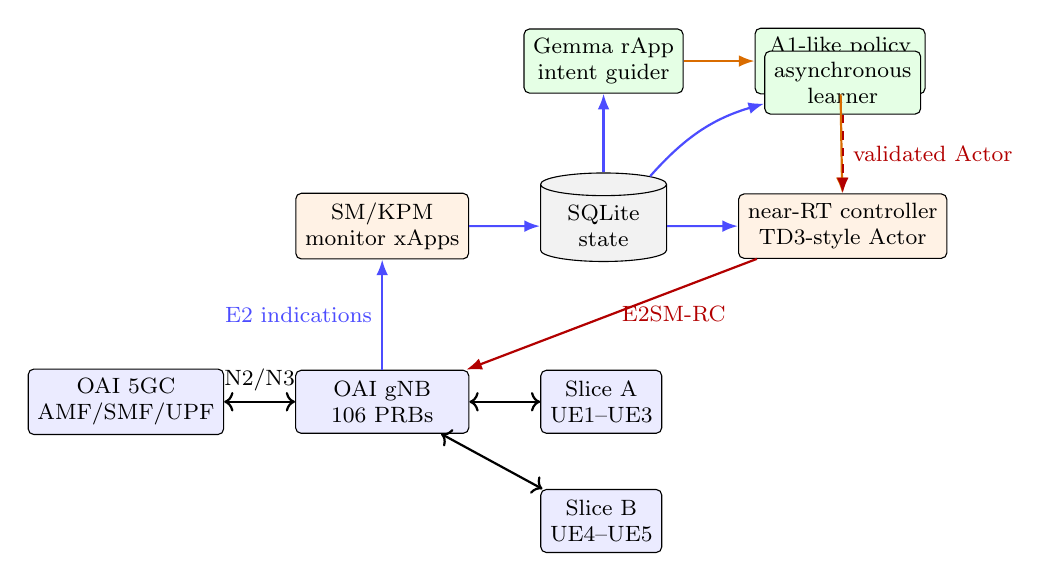
\begin{tikzpicture}[
  font=\footnotesize,
  node distance=7mm and 9mm,
  block/.style={draw,rounded corners=2pt,minimum height=8mm,align=center,fill=white},
  ran/.style={block,fill=blue!8}, ric/.style={block,fill=orange!10},
  app/.style={block,fill=green!10}, db/.style={cylinder,shape border rotate=90,draw,aspect=0.25,minimum height=11mm,minimum width=16mm,fill=gray!10,align=center},
  measure/.style={-{Latex[length=2mm]},thick,blue!70},
  guide/.style={-{Latex[length=2mm]},thick,orange!85!black},
  control/.style={-{Latex[length=2mm]},thick,red!70!black}
]
\node[ran] (core) {OAI 5GC\\AMF/SMF/UPF};
\node[ran,right=of core,minimum width=22mm] (gnb) {OAI gNB\\106 PRBs};
\node[ran,right=of gnb] (uesa) {Slice A\\UE1--UE3};
\node[ran,below=of uesa] (uesb) {Slice B\\UE4--UE5};

\node[ric,above=14mm of gnb] (monitor) {SM/KPM\\monitor xApps};
\node[db,right=of monitor] (db) {SQLite\\state};
\node[ric,right=of db] (ctrl) {near-RT controller\\TD3-style Actor};
\node[app,above=10mm of db] (rapp) {Gemma rApp\\intent guider};
\node[app,right=of rapp] (a1) {A1-like policy\\HTTP/SQLite};
\node[app,above=10mm of ctrl] (learner) {asynchronous\\learner};

\draw[measure] (gnb) -- node[left]{E2 indications} (monitor);
\draw[measure] (monitor) -- (db);
\draw[measure] (db) -- (rapp);
\draw[measure] (db) -- (ctrl);
\draw[measure,bend left=16] (db) to (learner);
\draw[guide] (rapp) -- (a1);
\draw[guide] (a1) -- (ctrl);
\draw[control] (ctrl) -- node[right]{E2SM-RC} (gnb);
\draw[control,dashed] (learner) -- node[right]{validated Actor} (ctrl);
\draw[<->,thick] (core) -- node[above]{N2/N3} (gnb);
\draw[<->,thick] (gnb) -- (uesa);
\draw[<->,thick] (gnb) -- (uesb);
\end{tikzpicture}

  \caption{Deployed LLM-hRIC network-slicing architecture. Solid blue arrows carry measurements and state, orange arrows carry guidance, and red arrows carry near-RT PRB controls. The RAN scheduler runs independently of all RIC clocks.}
  \label{fig:architecture}
\end{figure*}

\begin{table}[t]
\centering
\caption{Five-UE slice configuration.}
\label{tab:ue-map}
\begin{tabular}{llll}
\toprule
Slice & S-NSSAI & UEs & DNN \\
\midrule
A & \snssaiA & UE1--UE3 & \texttt{oai} \\
B & \snssaiB & UE4--UE5 & \texttt{openairinterface} \\
\bottomrule
\end{tabular}
\end{table}

\subsection{Intent and constrained objective}
\label{subsec:objective}
The campaign uses two natural-language intents that differ only by exchanging the two slices. Each contains a single templated field, the calibrated floor $F$:
\begin{itemize}
  \item \emph{Intent~1}: ``Maximize total DL throughput, prioritize slice \snssaiA, and keep aggregate DL throughput of slice \snssaiB{} at or above $F$ Mbps.''
  \item \emph{Intent~2}: the same sentence with the two slices exchanged.
\end{itemize}
An intent therefore identifies a \emph{priority slice}, whose throughput should be increased, and a \emph{protected slice}, whose aggregate downlink throughput must remain above $F$. For slice throughputs $T_A$ and $T_B$, the controller first seeks $T_{\mathrm{protected}}\geq F$ and only then maximizes total and priority-slice throughput; the near-RT reward realizes that ordering as a two-branch function that withholds all throughput utility on a violated step, and is stated in full with its weights in the deployment section.

Three details of the objective are prototype-specific and must not be read as generic O-RAN semantics. First, $F$ is not a contractual service-level agreement (SLA). It is derived per seed and per testbed during calibration as $F=0.90\,p_{10}$, where $p_{10}$ is the nearest-rank tenth percentile of the protected slice's measured downlink throughput at that intent's reference allocation (65\% Slice-A PRBs for Intent~1, 35\% for Intent~2); the resulting value is rendered into the intent sentence with two decimals. It is thus a testbed-feasible target with a 10\% margin below an already pessimistic observed level.

Second, the priority requirement is quantitative but does \emph{not} appear in the sentence. A minimum commanded priority-slice PRB ratio of $\rho_{\min}=55\%$ is fixed by the campaign runner, embedded in each calibrated policy, and published as a machine-readable policy-constraint field alongside the intent text. The controller reads it from that field; the regular-expression fallback that would parse it out of the sentence finds nothing for these two intents and would yield zero. Consequently the paper distinguishes throughout between \emph{SLA satisfaction} ($T_{\mathrm{protected}}\geq F$) and \emph{intent satisfaction} (SLA satisfaction \emph{and} a commanded priority ratio of at least $\rho_{\min}$), and the two rates differ substantially in the results.

Third, the identities of the priority and protected slices are resolved from the same machine-readable policy context, with regular-expression parsing of the intent sentence only as a fallback; if neither resolves, the protected slice silently defaults to the last slice in the catalogue. In the reported campaign both identities are always supplied explicitly by calibration, so the fallback path is never exercised.

\subsection{Action space and feasible interval}
The near-RT action is a single scalar in $[0,1]$, issued every 100~ms. It is interpolated over a feasible interval of admissible Slice-A budgets and rounded to an integer number of PRBs; the complementary budget of the other slice is the remainder of the 106-PRB cell, and the two budgets are emitted as complementary percentage ratios in the E2 control message. The feasible interval is recomputed for every action from the percentage bounds then active, with ceiling on minima, floor on maxima, and a complementarity constraint so that the same split is admissible for both slices; an empty interval is a hard error rather than a clipped action. Section~\ref{subsec:ctl-state} states the rounding rule, the interval construction and the resulting integer endpoints in full, and that derivation is not repeated here.

Two bound sources are combined. Every arm is confined to a fixed \emph{operational envelope} of 10--90\% per slice, which is a campaign-specification constant applied before any run and not a calibration output; because the endpoints are taken inward to integer PRBs, the realized envelope is slightly narrower than 10--90\%. In addition, calibration derives per-intent \emph{policy-constraint bounds} from the fixed-ratio sweep and publishes them with the A1 policy. A swept allocation is counted as safe only if it satisfies \emph{both} conditions: the protected slice's tenth-percentile throughput at that allocation meets $F$, \emph{and} the allocation respects the intent direction, that is at least 55\% for Intent~1 and at most 45\% for Intent~2. Intent~1 then publishes Slice~A between 55\% and the largest safe allocation, and Intent~2 between the smallest safe allocation and 45\%. Only the arms that read guidance intersect these bounds with the operational envelope; the unguided arm sees the operational envelope alone.

The division of labour between the language model and the guardrail is worth stating precisely, because it is easy to overstate the model's authority. The bounds carried by the A1 policy are \emph{not} the model's own. The rApp projects the model's proposed ratio into the calibrated policy-constraint bounds and then replaces the model's bound proposal with those calibrated bounds before publication. The guardrail is therefore calibration-derived and deterministic; the language model contributes the target \emph{inside} it, and the near-RT controller sees only the projected target and the calibrated interval.

\subsection{Traffic scenarios}
The campaign keeps the aggregate offered load at 150~Mbps in every phase of every scenario and changes only its distribution across UEs; the per-UE rates are listed in Table~\ref{tab:traffic}. Consequently \emph{balanced} means equal per-UE demand, not equal slice totals: its Slice-A/Slice-B offered loads are 90/60~Mbps because the slices contain three and two UEs.

Section~\ref{sec:methodology} describes the traffic generator, the shaper that realizes the phase pattern of a dynamic scenario, and the per-segment fidelity audit. One consequence must be stated here, because it bounds what the pilot shows: the balanced scenario has a single phase and therefore installs no shaper, so its reported segment success rate is vacuous and is not evidence of shaper fidelity. That evidence can only come from the two dynamic scenarios, which remain to be run.

\begin{table}[t]
\centering
\caption{Per-UE offered downlink traffic (Mbps). Phases alternate every 5~s; the balanced scenario has a single phase.}
\label{tab:traffic}
\begin{tabular}{lcccc}
\toprule
& \multicolumn{2}{c}{Phase 1} & \multicolumn{2}{c}{Phase 2}\\
Scenario & A & B & A & B\\
\midrule
Balanced & 30 & 30 & --- & ---\\
Slice-A-heavy & 36 & 21 & 44 & 9\\
Slice-B-heavy & 28 & 33 & 12 & 57\\
\bottomrule
\end{tabular}
\end{table}

\section{Slicing Control Path in OAI and FlexRIC}
\label{sec:oai}
This section documents the source changes that make a stock OAI/FlexRIC installation slice-controllable, so that the deployment can be reproduced. Relative to the OAI base revision, the working tree contains nine modified source and configuration files plus the FlexRIC submodule pointer, and four added files; the nine modified files account for +329/$-$71 lines. The FlexRIC submodule, base revision \texttt{340c36bc}, contains eleven modified files (+476/$-$228 lines) plus two added directories, the C slice-control xApp and the \systemname{} Python package. No file in the FlexRIC RC service-model encoder was touched: the new control action rides on the unmodified RC service model, and only the gNB-side RAN function and the xApp that drives it are new; the action semantics under Style~2 / Action~6 are nevertheless locally defined (Section~\ref{sec:limitations}). Table~\ref{tab:oai-mods} enumerates the complete surface.

\subsection{Modification surface}
The changes fall into six groups. The gNB RAN function gains a second E2SM-RC CONTROL style and its decoder. The gNB MAC gains a slice-aware downlink resource-block allocator and the policy table it reads. The RFSimulator change is a build-portability fix only. The configuration files add the second S-NSSAI and the E2 agent block. On the RIC side, a new C xApp actuates PRB policies and the existing monitor xApps were extended; the FlexRIC library changes are reliability fixes described in Section~\ref{subsec:oai-reliability}.

\begin{table*}[t]
\centering
\caption{Complete modification surface. OAI paths are relative to the repository root; FlexRIC paths are relative to \texttt{openair2/E2AP/flexric}. ``new'' marks files that do not exist upstream; otherwise inserted/deleted line counts are given.}
\label{tab:oai-mods}
\scriptsize
\begin{tabular}{@{}llp{0.50\textwidth}@{}}
\toprule
File & Change & Role \\
\midrule
\multicolumn{3}{@{}l}{\emph{gNB RAN function (RC service model)} --- \texttt{openair2/E2AP/RAN\_FUNCTION/}}\\
\texttt{O-RAN/rc\_ctrl\_service\_style\_2.c} & new (216 lines) & Style~2 RAN-function definition and RRM Policy Ratio List decoder \\
\texttt{O-RAN/rc\_ctrl\_service\_style\_2.h} & new (37 lines) & control-action and RAN-parameter identifier enumerations \\
\texttt{O-RAN/ran\_func\_rc.c} & +22/$-$4 & advertises two CONTROL styles; dispatches Style~2 / Action~6; logs style and action \\
\texttt{CMakeLists.txt} & +2 & adds the decoder to \texttt{e2\_ran\_func\_cuup} and \texttt{e2\_ran\_func\_du\_cucp\_cuup} \\
\midrule
\multicolumn{3}{@{}l}{\emph{gNB MAC downlink scheduler} --- \texttt{openair2/LAYER2/NR\_MAC\_gNB/}}\\
\texttt{gNB\_scheduler\_dlsch\_default\_policies.c} & +203/$-$47 & splits proportional fair into a retransmission/MAC-CE pass and new-data passes; adds the budgeted per-slice pass, the policy installer and PRB accounting \\
\texttt{gNB\_scheduler\_dlsch\_default\_policies.h} & +2 & exports \texttt{nr\_dl\_slice\_prb\_policy()} and \texttt{nr\_mac\_set\_dl\_slice\_policies()} \\
\texttt{nr\_mac\_gNB.h} & +15 & \texttt{nr\_dl\_slice\_policy\_t} and five per-MAC policy/accounting fields \\
\texttt{main.c} & +2/$-$1 & default \texttt{dl\_rb\_alloc} hook becomes \texttt{nr\_dl\_slice\_prb\_policy} \\
\midrule
\multicolumn{3}{@{}l}{\emph{Radio simulator} --- \texttt{radio/rfsimulator/}}\\
\texttt{simulator.cpp} & +74/$-$15 & option table rebuilt with helper functions for the C++ toolchain; no functional change \\
\midrule
\multicolumn{3}{@{}l}{\emph{Testbed configuration} --- \texttt{ci-scripts/conf\_files/}}\\
\texttt{gnb.sa.band78.106prb.rfsim.conf} & +8/$-$3 & second S-NSSAI in \texttt{snssaiList}; \texttt{e2\_agent} block; local N2/N3 address \\
\texttt{nrue.uicc.conf} & +1/$-$1 & explicit PDU-session id, DNN \texttt{oai} and SD \texttt{0xFFFFFF} \\
\texttt{nrue.uicc.slice2.conf} & new & single UE on Slice~B (IMSI \texttt{208990100001101}, DNN \texttt{openairinterface}) \\
\texttt{nrue.uicc.2slice.conf} & new & two UEs, one per slice, with an AWGN channel-model block \\
\midrule
\multicolumn{3}{@{}l}{\emph{FlexRIC xApps} --- \texttt{examples/xApp/}}\\
\texttt{c/rc\_slice\_ctrl/xapp\_rc\_slice\_ctrl.c} & new (573 lines) & JSON policy parser, E2SM-RC message encoder, Unix-socket actuator server \\
\texttt{c/rc\_slice\_ctrl/CMakeLists.txt} & new & \texttt{xapp\_rc\_slice\_ctrl} target linked against \texttt{e42\_xapp} \\
\texttt{c/CMakeLists.txt} & +1/$-$1 & registers the new sub-directory \\
\texttt{c/monitor/xapp\_kpm\_moni.c} & +135/$-$15 & KPM record bounds checks, collection-timestamp normalization, SQLite sink \\
\texttt{c/monitor/CMakeLists.txt} & +1 & links \texttt{-lsqlite3} \\
\texttt{python3/xapp\_mac\_rlc\_pdcp\_gtp\_moni.py} & +234/$-$161 & four service-model subscriptions, RIC-side sampling throttle, per-callback exception isolation, database writer \\
\midrule
\multicolumn{3}{@{}l}{\emph{FlexRIC library (reliability)} --- \texttt{src/}}\\
\texttt{lib/msg\_hand/reg\_e2\_nodes.c} & +13/$-$3 & duplicate E2 SETUP replaces the stale registry entry instead of aborting \\
\texttt{sm/pdcp\_sm/ie/pdcp\_data\_ie.c} & +8/$-$6 & removes the four counter-ordering assertions executed inside the gNB SM plugin \\
\texttt{xApp/sync\_ui.c}, \texttt{xApp/sync\_ui.h} & +18/$-$11 & adds \texttt{prepare\_sync\_ui()}; the bounded wait returns a status instead of asserting \\
\texttt{xApp/e42\_xapp.c} & +31/$-$4 & resets the synchronization flags before every send; handles timeout at three call sites \\
\texttt{xApp/msg\_handler\_xapp.c} & +13/$-$21 & ignores late CONTROL ACK/FAILURE; removes the redundant CONTROL pending-event timer \\
\texttt{xApp/db/sqlite3/sqlite3\_wrapper.c} & +22/$-$6 & 32-bit RLC byte constraint removed; bounded insert retry; busy timeout \\
\bottomrule
\end{tabular}
\end{table*}

\subsection{E2SM-RC slice control action}
The RAN function is the FlexRIC RC service model (\texttt{ORAN-E2SM-RC}, OID \texttt{1.3.6.1.4.1.53148.1.1.2.3}, service-model identifier~3, revision~1), encoded in ASN.1/PER. \texttt{fill\_rc\_control()} in \texttt{ran\_func\_rc.c} now declares two CONTROL styles instead of one. Style~1 (\emph{Radio Bearer Control}) is unchanged; \texttt{fill\_rc\_ctrl\_style\_2()} adds Style~2, \emph{Radio Resource Allocation Control}, with header format~1, message format~1, outcome format~1, no call-process identifier, no control outcome parameters, and a single control action: identifier~6, \emph{Slice-level PRB quota}, with one associated RAN parameter, \emph{RRM Policy Ratio List}. The style is advertised by the monolithic gNB and CU definitions; the DU-only and CU-UP-only definitions advertise no RC services and are unaffected.

The control message reproduces the E2SM-RC RRM Policy Ratio List hierarchy using RAN Parameter IDs 1--12 (Table~\ref{tab:oai-ranparam}). Each list element is an RRM Policy Ratio Group of exactly four parameters: an RRM Policy structure (ID~3) containing an RRM Policy Member List (ID~4) whose member carries PLMN Identity (ID~6) and S-NSSAI (ID~7, carrying SST at ID~8 and an optional SD at ID~9), followed by Min (ID~10), Max (ID~11) and Dedicated (ID~12) PRB Policy Ratio integers. Two deviations must be stated. First, the PLMN Identity element is required to be present---the member structure must contain exactly two parameters---but the gNB never dereferences it and never checks its identifier, so PLMN is transported and ignored in this prototype. Second, SST and SD are transported as ASCII-text OCTET STRINGs (for example \texttt{"1"} and \texttt{"0xffffff"}, converted with \texttt{strtoul} base~0) or as plain INTEGERs, rather than the 3GPP binary octet encoding; an absent SD defaults to \texttt{0xffffff}.

\begin{table}[t]
\centering
\caption{RAN parameters of the Slice-level PRB quota control message.}
\label{tab:oai-ranparam}
\scriptsize
\begin{tabular}{@{}cll@{}}
\toprule
ID & RAN parameter & Decoder expectation \\
\midrule
1 & RRM Policy Ratio List & LIST, $\leq$ 1024 elements \\
2 & RRM Policy Ratio Group & STRUCT of 4 (size only) \\
3 & RRM Policy & STRUCT of 1 \\
4 & RRM Policy Member List & LIST, element 0 used \\
5 & RRM Policy Member & STRUCT of 2 (size only) \\
6 & PLMN Identity & present but not read \\
7 & S-NSSAI & STRUCT of 1 or 2 \\
8 & SST & text/INTEGER, $\leq 255$ \\
9 & SD & text/INTEGER, $\leq$ \texttt{0xffffff} \\
10 & Min PRB Policy Ratio & INTEGER, 0--100 \\
11 & Max PRB Policy Ratio & INTEGER, 0--100 \\
12 & Dedicated PRB Policy Ratio & INTEGER, 0--100 \\
\bottomrule
\end{tabular}
\end{table}

Dispatch happens in \texttt{write\_ctrl\_rc\_sm()}. Every CONTROL logs its style and action, and a message with style~2 and action~6 is handed to \texttt{apply\_rc\_ctrl\_style\_2\_slice\_level\_prb\_quota()}. The Control Header still carries a UE identifier, which the gNB ignores for this action because the policy is cell-wide. The decoder validates, in order: exactly one top-level RAN parameter, whose identifier is~1 and whose value is a non-null LIST of at most \texttt{MAX\_NUM\_SLICES}~=~1024 elements; per group, a structure of exactly four parameters, an RRM Policy structure with exactly one sub-parameter, a member list with at least one member, a member structure of exactly two parameters, an S-NSSAI structure of one or two parameters, $\mathrm{SST}\leq255$ and $\mathrm{SD}\leq\texttt{0xffffff}$, and the ratio chain $0\leq r_{\min}\leq r_{\mathrm{dedicated}}\leq r_{\max}\leq100$. Every check is an \texttt{AssertError}, which is not compiled out in release builds: it prints the failed condition with function, file and line to standard error and returns failure, so each rejection is observable.

Atomicity is obtained by construction. The decoder parses the whole message into a local \texttt{nr\_dl\_slice\_policy\_t} array and calls \texttt{nr\_mac\_set\_dl\_slice\_policies()} only after every group has been accepted; a malformed message therefore never reaches MAC state. The installer re-checks the same ratio bounds and writes the policy table, its length and its enable flag while holding \texttt{gNB\_MAC\_INST::sched\_lock}---the same mutex that \texttt{gNB\_dlsch\_ulsch\_scheduler()} holds for the whole duration of a slot---so no scheduling opportunity ever observes a partially applied policy set. One honest caveat: the installer clears the table before its own re-validation loop and does not roll back on a mid-loop rejection; this path is unreachable in practice because the decoder applies identical bounds first. A further limitation is that the RIC Control Acknowledge is returned with a success outcome even when the application fails; rejection is visible only as an error line in the gNB log, not in the E2 outcome.

\subsection{S-NSSAI-aware downlink scheduler}
The scheduler hook is the existing \texttt{dl\_rb\_alloc} function pointer, invoked as step~6 of \texttt{nr\_dl\_schedule()} after candidate collection, rank/precoding selection, beam selection, time-domain allocation and MCS selection, and before transport-block-size computation and DCI/PUCCH allocation. \texttt{mac\_top\_init\_gNB()} now installs \texttt{nr\_dl\_slice\_prb\_policy} instead of \texttt{nr\_dl\_proportional\_fair} as the default allocator; the \texttt{phy\_test} branch is untouched. When no policy is installed, \texttt{nr\_dl\_slice\_prb\_policy()} delegates directly to \texttt{nr\_dl\_proportional\_fair()}, which was refactored but is behaviorally identical to upstream, so an unconfigured build matches stock OAI.

With policies installed, allocation proceeds in four ordered passes over one proportional-fair ordering of the candidates: (1) HARQ retransmissions, each at its exact stored resource-block count; (2) UEs with no pending data that need five resource blocks for a timing-advance command or a beam-switch MAC control element; (3) for each configured policy in table order, new-data candidates of that S-NSSAI in proportional-fair order, capped at $\lfloor N_{\mathrm{RB}}\, r_{\mathrm{dedicated}}/100 \rfloor$ resource blocks in total; and (4) new-data candidates matching no policy, uncapped. Passes~1 and~2 are the stock proportional-fair phases with an added guard so that no candidate is allocated twice across the new multi-pass structure. Slice budgets can therefore never displace retransmissions or MAC control elements, and only new-data resource blocks are charged against a budget.

A UE is matched by the S-NSSAI of its first data radio bearer. The MAC caches that S-NSSAI per logical channel in \texttt{nr\_lc\_config\_t::nssai}, written from the F1AP DRB-to-be-setup, which the RRC copies from the NGAP PDU Session Resource Setup S-NSSAI; \texttt{collect\_dl\_candidates()} scans the logical-channel configuration, takes the S-NSSAI of every channel with \texttt{lcid}~$\geq$~4, and copies it into the scheduling candidate. Lookup is exact equality on both SST and the 24-bit SD, with no wildcard or partial match. A UE with no DRB defaults to SST~0 / SD~\texttt{0xffffff} and therefore never matches a policy, falling through to pass~4. For a UE with several DRBs on different slices the scan retains the S-NSSAI of the first DRB reporting a non-zero 5QI, otherwise of the last DRB; this is unambiguous in the present testbed because every UE has exactly one PDU session and one DRB.

The per-slot budget denominator is the full cell bandwidth, that is the number of schedulable resource blocks passed by the preprocessor (\texttt{carrierBandwidth}~=~106 here), not what remains after retransmissions. Retransmission resource blocks lie outside the budget but do reduce the free blocks the budgeted pass can find. With the 80/20 split of the sample policy the per-slot new-data caps are $\lfloor 106\cdot 80/100\rfloor=84$ and $\lfloor 106\cdot 20/100\rfloor=21$ resource blocks, one block being lost to integer truncation. Within a pass, each UE receives at most one contiguous block: the budget caps the largest free run found for that candidate's symbol bitmap, with a five-resource-block minimum, so fragmentation can leave part of a budget unusable. Three further mechanisms bound the outcome and should be stated: a policy with a zero dedicated ratio is skipped entirely and its UEs are excluded from pass~4 as well, receiving no new-data grants; the budget sums the available resource blocks over all beams while the allocator is invoked once per beam group, which is exact only for the single-beam configuration used here; and the downlink control-channel limit caps the testbed at four scheduled UEs per slot out of five, so a pass can terminate early and the loop simply proceeds to the next policy. The MAC also maintains a cumulative per-policy resource-block counter, reset on every policy installation, and emits one \texttt{slice\_prb} log line per active policy every 100 frames on slot~0; this is the gNB-side ground truth for realized PRB share.

\begin{figure}[t]
  \centering
  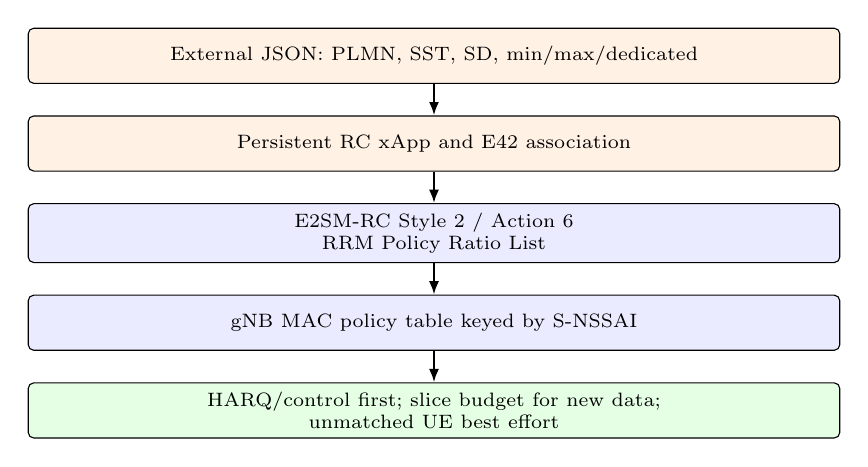
\begin{tikzpicture}[font=\scriptsize,node distance=4mm,
 box/.style={draw,rounded corners=2pt,align=center,minimum width=.85\columnwidth,minimum height=7mm},
 arrow/.style={-{Latex[length=1.7mm]},thick}]
\node[box,fill=orange!10] (json) {External JSON: PLMN, SST, SD, min/max/dedicated};
\node[box,fill=orange!10,below=of json] (xapp) {Persistent RC xApp and E42 association};
\node[box,fill=blue!8,below=of xapp] (rc) {E2SM-RC Style 2 / Action 6\\RRM Policy Ratio List};
\node[box,fill=blue!8,below=of rc] (mac) {gNB MAC policy table keyed by S-NSSAI};
\node[box,fill=green!10,below=of mac] (sched) {HARQ/control first; slice budget for new data;\\unmatched UE best effort};
\draw[arrow] (json)--(xapp);
\draw[arrow] (xapp)--(rc);
\draw[arrow] (rc)--(mac);
\draw[arrow] (mac)--(sched);
\end{tikzpicture}

  \caption{Policy translation from external JSON to the OAI downlink scheduler.}
  \label{fig:oai-path}
\end{figure}

\subsection{Persistent RC actuator}
Fig.~\ref{fig:oai-path} traces one policy from the external JSON document written by the near-RT controller, through the persistent xApp and the E2SM-RC control message, to the per-slot budget applied by the gNB downlink scheduler. The C RC xApp no longer embeds the two S-NSSAIs. It reads an external JSON document (Table~\ref{tab:oai-json}) whose top-level \texttt{policies} array contains one object per slice with six mandatory keys: \texttt{plmn} (5--6 ASCII digits), \texttt{sst} and \texttt{sd} (string or integer, bounded by 255 and \texttt{0xffffff}), and \texttt{min\_prb}, \texttt{max\_prb}, \texttt{dedicated\_prb} (integers in $[0,100]$). It enforces $r_{\min}\leq r_{\mathrm{dedicated}}\leq r_{\max}$ per policy and a running sum of dedicated ratios of at most 100 across policies. The Python controller writes the same document atomically (temporary file, \texttt{fsync}, \texttt{rename}) and revalidates it against the identical rules before every action.

\begin{table}[t]
\caption{External PRB policy document consumed by the RC actuator.}
\label{tab:oai-json}
\scriptsize
\begin{verbatim}
{"policies": [
 {"plmn": "20899", "sst": 1, "sd": "0xffffff",
  "min_prb": 0, "max_prb": 100, "dedicated_prb": 80},
 {"plmn": "20899", "sst": 1, "sd": "0x123456",
  "min_prb": 0, "max_prb": 100, "dedicated_prb": 20}]}
\end{verbatim}
\end{table}

The xApp runs either one-shot (\texttt{--policy-file}, \texttt{--once}) or as a persistent server (\texttt{--serve}) bound to an \texttt{AF\_UNIX} stream socket. A persistent association is required because a one-shot invocation must, per action, load every service-model plugin, create a fresh per-process SQLite database, open an SCTP association, complete the E42 SETUP exchange and observe a fixed one-second settling delay before it may send---well over one second, against a 100~ms control period, and leaking one database file per action. The persistent mode pays that cost once. The request is a single newline-terminated JSON line carrying only \texttt{request\_id} and \texttt{policy\_file}; the policy content is not sent over the socket, and the server re-reads the file from disk on every request. The response is one JSON line containing the echoed request identifier, a success flag, and two \texttt{CLOCK\_REALTIME} timestamps, \texttt{sent\_ts\_ms} taken before the file is loaded and \texttt{response\_ts\_ms} taken after the last CONTROL acknowledgement. The controller uses \texttt{response\_ts\_ms} to anchor the effect-observation window; the RC latency reported in this paper is the client-side socket round trip measured in the Python controller, not a value returned by the xApp.

Three operational properties follow from the implementation and are stated for reproducibility. First, the actuator resolves the set of connected E2 nodes and each node's RC RAN-function identifier once at start-up and refuses to start if no node is attached; nodes that attach later are never controlled, so the gNB must be running before the actuator is launched. Second, RIC request identifiers are drawn from a monotonically increasing registry that never recycles keys and are asserted to fit in 16 bits, so one actuator process supports at most 65\,536 CONTROL procedures, about 109~minutes at the 100~ms period; the reported runs are approximately 87~minutes, and the experiment runner restarts the actuator per run. Third, the accept loop is sequential with no per-connection receive timeout, and the client socket timeout (5~s) is shorter than the effective E2 CONTROL deadline (approximately 6~s), so a CONTROL timeout would leave the server writing to a closed socket with no \texttt{SIGPIPE} handler installed. Neither condition occurred in the reported runs, in which every action was acknowledged.

\subsection{Long-run reliability fixes}
\label{subsec:oai-reliability}
Four defects in stock FlexRIC aborted a process during multi-hour, high-rate operation. Each was fixed at its root cause rather than by retry logic in the experiment scripts.

\begin{description}
\item[Duplicate E2 node registration.] A second E2 SETUP carrying an already-registered global E2 node identifier---after a gNB restart, an SCTP reconnect, or a setup arriving before the stale entry was reaped---tripped an assertion in the node registry and aborted the near-RT RIC, taking every xApp association with it. The registry now extracts and frees the stale RAN-function/component-configuration entry, logs the replacement, and re-registers the node.
\item[PDCP counter snapshot.] The PDCP service model treated the orderings $\mathrm{pkts}\leq\mathrm{bytes}$ on four transmit/receive counter pairs as fatal invariants. Packet and byte counters are updated independently by the PDCP data path, so a snapshot can carry the new packet count with the previous byte count, and the 32-bit byte counters wrap before their packet counterparts. Because this check executes inside the gNB's service-model agent plugin, sustained five-UE traffic aborted the RAN itself. The invariant was removed; consumers compute deltas and discard reset and wrap samples. The launcher enforces the fix at start-up: it scans the resolved \texttt{libpdcp\_sm.so} for the four assertion strings, refuses to start if any is present, and records the plugin's absolute path and SHA-256 digest.
\item[E42 synchronization.] Three distinct defects were corrected. The synchronization flags were previously cleared inside the wait function, after the request had already been written to the socket, so an acknowledgement arriving in that window was discarded and the caller blocked until timeout; the reset was hoisted into a separate \texttt{prepare\_sync\_ui()} step executed before every subscription, subscription-delete and control send. A timeout was a fatal assertion; the wait now returns a status, and each of the three call sites logs, releases the active procedure and reports failure. An acknowledgement whose request identifier had already been released aborted the xApp; late CONTROL acknowledgements and failures are now ignored. In addition, the synchronous CONTROL path inserted a redundant ten-second timer into the pending-event map on every request, and removing an entry that had already been reaped corrupted that container after tens of thousands of control cycles; the bounded conditional wait is now the single CONTROL timeout, while the SETUP, subscription and subscription-delete pending events are unchanged.
\item[xApp database.] The FlexRIC per-process xApp database aborted the monitor in two ways. Its RLC schema bounded the cumulative SDU byte counters to 32 bits, so every insert failed with a constraint error once a run exceeded 4~GiB per bearer direction; that bound was removed. Separately, any insert error, including transient busy or locked results from concurrent readers, was a fatal assertion; inserts now retry for up to 500~ms, the connection sets a five-second busy timeout and write-ahead logging, and a genuine error prints the SQLite message and the offending statement before failing.
\end{description}

The KPM collector also received a correctness fix: measurement records were indexed by label rather than by measurement, which read past the record list for measurements declaring multiple labels. Record-list length, unknown value types and unknown UE-identity types are now bounds-checked, and the reported indication latency normalizes the collection timestamp to epoch milliseconds.

\subsection{Build configuration and reproduction}
The E2 control path is gated at compile time. \texttt{E2\_AGENT} is a cache variable defaulting to \texttt{OFF}; \texttt{./build\_oai --build-e2} sets it, which adds the E2AP subtree, builds the RAN-function libraries with the new decoder, and links and defines \texttt{E2\_AGENT} for \texttt{nr-softmodem}. The body of the slice-quota handler is compiled only when \texttt{NGRAN\_GNB\_DU} is defined, which the DU/CU-CP/CU-UP library linked into \texttt{nr-softmodem} provides; in \texttt{nr-cuup} the handler is inert and returns success with a warning. The MAC-side changes are not behind any flag, but they fall back to stock proportional fair when no policy is installed, so a build without the E2 agent is behaviorally identical to upstream OAI.

The reference host is Ubuntu 22.04 with GCC 10.5.0, CMake 3.22.1 and Ninja. The RAN is built with \texttt{./build\_oai -I --gNB --nrUE --build-e2 --ninja}; subsequent rebuilds additionally require \texttt{ninja -C cmake\_targets/ran\_build/build nr-softmodem nr-uesoftmodem params\_libconfig rfsimulator}, because the softmodems load the configuration and radio libraries at run time and would otherwise start and exit before reading their configuration. FlexRIC is configured with \texttt{cmake -S . -B build -DXAPP\_MULTILANGUAGE=ON} and built with targets \texttt{nearRT-RIC}, \texttt{xapp\_rc\_slice\_ctrl}, \texttt{xapp\_kpm\_moni}, \texttt{pdcp\_sm} and \texttt{xapp\_sdk}. The multilanguage option is off by default upstream but is mandatory here: without it the SWIG bindings are not generated and the Python monitor xApp, which the launcher hard-requires, cannot run. The pinned encoding configuration is E2AP~v2, KPM~v2.03, with the RC and KPM service models ASN.1-encoded and the MAC, RLC, PDCP and GTP service models using the plain FlexRIC encoding.

One further change is required to build the reference testbed at all: \texttt{radio/rfsimulator/simulator.cpp} is compiled as C++, and the designated-initializer parameter macros used for the RFSimulator option table are not accepted by GCC~10. The option table was rewritten using seven small helper functions that construct each parameter descriptor by value. All fifteen parameter names, flags, target pointers and default values are unchanged, and the rewrite has no run-time effect; it is a build-portability fix, not a system feature.

The gNB uses PLMN 208/99, band~78, 106 PRB at 30~kHz subcarrier spacing, and its only slicing-related change is the second entry in \texttt{snssaiList}. Two non-slicing changes matter to a reproducer: the appended \texttt{e2\_agent} block, which points the agent at a near-RT RIC on \texttt{127.0.0.1} and at a service-model directory that the launcher overrides at run time with \texttt{--e2\_agent.sm\_dir}, and the local N2/N3 address, set to \texttt{192.168.71.129} with the AMF at \texttt{192.168.71.132}. The five UE configurations of the reported runs are not the checked-in files: they are generated at launch by the experiment script into a per-run directory as \texttt{nrue.uicc.ue1.conf} through \texttt{nrue.uicc.ue5.conf}, with IMSIs \texttt{208990100001100}--\texttt{208990100001104}, DNN \texttt{oai} and SD \texttt{0xFFFFFF} for UE1--UE3 and DNN \texttt{openairinterface} and SD \texttt{0x123456} for UE4--UE5. Each UE runs in its own network namespace against its own RFSimulator server address. The checked-in \texttt{nrue.uicc.slice2.conf} and \texttt{nrue.uicc.2slice.conf} are single- and dual-UE convenience configurations and are not used by the five-UE campaign.

\subsection{Site adaptation and distribution}
The artifact is configured for the reference host and does not relocate itself. A reproducer must edit the following before a first run. In \texttt{config.yaml}: \texttt{control.rc\_xapp}, an absolute path into the FlexRIC build tree, and \texttt{rfsim\_channel.netns\_python}, an absolute interpreter path, both of which begin with the reference home directory; the working paths \texttt{db\_path}, \texttt{control.policy\_file}, \texttt{control.actuator\_socket}, \texttt{monitor.gnb\_log}, \texttt{monitor.nrue\_log\_dir}, the DDPG \texttt{checkpoint} and the actor \texttt{snapshot\_dir}, all of which are under \texttt{/tmp/llm\_hric}; and the traffic addresses \texttt{traffic.ext\_dn\_ip} (\texttt{192.168.72.135}) and \texttt{traffic.route\_gateway} (\texttt{192.168.72.134}), which must match the deployed core network. In the gNB configuration, the local N2/N3 address and the AMF address must match the core as well. One of these is not a portability detail but a correctness requirement: the campaign results directory must be given a persistent path. The pilot reported here wrote its results under \texttt{/tmp}, and the raw databases and trained checkpoints were destroyed when the host was rebooted to repair an unrelated GPU driver fault, because that directory does not survive a reboot.

Distribution requires one clarification. The base revisions pinned above identify the upstream OAI and FlexRIC trees that were modified, but the two added directories---the C slice-control xApp and the \systemname{} Python package---are new source that is not obtainable from either pinned revision. The release therefore consists of the pinned base revisions, a patch series over them reproducing the modified files enumerated in Table~\ref{tab:oai-mods}, and the two added directories shipped in full.
% TODO(authors): confirm the final distribution form (public fork versus patch
% series plus source drop) and set \codeurl accordingly.

\subsection{Semantics and conformance boundary}
Three semantic restrictions of this implementation should be read together with the results. First, the scheduler enforces the dedicated ratio only: although minimum and maximum ratios are validated and stored at the E2 boundary, they are not independent scheduler mechanisms, and the near-RT controller performs bound projection before transmission. Second, unused budget of one controlled slice is not reclaimed by another controlled slice; unmatched UEs consume whatever remains in the final uncapped pass. Evaluating the commanded ratio therefore requires saturating traffic on both slices. Third, the per-slice budget is a per-slot new-data cap expressed against the full cell bandwidth, not a guaranteed share.

S-NSSAI, DNN, registration and PDU-session procedures use the existing 3GPP mechanisms~\cite{3gpp23501}; no NAS, NGAP, RRC or PHY message is redefined, and the S-NSSAI the scheduler matches on is the one the core signaled for the UE's data radio bearer. The control encoding reuses the stock E2SM-RC ASN.1/PER encoder and reproduces the RRM Policy Ratio List parameter hierarchy under Control Style~2 / Action~6~\cite{oran_e2sm_rc}. The action semantics are nevertheless added locally to the OAI RC RAN function, the S-NSSAI fields deviate from the 3GPP binary encoding, the PLMN identity is not interpreted, control outcomes do not report application failures, and the system has not undergone O-RAN conformance certification. The per-slice PRB budget itself is an implementation-specific gNB scheduling policy. Section~\ref{sec:limitations} enumerates these deviations together with the measurement and evaluation limitations.

% The deployment section is split across two files: 04a opens the section and
% covers the data and guidance paths; 04b continues with control and learning.
% Their order is mandatory (04b begins at \subsection level).
\section{\systemname{} Deployment}
The magazine paper~\cite{bao2026llmhric} established the \systemname{} tier decomposition---a non-real-time LLM rApp that reasons over slow, semantically rich summaries, and a near-real-time deep reinforcement learning xApp that acts on fast RAN state---using a transmit-power allocation use case in an IAB network, with a Llama-3.1-8B rApp and a DDPG xApp. This appendix documents what had to change to make that decomposition control \emph{PRBs across two S-NSSAIs} on a live OAI/FlexRIC stack. The tier decomposition, the guidance-conditioned action space, and the asynchronous training discipline are inherited unchanged. Everything else is new: the actuated resource is the per-slice downlink PRB budget introduced in Section~III, the guidance model is a locally served Gemma checkpoint~\cite{gemma2024} rather than a hosted Llama, and the entire observation path is rebuilt on FlexRIC~\cite{flexric2026} E2 service models because no equivalent of the simulated IAB state exists in OAI.

Seven independent clocks coexist in the deployment (Fig.~\ref{fig:timing}, Table~\ref{tab:apps}): RAN slot processing in the gNB; 10~ms E2 service-model reporting; 50~ms monitor summarization, which also sets the nominal width of a derived state window; 100~ms near-RT control; 1000~ms E2SM-KPM audit collection; 10~s rApp language inference; and a free-running asynchronous learner. Fig.~\ref{fig:timing} draws the four clocks that lie on the closed control loop---summarization, control, inference, and learning---and omits the slot, E2-reporting and audit clocks, which are not on it. None of the six RIC-side clocks gates the gNB slot loop. All of them meet in a single SQLite file (\texttt{db\_path} = \texttt{/tmp/llm\_hric/llm\_hric.sqlite3}) opened concurrently by six processes.

\subsection{Measurement and state database}
Three writers populate the measurement tables, and they are separate operating-system processes rather than threads of one collector. The first is the service-model monitor xApp, \texttt{xapp\_mac\_rlc\_pdcp\_gtp\_moni.py}, a modified version of the FlexRIC Python example; it delegates all persistence to the library class \texttt{RicSmDbWriter} in \texttt{ric\_sm\_db\_writer.py}, which performs the windowing and derivation described below under a re-entrant lock because the four service-model callbacks execute on separate SDK threads. The second is the E2SM-KPM collector \texttt{xapp\_kpm\_moni.c}, extended with a SQLite writer and linked against \texttt{-lsqlite3}. The third is the near-RT controller, whose tables are described in the following subsections. The launcher brings up the whole stack with the form used by the repository README, \texttt{UE\_MODE=multi UE\_COUNT=5 START\_LLM\_HRIC=1 START\_GRAFANA=1 DDPG\_APPLY=1 ./run\_e2e\_rfsim.sh start}. The two monitors need no flag of their own---\texttt{START\_KPM\_MONITOR} already defaults to~1---whereas \texttt{START\_LLM\_HRIC} defaults to~0, so omitting it starts the observation path but neither the A1-like server, the rApp, the near-RT controller nor the actuator, and leaves no closed loop. Independently of that flag, the KPM writer stays disabled unless the environment variable \texttt{LLM\_HRIC\_DB\_PATH} is set, which the campaign runner always does.

The monitor xApp subscribes to the FlexRIC MAC, RLC, PDCP and GTP service models at a 10~ms report interval (\texttt{monitor.subscription\_interval\_ms}, restricted by the SDK to $\{1,2,5,10\}$~ms) and admits one indication per model per 50~ms sampling window, dropping indications whose statistics list is empty. Each admitted indication is stored in a layer-specific raw table---\texttt{mac\_ue\_stats\_raw}, \texttt{rlc\_rb\_stats\_raw}, \texttt{pdcp\_rb\_stats\_raw}, \texttt{gtp\_tunnel\_stats\_raw}---carrying both the E2 source timestamp \texttt{ts\_ms}, normalised to milliseconds from the agent's \texttt{tstamp} field, and the RIC receive timestamp \texttt{recv\_ts\_ms}. The 50~ms throttle is a RIC-side observation decimation only: it does not alter the gNB slot, scheduler, PHY or MAC execution period, and the E2 subscription interval likewise controls indication reporting only.

A windowing stage keyed on MAC indication timestamps derives per-UE throughput and slice summaries. Windows are contiguous and half-open, $(t_{k-1},t_k]$, where $t_k$ is the source timestamp of the $k$-th admitted MAC indication; the configured 50~ms sampling period (\texttt{monitor.summary\_period\_ms}) sets the nominal window width and bootstraps the first window only, so realised widths are 50--60~ms rather than a fixed wall-clock grid. Each MAC indication with $t_k>t_{k-1}$ advances the window; an empty UE list is treated as a valid topology state and still advances it, so consumers observe UE departure instead of a stale last-known state. Late-arriving RLC or PDCP indications bearing the same millisecond timestamp cause the window to be re-derived in place: the derived rows at that timestamp are deleted and recomputed so that bearer counters replace the initial MAC fallback. GTP indications are stored but never trigger a flush. The slice rows of every window are pre-seeded from the configured \texttt{slice\_catalog}, so both S-NSSAIs always receive a summary row even when they carry no UE.

Downlink and uplink throughput are computed from counter differences, $R = 8\,\Delta b / (1000\,\Delta t)$~Mbit/s for $\Delta b$ bytes over $\Delta t$~ms, and selected from PDCP, RLC and MAC counters in descending priority: the first strictly positive rate wins, otherwise the first defined rate, with a final fallback of zero. Inside the MAC tier the aggregate MAC-SDU byte counter takes precedence over the transport-block counter, so the recorded provenance source is one of \texttt{pdcp}, \texttt{rlc}, \texttt{mac} or \texttt{zero} and MAC-TBS is not a separately distinguishable source. Bearer-tier rates are summed over radio bearers; each UE here has a single PDU session and therefore a single DRB. A negative counter delta invalidates that tier and additionally raises a \texttt{counter\_reset} provenance flag, which is recorded rather than used to suppress the sample. One deployment fact must be stated plainly: in the monolithic gNB used here the PDCP and GTP service models key their statistics by RRC UE identity rather than by C-RNTI, because \texttt{nr-softmodem} links the combined DU/CU-CP/CU-UP E2 RAN function and the PDCP and GTP handlers populate the identity field from \texttt{rrc\_ue\_id}, a small linear counter. Those rows can never be joined to a UE, so \texttt{pdcp\_rb\_stats\_raw} and \texttt{gtp\_tunnel\_stats\_raw} are populated but unresolvable, and the effective precedence chain reduces to RLC, then MAC-SDU, then MAC-TBS, then zero. This is a property of the stock OAI E2 agent, not of the controller.

MAC counters supply per-window PRB usage and downlink BLER. PRB usage is the delta of the cumulative allocated-RB counter \texttt{dl\_aggr\_prb}, i.e.\ a count of resource blocks in the window and not a share; the slice value is the sum of the per-UE deltas, and the PRB \emph{share} used by the controller and by the rApp prompt is formed downstream by normalising a slice's PRB delta by the cell total at the same timestamp. Slice BLER is the unweighted mean over UEs reporting a value. RLC transmit-buffer occupancy is treated as a gauge rather than a counter: the last sample per bearer in the window is summed, and the slice value is suppressed unless every active UE contributed a sample. Wideband CQI and BLER share a single validity mask requiring $0\leq\mathrm{CQI}\leq15$ and $0\leq\mathrm{BLER}\leq1$ for \emph{every} active UE in the slice; when the mask is not asserted the controller zeroes both features. We note explicitly that in the reported rfsimulator pilot the gNB reports a constant zero wideband CQI and an effectively zero BLER while the mask remains asserted, because zero is inside both admissible ranges. The mask detects absent or out-of-range reports, not degenerate constant ones, and the three channel-related state features consequently carried no information in these runs.

RNTI-to-UE/S-NSSAI bindings are discovered at runtime from the per-UE \texttt{nrUE$i$.log} files, which are the only source that ties a stable UE configuration to its current C-RNTI; the writer matches the stock OAI print \texttt{UE 0 RNTI \%04x stats} in the last 8~MiB of each log and takes the most recent occurrence. The gNB log is used solely as a consistency check against the stock \texttt{UE RNTI \%04x CU-UE-ID} print, and the map is accepted only if every configured UE yields a match, all RNTIs are distinct, and the discovered set is a subset of the RNTIs the gNB reports; otherwise the whole map is refused and the writer falls back to the static list \texttt{monitor.rnti\_slice\_map}. The design reason for preferring the UE-side log is recorded in the code: CU-UE-ID reflects attach order, not catalogue identity, so an attach-order mapping would silently mislabel slices after a UE restart. Indications whose RNTI cannot be resolved are still written to the raw tables with null \texttt{ue\_id}, \texttt{plmn}, \texttt{sst} and \texttt{sd}, and are excluded from every derived table both by an SQL predicate and by an explicit guard, so they remain auditable but are never attributed to a slice. Two deployment caveats follow. First, the gNB cross-check relies on OAI's periodic MAC statistics print, which fires only every 128 frames and which OAI permanently disables once the UE count exceeds \texttt{stats\_max\_ue} (default 8, not overridden by the deployed gNB configuration); the check is therefore live at five UEs and silently degrades to no check above eight. Second, because the PDCP and GTP models report a permanently unresolvable identity, the writer's once-per-second rediscovery path fires for the entire run, re-reading up to six log tails per second.

Every derived UE row is accompanied by a provenance row in \texttt{ue\_metric\_provenance} recording the window bounds, the computation timestamp, the selected downlink and uplink sources, the number of contributing raw samples, the \texttt{counter\_reset} flag and a mapping-validity flag. The near-RT arm consumes these rows directly as a data-quality gate on training transitions, so measurement provenance is a first-class part of the control loop rather than an offline annotation.

A parallel E2SM-KPM collector subscribes to every report style the E2 node advertises and writes a long-format table \texttt{kpm\_measurements\_raw} with columns for scope, UE identity type, measurement name, value type, value, 3GPP unit, labels and a reliability flag derived from the indication's incomplete flag. For the monolithic gNB this is per-UE report style~4 filtered on S-NSSAI (\texttt{DRB.PdcpSduVolumeDL/UL}, \texttt{DRB.RlcSduDelayDl}, \texttt{DRB.UEThpDl/Ul}, \texttt{RRU.PrbTotDl/Ul}) plus cell-scope report style~1 (\texttt{CARR.PDSCHMCSDist}), at an event-trigger and granularity period of 1000~ms that is hard-coded in the collector rather than configured. The S-NSSAI matching condition is a single-octet equality test on SST~1, which both deployed S-NSSAIs satisfy, so all five UEs are reported. No component of the control path reads this table: the control state is assembled exclusively from \texttt{network\_state}, \texttt{applied\_prb\_policy} and \texttt{ue\_metric\_provenance}, and the only reader of \texttt{kpm\_measurements\_raw} anywhere in the source tree is the post-hoc analysis script. KPM is therefore an independent, standards-aligned audit path, and the database must not be described as KPM-only. Two audit-path limitations should be recorded: \texttt{RRU.PrbTotDl/Ul} is reported by the agent as an integer percentage of the node PRB aggregate rather than as an absolute count, and although the action definition requests $8\times3\times32$ distribution bins for \texttt{CARR.PDSCHMCSDist}, the collector's read loop iterates over measurement names rather than label bins, so only the first bin is persisted and it is stored without its label.

Table~\ref{tab:db-tables} groups the principal tables of the schema, which declares 23 tables and 30 indexes and is created idempotently by every process that opens the file. Because a run writes on the order of $700$~rows/s for roughly 90~minutes into a single WAL-mode SQLite file shared by six processes, indexing is a deployment requirement rather than an optimisation. Composite indexes \texttt{(sst,sd,ts\_ms)} on \texttt{network\_state} and \texttt{(sst,sd,applied,ts\_ms)} on \texttt{applied\_prb\_policy} were added specifically to keep the 100~ms controller tick from drifting: without them SQLite scans a table growing at 40~rows/s for the whole run on every tick, and tick jitter grows without bound. Similarly, \texttt{(rnti,ts\_ms)} and \texttt{(rnti,rbid,ts\_ms)} indexes on the raw tables keep the windowing stage's previous-sample lookups constant-time. Connections are opened with \texttt{journal\_mode=WAL}, \texttt{synchronous=NORMAL} and \texttt{busy\_timeout=5000}, the WAL pragma is retried for 5~s because several processes may race to set it, and schema evolution uses idempotent \texttt{ALTER TABLE} helpers that tolerate a competing process having added the same column. Each pilot run's database is 1.0--1.3~GB for an approximately 88~minute run.

\begin{table*}[t]
\centering
\caption{Principal tables of the shared SQLite state database. Design rates assume five UEs, one DRB each, two slices, and 20 admitted samples per second per service model; they are properties of the sampling design, not measured counts.}
\label{tab:db-tables}
\footnotesize
\begin{tabular}{llp{0.46\textwidth}l}
\toprule
Category & Table & Purpose & Design rate\\
\midrule
\multirow{5}{*}{Raw}
 & \texttt{mac\_ue\_stats\_raw} & Per-UE MAC counters per admitted indication: TBS and SDU bytes, aggregate and scheduled RBs, BLER, SNR, wideband CQI, MCS, BSR, PHR & 100~s$^{-1}$\\
 & \texttt{rlc\_rb\_stats\_raw} & Per-DRB RLC transmitted/received SDU bytes and transmit-buffer occupancy & 100~s$^{-1}$\\
 & \texttt{pdcp\_rb\_stats\_raw} & Per-DRB PDCP SDU bytes; keyed by RRC UE identity in this gNB and therefore unjoinable & 100~s$^{-1}$\\
 & \texttt{gtp\_tunnel\_stats\_raw} & Per-QFI GTP tunnel endpoints; unjoinable for the same reason & 100~s$^{-1}$\\
 & \texttt{kpm\_measurements\_raw} & Long-format E2SM-KPM records with 3GPP unit, labels and reliability flag & 36~s$^{-1}$\\
\midrule
\multirow{3}{*}{Derived}
 & \texttt{network\_state} & Per-slice window summary: UE count, DL/UL throughput, PRB usage, BLER, RLC buffer, wideband CQI, channel-valid mask & 40~s$^{-1}$\\
 & \texttt{ue\_slice\_throughput} & Per-UE DL/UL throughput at the window end & 100~s$^{-1}$\\
 & \texttt{ue\_metric\_provenance} & Per-UE window bounds, selected throughput sources, contributing sample count, counter-reset and mapping-validity flags & 100~s$^{-1}$\\
\midrule
\multirow{6}{*}{Policy}
 & \texttt{intent\_inputs} & Versioned operator intents, one active row per intent identifier & event\\
 & \texttt{llm\_guidance} & One audit row per accepted inference: model identifier, prompt SHA-256, parsed guidance & $0.1$~s$^{-1}$\\
 & \texttt{a1\_policies} & Versioned A1-like policy payloads, exactly one active row per policy identifier & event\\
 & \texttt{a1\_policy\_summary} & Flattened view of the active policy for operator tooling & event\\
 & \texttt{ddpg\_actions} & Issued near-RT actions with state, raw and scaled reward & control tick\\
 & \texttt{applied\_prb\_policy} & Per-slice dedicated PRB ratio acknowledged by the RAN & control tick\\
\midrule
\multirow{5}{*}{Audit}
 & \texttt{experiment\_runs} & Run identity: arm, seed, scenario, intent, status, configuration, git revision & per run\\
 & \texttt{experiment\_steps} & Per-step transition record with reward components, control latency, effect coverage, validity & control tick\\
 & \texttt{traffic\_events} & Planned and applied per-UE offered-load changes with trace hash & per phase\\
 & \texttt{controller\_ticks} & Scheduled and actual wake times, jitter, state freshness, skip reason, policy version & control tick\\
 & \texttt{channel\_events} & Planned and applied rfsimulator channel perturbations (disabled in the reported runs) & event\\
\midrule
\multirow{4}{*}{Learner}
 & \texttt{ddpg\_replay\_transitions} & Raw replay rows with contexts, policy version, effect coverage and validity flag & control tick\\
 & \texttt{ddpg\_runtime\_state} & Learner cursor, valid replay count, pending updates, serving version, heartbeat & continuous\\
 & \texttt{ddpg\_actor\_versions} & Candidate Actor snapshots with SHA-256, acceptance decision and reason & per candidate\\
 & \texttt{ddpg\_learner\_updates} & Per-train-step critic and actor losses, TD error, predicted and target $Q$ & per train step\\
\bottomrule
\end{tabular}
\end{table*}

\subsection{LLM rApp and A1-like policy}
The rApp is a single Python process, \texttt{llm\_guidance\_service.py}, started by the launcher one second after the A1-like policy server and enabled for \emph{all three} experimental arms so that the arms differ only in how the near-RT controller consumes guidance. Its schedule is a 10~s timer (\texttt{period\_ms.llm} = 10000) overlaid on a 200~ms intent poll: on each poll it reads the active intent and runs inference if either the periodic deadline has passed or the intent version has changed. A newly posted intent therefore takes effect within one poll interval and off the nominal cadence, without a restart. If an inference overruns the period the scheduler advances to the next 10~s boundary rather than queuing missed cycles.

Each cycle reads the three most recent ordered, non-overlapping 10~s windows, anchored on the newest slice summary in \texttt{network\_state} rather than on wall clock: the query selects rows in $(\,t_{\max}-30000,\,t_{\max}]$ and buckets them into windows indexed $0$ (oldest) to $2$. At the 50~ms monitor cadence each window contains about 200 samples per slice. For each slice and window the prompt carries exactly six fields: a compact S-NSSAI key of the form \texttt{sst:sd} with the \texttt{0x} prefix removed (\snssaiA, \snssaiB), the end-of-window UE count, the window-mean downlink throughput in Mbit/s, the window-mean \emph{inter-slice} PRB share, the window-mean RLC downlink buffer occupancy in bytes, and a per-slice availability flag; each window additionally carries its index, start and end timestamps, and its own availability flag. The PRB share is computed per timestamp as $\mathrm{prb\_used}_i/\sum_j\mathrm{prb\_used}_j$ and then averaged, so it sums to one across slices and is an inter-slice share rather than a cell-utilisation figure. A window is marked available only if every catalogue slice in it has a defined throughput mean, a defined buffer mean, at least one share sample, and a sample span covering at least 80\% of the nominal window length. BLER, wideband CQI, latency and all uplink counters are present in \texttt{network\_state} but are deliberately withheld from the prompt.

The provider layer is pluggable across three back ends: a deterministic mock, an OpenAI-compatible HTTP endpoint, and local HuggingFace \texttt{transformers}. The deployed configuration, summarised in Table~\ref{tab:llm-params}, selects \texttt{transformers} with \texttt{google/gemma-4-E2B-it}~\cite{gemma2024}, loaded entirely from local files onto a single GPU under bitsandbytes NF4 4-bit quantisation with double quantisation and float16 compute. Decoding is greedy: a configured temperature of $0$ sets \texttt{do\_sample=false} and removes the temperature argument, and the client never sets \texttt{top\_p} or \texttt{top\_k}, so the checkpoint's sampling defaults are inert. Generation is bounded twice, by \texttt{max\_new\_tokens}=256 and by a 30~s wall-clock generation cap. The client is cached on the triple (provider, model, base URL), so the checkpoint is loaded once per rApp process. Prompts are wrapped with the processor's chat template using the system message \texttt{"Return only JSON guidance for an O-RAN near-RT controller."} and the generated continuation is decoded after stripping the prompt tokens. One measurement gap must be stated plainly, because it bears directly on the architectural premise this appendix inherits. The central argument of the magazine paper is that LLM inference is too slow to sit on the near-RT scheduling path, yet rApp inference latency was \emph{not} instrumented in this deployment: the guidance service times a cycle only to advance its own next deadline, it never persists or logs that duration, the \texttt{llm\_guidance} table has no latency column, and no surviving derived metric carries one. The 10~s rApp period reported here is therefore a design choice, not a measured lower bound on the guidance model's response time, and the only latency-relevant constants in the system are that period and the 30~s generation cap. Instrumenting per-cycle generation latency is a prerequisite for any quantitative restatement of the tier-separation argument on this stack. Relative to the magazine deployment, this replaces a Llama-3.1-8B guidance model for power allocation with a quantised, locally served Gemma checkpoint for PRB guidance; the interface contract between the tiers is unchanged.

\begin{table}[t]
\centering
\caption{Deployed rApp inference configuration (\texttt{config.yaml}, key \texttt{llm}). The file is parsed as JSON despite its extension.}
\label{tab:llm-params}
\footnotesize
\begin{tabular}{ll}
\toprule
Key & Deployed value\\
\midrule
\texttt{provider} & \texttt{transformers}\\
\texttt{model}, \texttt{processor\_model} & \texttt{google/gemma-4-E2B-it}\\
\texttt{model\_class} & \texttt{AutoModelForCausalLM}\\
\texttt{device\_map} & single GPU (device 0)\\
\texttt{torch\_dtype} / \texttt{quantization} & \texttt{float16} / \texttt{4bit} (NF4, double)\\
\texttt{max\_new\_tokens} & 256\\
\texttt{temperature} & $0.0$ (greedy, \texttt{do\_sample=false})\\
\texttt{max\_time\_s} & 30 (generation wall-clock cap)\\
\texttt{local\_files\_only} & \texttt{true} (fully offline load)\\
\texttt{trust\_remote\_code} & \texttt{false}\\
\texttt{allow\_fallback} & \texttt{false}\\
\texttt{require\_real\_model} & \texttt{true}\\
\texttt{intent\_poll\_ms} & 200\\
\texttt{state\_window\_ms} / \texttt{\_count} & 10000 / 3\\
\texttt{guidance\_bound\_tolerance\_prb} & 10\\
\bottomrule
\end{tabular}
\end{table}

Fig.~\ref{fig:prompt} reproduces the prompt template and its substituted payloads. The prompt is emitted as a single line with no newlines and interpolates exactly five payloads: the operator intent verbatim, the ordered slice-key list in catalogue order, the three-window compact state, the calibrated policy-constraint object, and a shape example that is generated at run time from the catalogue rather than hard-coded. The policy-constraint object is the material addition relative to the magazine prompt: it hands the model the priority and protected S-NSSAI identities, the calibrated cell capacity, the SLA floor, the minimum priority PRB ratio, the feasible PRB bounds, the calibration diagnostics used to derive them, \emph{and the calibrated preferred ratio itself}. The model's role is therefore bounded refinement inside a pre-certified feasible region rather than unconstrained allocation. Two details are worth recording for exact reproduction: the slice-key list is in catalogue order while the compact-state array is in sorted key order, and the \texttt{priority\_min\_gap\_prb} configuration value is accepted by the prompt builder but never appears in the prompt body.

\begin{figure}[t]
\centering
\scriptsize
\begin{verbatim}
You are an O-RAN rAPP. Return exactly one minified
JSON object and no markdown. Choose integer DL PRB
ratios for the listed slice keys. The ratios must be
0..100 and sum exactly 100. Choose a preferred ratio
that protects the throughput floor while maximizing
the priority slice. Intent: {INTENT}. Slice keys:
{KEYS}. Three ordered 10-second state windows JSON
(oldest first): {STATE}. Calibrated policy
constraints JSON: {CONSTRAINTS}. Required JSON shape
example: {EXAMPLE}. Return only control_type and
action using that exact compact shape. Replace the
example ratios with your chosen action. Use numbers,
not strings. Keep action.reason to at most four
words.

{INTENT} = Maximize total DL throughput, prioritize
  slice 1:ffffff, and keep aggregate DL throughput
  of slice 1:123456 at or above 24.31 Mbps.
{KEYS}   = 1:ffffff,1:123456
{STATE}  = [{"i":0,"start_ms":...,"end_ms":...,
   "available":true,"slices":[
     {"k":"1:123456","ue":2,"dl":33.46,
      "prb_share":0.339,"rlc_buf_bytes":24986.3,
      "available":true},
     {"k":"1:ffffff","ue":3,"dl":61.96,
      "prb_share":0.661,"rlc_buf_bytes":40861.1,
      "available":true}]},{"i":1,...},{"i":2,...}]
{CONSTRAINTS} = {"sla_floor_mbps":24.3131,
   "cell_capacity_mbps":99.2412,
   "priority_min_ratio":55,
   "priority_slice":"1:ffffff",
   "protected_slice":"1:123456",
   "preferred_ratio":{"1:ffffff":65,"1:123456":35},
   "bounds":{"1:ffffff":{"min_prb":55,"max_prb":75},
             "1:123456":{"min_prb":25,"max_prb":45}},
   "protected_p10_at_target":27.0146,
   "safe_sweep_ratios":[55,65,75]}
{EXAMPLE} = {"control_type":"prb","action":
   {"prb_ratio":{"1:ffffff":50,"1:123456":50},
    "confidence":0.8,"reason":"short"}}
\end{verbatim}
\caption{rApp prompt template and its five interpolated payloads. The template text is verbatim from \texttt{build\_prompt}; the payload values are illustrative and structurally exact. Prompts cannot be replayed from a run database because only the SHA-256 of the prompt is stored.}
\label{fig:prompt}
\end{figure}

The model is asked for a single minified JSON object of the form \texttt{\{"control\_type":"prb","action":\{"prb\_ratio":\{\dots\},"confidence":$c$,"reason":$s$\}\}}, that is, integer target PRB ratios per slice key, a confidence, and a rationale of at most four words. Bounds are \emph{not} requested from the model. The extractor is tolerant by design: it strips markdown fences, falls back to the first brace-delimited object found in the text, and closes containers left open by the 256-token generation cap by walking the string with quote, escape and bracket-stack tracking. Validation then rejects a non-object ratio map, an unknown slice key, a non-numeric or out-of-range value, and a ratio sum exceeding 100; a sum \emph{below} 100 is accepted and completed by the projection step, and catalogue keys absent from the response default to zero. Confidence is coerced to $[0,1]$ with a default of $1.0$. The rApp then derives a $\pm10$~PRB envelope around the returned ratios, intersects it with any bounds the model volunteered, and---whenever calibrated policy constraints are present, which is always in the campaign---discards both and substitutes the calibrated feasible bounds. The returned ratios are finally projected into that region: values are clipped into $[l_k,u_k]$, and the residual to a total of exactly 100 is distributed one PRB at a time to the slice with the largest remaining deficit (or surplus), with ties broken toward the earlier catalogue index; a region that cannot reach a total of 100 raises an error rather than silently renormalising. The raw pre-projection ratios are retained in the published payload for audit.

The rApp fails safe by holding, not by inventing. There is no heuristic default-policy generator in the live path. If provider construction fails---missing weights, absent bitsandbytes, or out-of-memory---the mock client is substituted only when \texttt{allow\_fallback} is true \emph{and} \texttt{require\_real\_model} is false; the campaign sets the opposite, so the rApp refuses to start rather than silently degrade. This safety property has a reproducibility cost that must be recorded: with \texttt{local\_files\_only} the loader resolves \texttt{google/gemma-4-E2B-it} strictly against the local HuggingFace cache, and that identifier does not correspond to a resolvable public repository, so a third party cannot presently obtain the exact weights this pilot used and cannot start the rApp at all without substituting a checkpoint of their own.
% TODO(authors): record the true upstream checkpoint identifier and its exact
% revision/commit hash for the weights actually served in the pilot, and update
% both this sentence and Table~\ref{tab:llm-params} accordingly. If the model output cannot be parsed as JSON even after fence stripping, object extraction and truncation repair, the cycle aborts, the service logs that it is preserving the last active A1 policy, and no new policy version is written, so the previously activated policy remains in force. If the output parses but the action is semantically invalid---unknown S-NSSAI, ratios summing above 100, malformed bounds, or a projection that cannot reach 100---the rApp emits an audit line and returns the currently active policy unchanged; only when no policy has ever been activated does it propagate the error. On the near-RT side, a stored policy that cannot be re-parsed degrades to the stored preferred ratio at zero confidence with unconstrained bounds, and the complete absence of an active policy degrades to a uniform split across the catalogue. Finally, policy lifetime is recorded but not enforced: every intent and policy payload carries \texttt{valid\_for\_ms}, but nothing reads it, so the last activated policy is authoritative until superseded.

Intents enter the system by one of two paths. At boot the launcher passes a seed intent, which is written only if no active intent exists; at run time the campaign runner issues \texttt{POST /a1-p/intents/slice-prb-intent} with the intent text, the slice scope, and the calibrated policy constraints, and the 200~ms poll picks up the version bump. Crucially, the safety-relevant semantics of the intent---which S-NSSAI is prioritised, which is protected, and the numeric SLA floor---are \emph{not} parsed by the LLM. They are taken from the structured calibration constraints when present and otherwise lifted by fixed regular expressions (a \texttt{prioriti[sz]e \dots} pattern matched against each catalogue key, and an \texttt{(above$\vert$at or above$\vert$>=) $x$ Mbps} pattern for the floor), with the protected slice defaulting to the complement of the priority slice in a two-slice catalogue. The near-RT controller re-derives the same quantities independently with the same precedence and the same patterns. The LLM therefore influences only the PRB split inside an already-certified feasible region; it cannot redefine what the operator asked for.

The published policy is a versioned document. The rApp first writes an audit row into \texttt{llm\_guidance} recording the timestamp, policy identifier, intent, the parsed guidance object, the model identifier and the SHA-256 of the prompt, then POSTs the policy payload to the A1-like server. Because the prompt is reduced to a digest and the raw completion is discarded once parsed, no rApp inference from this pilot can be replayed or audited from the artifact: the digest establishes only that two cycles used byte-identical prompts, and neither the state payload that produced a given guidance object nor the text the model actually returned is recoverable. Archiving the full prompt and the full completion alongside the digest is a requirement for reproducibility of the guidance path, and is not satisfied here. That payload preserves the untouched model output under \texttt{guidance.action} and grafts on four derived keys: \texttt{preferred\_ratio} (the raw pre-projection ratios), \texttt{a1\_target\_ratio} (the projected ratios), \texttt{bounds} (the calibrated feasible region), and \texttt{policy\_context} (the resolved priority and protected slices, floor, minimum priority ratio and capacity). Activation is a single SQLite transaction: the next version number is taken as one above the current maximum for that policy identifier, all existing rows for the identifier are cleared of the active flag, the new row is inserted active, the flattened summary is upserted, and the transaction commits. Under WAL a concurrent near-RT reader therefore observes either the previous or the new active policy, never a torn state.

This interface is \emph{A1-like}: it realises the policy role this prototype needs but is not an O-RAN A1-PMS implementation~\cite{oran_a1}. The deviations are specific. It exposes \texttt{POST}/\texttt{GET} on \texttt{/a1-p/policies/\{id\}} rather than the A1AP \texttt{PUT /A1-P/v2/policytypes/\{typeId\}/policies/\{id\}}, with no interface-version path segment. There is no policy-type registry and therefore no schema-typed policy objects; the body is an ad-hoc structure. There is no \texttt{DELETE}, no \texttt{/status} resource, no policy-enforcement feedback and no notification-destination callback. There is no TLS and no authentication, and the server binds to loopback only. It adds an \texttt{/a1-p/intents/\{id\}} resource that has no A1-P counterpart, since O-RAN places intent handling with the non-RT RIC rather than on A1. Policy lifetime is carried but not enforced. Finally, the consumer path is not HTTP at all: the near-RT controller reads the active policy row directly from the shared SQLite file, and the HTTP surface is producer- and operator-facing only.

\subsection{Near-RT state, action, and reward}
\label{subsec:ctl-state}
The near-RT controller (\texttt{ddpg\_rc\_agent.py}) builds its observation with \texttt{state\_vector()}. With two configured S-NSSAIs the dimension is $\mathrm{len}(\text{catalog})\times11+2=24$; the constructor refuses any catalog that does not contain exactly two slices. Slice order is the catalog order, so the per-slice block offset is $o=0$ for Slice~A (\snssaiA) and $o=11$ for Slice~B (\snssaiB). Table~\ref{tab:ctl-state} lists the ordered layout. The layout is pinned by unit tests in \texttt{tests/test\_services.py}, which assert the length, the individual entries, and the normalization mask.

\begin{table}[t]
\centering
\footnotesize
\caption{Ordered 24-D near-RT state. Per-slice block offset $o=0$ (Slice~A) and $o=11$ (Slice~B); indices 22--23 are global. ``RMS'' marks the six entries standardized by the running mean/variance estimator.}
\label{tab:ctl-state}
\begin{tabular}{llll}
\toprule
Index & Feature (\texttt{network\_state} source) & Range & Norm.\\
\midrule
$o{+}0$ & \texttt{dl\_th\_mbps} & Mbps & RMS\\
$o{+}1$ & \texttt{ue\_count} & count & RMS\\
$o{+}2$ & \texttt{prb\_used} share of both slices & $[0,1]$ & raw\\
$o{+}3$ & $\log(1+\texttt{dl\_buffer\_bytes})$ & nats & RMS\\
$o{+}4$ & $\texttt{wb\_cqi}/15$, $0$ if invalid & $[0,1]$ & raw\\
$o{+}5$ & \texttt{bler}, $0$ if invalid & $[0,1]$ & raw\\
$o{+}6$ & \texttt{channel\_valid} mask & $\{0,1\}$ & raw\\
$o{+}7$ & projected A1 target ratio${}/100$ & $[0,1]$ & raw\\
$o{+}8$ & last applied \texttt{dedicated\_prb}${}/100$ & $[0,1]$ & raw\\
$o{+}9$ & priority-slice one-hot & $\{0,1\}$ & raw\\
$o{+}10$ & protected-slice one-hot & $\{0,1\}$ & raw\\
\midrule
$22$ & SLA floor / calibrated capacity & $\geq0$ & raw\\
$23$ & protected-slice deficit $D_t$ & $[0,1]$ & raw\\
\bottomrule
\end{tabular}
\end{table}

Only three of the eleven per-slice features---downlink throughput, UE count, and log RLC buffer, i.e.\ state indices $\{0,1,3,11,12,14\}$---are standardized by a Welford running mean/variance estimator (\texttt{epsilon} $10^{-8}$, \texttt{clip} $5.0$, \texttt{min\_std} $0.05$). The remaining eighteen entries, including both global features, are already bounded and are passed through unchanged; \texttt{normalize\_state\_batch()} implements this as an element-wise \texttt{where} against a fixed mask. The two global features are the SLA floor divided by the calibrated cell capacity and the protected-slice deficit normalized by the floor, clipped to $[0,1]$ and forced to zero when the floor is inactive or the protected slice carries no UE. The estimator is updated only by the asynchronous learner, is frozen after \texttt{normalization\_freeze\_transitions}${}=1000$ valid transitions, and reaches the controller only inside an accepted Actor snapshot; the controller is pinned to \texttt{stats\_frozen}${}=\mathrm{True}$ from its first swap onward and never updates statistics locally. Inference-time normalization is therefore bit-identical to the learner's.

In \texttt{ddpg\_only} the state is built with \texttt{guidance\_enabled=False}, which zeroes feature $o{+}7$ for both slices. Every other entry is unchanged: the priority and protected one-hots, the calibrated floor, and the deficit all remain, because they come from the machine-readable policy context rather than from the model output. Both learning arms therefore optimize the same intent; only the LLM's proposed target, its bounds, and the teacher loss are withheld from the unguided arm. Priority and protected identities are resolved from \texttt{policy\_context.priority\_slice} and \texttt{policy\_context.protected\_slice}; regex parsing of the intent sentence is only a fallback, and in this campaign both fields are always supplied explicitly by calibration.

\paragraph*{Action projection}
The Actor emits one scalar $u=\sigma(z)\in[0,1]$. Percent bounds are converted to an integer PRB interval by \texttt{feasible\_slice\_a\_prbs()}, with ceiling on minima, floor on maxima, and an explicit complementarity constraint over the $N_{\mathrm{PRB}}=106$ cell:
\begin{align}
b_A^{\min}&=\max\!\left(\left\lceil\tfrac{r_A^{\min}N_{\mathrm{PRB}}}{100}\right\rceil,\;N_{\mathrm{PRB}}-\left\lfloor\tfrac{r_B^{\max}N_{\mathrm{PRB}}}{100}\right\rfloor\right),\\
b_A^{\max}&=\min\!\left(\left\lfloor\tfrac{r_A^{\max}N_{\mathrm{PRB}}}{100}\right\rfloor,\;N_{\mathrm{PRB}}-\left\lceil\tfrac{r_B^{\min}N_{\mathrm{PRB}}}{100}\right\rceil\right),
\end{align}
raising an error if the interval is empty. The operational envelope \texttt{control.min\_prb}${}=10$, \texttt{control.max\_prb}${}=90$ therefore yields $b_A\in[11,95]$ rather than a naive $[10.6,95.4]$. The commanded budget is $b_A=\operatorname{round}(b_A^{\min}+u(b_A^{\max}-b_A^{\min}))$ and $b_B=N_{\mathrm{PRB}}-b_A$; the emitted percentages are $r_A=\operatorname{round}(100b_A/N_{\mathrm{PRB}})$ and $r_B=100-r_A$. \texttt{policy\_from\_ratios()} writes one entry per slice with PLMN, SST, SD, \texttt{min\_prb}, \texttt{max\_prb}, and \texttt{dedicated\_prb}; \texttt{validate\_prb\_policy()} enforces $0\leq r_{\min}\leq r_{\mathrm{dedicated}}\leq r_{\max}\leq100$ and $\sum_k r_{\mathrm{dedicated},k}\leq100$; \texttt{write\_prb\_policy\_file()} writes atomically (temporary file, \texttt{fsync}, \texttt{os.replace}). For \texttt{ddpg\_only} the feasible interval is the operational envelope alone; for the guided and LLM-only arms it is the intersection of the operational envelope with the bounds carried by the active A1 policy. Exploration noise is added to $u$ before projection and clipped to $[0,1]$; its standard deviation decays linearly from $0.2$ to $0.02$ as a function of \emph{valid transitions}, not learner steps.

\paragraph*{Reward}
\texttt{reward\_components()} evaluates a two-branch reward. Let $\bar T_t$ and $\bar T^{\mathrm{pri}}_t$ be aggregate and priority-slice downlink throughput divided by the calibrated cell capacity, $U_t=\lambda_T\bar T_t+\lambda_P\bar T^{\mathrm{pri}}_t$, $D_t$ the normalized protected-slice deficit, $\overline{\mathrm{BLER}}_t$ the unweighted mean of the per-slice BLER, $C_t=\sum_k|r_{k,t}-r_{k,t-1}|/100$ the action churn, and $S_t=\max(0,\rho_{\min}-\rho^{\mathrm{pri}}_t)/100$ the shortfall of the \emph{commanded} priority ratio against $\rho_{\min}=55$. Collecting the terms that are charged in both branches into a common cost $K_t=\lambda_B\overline{\mathrm{BLER}}_t+\lambda_C C_t+\lambda_S S_t$, the implemented reward is
\begin{equation}
R_t=
\begin{cases}
U_t-K_t, & D_t=0,\\[3pt]
-\lambda_V-\lambda_D D_t-K_t, & D_t>0,
\end{cases}
\label{eq:ctl-reward}
\end{equation}
with $\lambda_T=1.0$, $\lambda_P=0.5$, $\lambda_V=1.0$, $\lambda_D=2.0$, $\lambda_B=0.2$, $\lambda_C=0.1$, and $\lambda_S=1.0$. These are the code defaults and are reproduced verbatim in the \texttt{reward} object of \texttt{config.yaml}; only keys already present in the default dictionary can be overridden. Three design points follow from~\eqref{eq:ctl-reward}. First, priority throughput earns utility only after the protected floor is met: a violated step drops the entire throughput utility and additionally incurs the fixed penalty $\lambda_V$, so the reward is discontinuous at the floor and the constrained objective of Section~\ref{subsec:objective} is enforced by construction rather than by a soft trade-off. Second, $S_t$ is the only term that couples the $55\%$ priority requirement to the reward, and it penalizes the \emph{commanded} PRB ratio rather than measured throughput, which makes the requirement directly controllable. Third, $\lambda_D$ scales a deficit that is already normalized by the floor, so the violated branch lies in $[-3,-1]$ before the common cost $K_t$ is subtracted. Churn is zero for the first action of each \texttt{run\_controller()} invocation, because the previous-ratio reference is local to that call and the v5 protocol re-enters the controller at every $60$~s training block and every intent switch.

Two satisfaction predicates are recorded and must not be conflated. \emph{SLA satisfied} means the floor is inactive or $T_{\mathrm{protected}}\geq F$. \emph{Intent satisfied} additionally requires $S_t\leq0$, i.e.\ the commanded priority slice actually received at least $\rho_{\min}=55\%$ of the PRB budget. The gap between the two drives the results discussion: a policy can hold the protected floor while persistently under-serving the priority slice.

\subsection{Control loop and transition validity}
\label{subsec:ctl-loop}
The controller runs on its own monotonic $100$~ms schedule (\texttt{period\_ms.ddpg}). On each wake it records the scheduled and actual wall-clock instants, the jitter, and $\mathrm{elapsed\_periods}=\lfloor(t_{\mathrm{now}}-t_{\mathrm{sched}})/T\rfloor+1$, then advances the next deadline by $\mathrm{elapsed\_periods}\cdot T$, so a late tick is dropped rather than accumulating drift. Every tick---including skipped ones---writes one row to \texttt{controller\_ticks} (\texttt{scheduled\_ts\_ms}, \texttt{wake\_ts\_ms}, \texttt{jitter\_ms}, \texttt{elapsed\_periods}, \texttt{state\_ts\_ms}, \texttt{state\_fresh}, \texttt{skip\_reason}, \texttt{action\_issued}, \texttt{action\_ts\_ms}, \texttt{policy\_version}). These rows are drained by a daemon \texttt{ControllerTickRecorder} thread in batches of 32, so database I/O never blocks the decision path.

Three guards skip a tick without issuing an action: \texttt{no\_state} (no \texttt{network\_state} summary), \texttt{stale\_age} (summary age above \texttt{max\_state\_age\_ms}${}=1000$), and \texttt{state\_not\_advanced} (the summary timestamp has not increased since the last action). The third guard is the design decision that matters: rather than fabricating a transition from an already-consumed observation, the controller waits for genuinely new evidence. This is why the measured fresh-state action interval exceeds the nominal $100$~ms clock.

Actions are not scored on the immediately following tick. Each issued action is appended to a pending queue holding the raw state, the commanded ratios, the training context, the governing policy version, and the actuator response timestamp. Its effect window is the half-open interval $(t_{\mathrm{ack}},\,t_{\mathrm{ack}}+\Delta]$ with $\Delta={}$\texttt{transition\_observation\_ms}${}=100$~ms. \texttt{\_effect\_window\_states()} selects every \texttt{ue\_metric\_provenance} row whose window overlaps that interval, keeps only timestamps at which \emph{both} slices have a \texttt{network\_state} row, weights each $50$~ms summary by its overlap in milliseconds, and returns a coverage fraction $\min(1,\,\text{covered}/\Delta)$. The reward is then evaluated by \texttt{\_aggregate\_reward\_states()} on the duration-weighted average of those summaries (mean of \texttt{dl\_th\_mbps}, \texttt{ul\_th\_mbps}, \texttt{prb\_used}, \texttt{bler}, \texttt{latency\_ms}; maximum of \texttt{ue\_count}), whereas the successor state $s_{t+1}$ stored in replay is the current tick's fresh $50$~ms summary. At most one pending transition is completed per tick, in FIFO order.

Actuation requires an end-to-end acknowledgement. \texttt{rc\_actuator.py} sends \texttt{\{request\_id, policy\_file\}} over the Unix socket \texttt{/tmp/llm\_hric/rc\_slice\_ctrl.sock} with a $5$~s timeout and accepts the reply only if the \texttt{request\_id} matches and \texttt{success} is true. In the C xApp, \texttt{success} is the conjunction of request parsing, policy loading, and \texttt{send\_slice\_controls()}, which in turn ANDs the \texttt{sm\_ans\_xapp\_t.success} of every \texttt{control\_sm\_xapp\_api()} call. That flag comes from \texttt{cond\_wait\_sync\_ui()} in FlexRIC's synchronous control path and is false on timeout, so an applied transition is one for which an E2 RIC CONTROL response was actually received. The reply also carries \texttt{sent\_ts\_ms} and \texttt{response\_ts\_ms}, which define the effect window above.

A transition enters replay as trainable only if \texttt{transition\_is\_trainable()} holds: the action was applied and acknowledged; at least one active UE was present; the number of validly mapped UEs equals the number of active UEs; no counter reset occurred in the window; every provenance row has \texttt{mapping\_valid} and a positive \texttt{source\_sample\_count}; and the effect coverage is at least \texttt{min\_effect\_coverage}${}=0.8$. Invalid transitions are still written and still advance the learner's cursor, but never enter the buffer. A transition is marked terminal when the governing version changes between the action and the successor state: for \texttt{ddpg\_only} this is \texttt{intent\_version}, which changes only at an intent switch, whereas for the guided arm it is the A1 policy row version, which the rApp bumps on every $10$~s publication. The guided arm therefore bootstraps over much shorter effective episodes. A terminal flag also resets the discounted-return accumulator of the reward scaler on both the controller and the learner side.

In the balanced-load seed-1 pilot the loop met its budget on all three arms. Tick wake-up jitter had a $99$th percentile of $107.02$, $66.87$, and $93.38$~ms for \texttt{llm\_guided\_ddpg}, \texttt{llm\_only}, and \texttt{ddpg\_only}; the interval between consecutive fresh-state actions averaged $103.58$, $101.26$, and $102.79$~ms with a common $95$th percentile of $166$~ms and $99$th percentiles of $231$, $208$, and $227.75$~ms. Ticks skipped for missing, stale, or unadvanced state accounted for $1.19\%$, $0.39\%$, and $1.00\%$; ticks that consumed more than one nominal period for $1.30\%$, $0.19\%$, and $0.76\%$. Apply success, mean effect coverage, and trainable-transition rate were all $1.00$, and the E2 control round trip had a $99$th-percentile latency of $2.80$, $3.10$, and $2.87$~ms. The v5 specification treats these as acceptance criteria (jitter $p_{95}\leq120$~ms and $p_{99}\leq150$~ms; fresh-state action interval $p_{95}\leq180$~ms and $p_{99}\leq300$~ms; skip rate $\leq0.5$).\ifFullCampaign\else{} These are single-run measurements and are reported as feasibility evidence only.\fi

Everything needed to reconstruct a decision offline is persisted. Each issued action writes a \texttt{ddpg\_actions} row whose \texttt{action\_json} carries the arm, the LLM action, the Actor sub-action (raw output, projected budgets, learner step count, a $0.02/0.98$ saturation flag, and the action bin), the fused action, both the effective and the operational bounds, the cell PRB count, the training context $(\ell,h,\tau,w,m)$, the full $24$-float raw state, the state-normalization statistics with their frozen flag, the phase, the serving Actor version, the swap latency, the emitted policy, and the actuator response. Each completed transition writes an \texttt{experiment\_steps} row with both raw states, the reward and all its components, the policy version, the observation-window timestamps, and the provenance record. One caveat applies to the logged \texttt{scaled\_reward} and \texttt{reward\_running\_std}: in asynchronous mode the controller's reward scaler is never updated and is not shipped in the snapshot, so those two columns are an audit copy at unit scale ($\sigma_G\approx1$ in every pilot run) and are not an applied normalization. Reward scaling happens only inside the learner, which recomputes it from the raw reward on every minibatch.

\begin{figure*}[t]
  \centering
  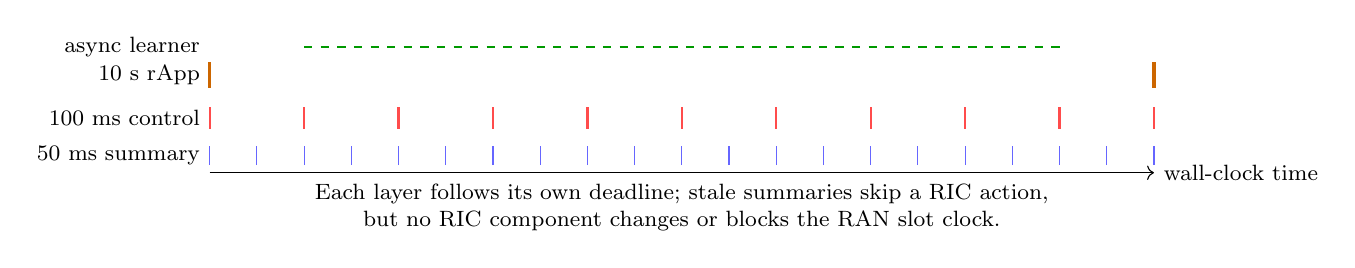
\begin{tikzpicture}[font=\footnotesize,x=0.012cm,y=0.8cm]
\draw[->] (0,0) -- (1000,0) node[right]{wall-clock time};
\foreach \x in {0,50,...,1000} \draw[blue!60] (\x,0.12)--(\x,0.42);
\node[left] at (0,0.28) {50 ms summary};
\foreach \x in {0,100,...,1000} \draw[red!70,thick] (\x,0.7)--(\x,1.05);
\node[left] at (0,0.87) {100 ms control};
\draw[orange!80!black,very thick] (0,1.35)--(0,1.75);
\draw[orange!80!black,very thick] (1000,1.35)--(1000,1.75);
\node[left] at (0,1.55) {10 s rApp};
\draw[green!60!black,thick,dashed] (100,2.0)--(900,2.0);
\node[left] at (0,2.0) {async learner};
\node[align=center] at (500,-0.55) {Each layer follows its own deadline; stale summaries skip a RIC action,\\but no RIC component changes or blocks the RAN slot clock.};
\end{tikzpicture}

  \caption{Independent clocks and data flow. RAN slot processing never waits for monitoring, LLM inference, near-RT control, or asynchronous learning.}
  \label{fig:timing}
\end{figure*}

\subsection{Guided fusion}
\label{subsec:ctl-fusion}
In \texttt{llm\_guided\_ddpg} the LLM target and the learned candidate are fused on integer PRB counts, inside the intersected bounds, rather than in normalized action space:
\begin{equation}
b_A=\mathrm{clip}\!\left(\operatorname{round}\!\left((1-w)\,b_A^{\mathrm{LLM}}+w\,b_A^{\mathrm{DDPG}}\right)+e,\;b_A^{\min},\,b_A^{\max}\right),
\label{eq:ctl-fusion}
\end{equation}
where $b_A^{\mathrm{LLM}}$ is the projected A1 target clipped to the feasible interval, $b_A^{\mathrm{DDPG}}$ is the Actor's projected budget, and $e\sim\mathcal{U}\{-2,\dots,2\}$ PRBs is a teacher-centred jitter applied only while exploring and only before $512$ valid transitions have been collected. Its purpose is to give the critic real responses around the teacher during warm-up while keeping the LLM guardrail; the commanded action, not the Actor output, is what enters replay. The learner reconstructs the continuous analogue of~\eqref{eq:ctl-fusion} as
\begin{equation}
\Pi(u;\ell,h,\tau,w)=\mathrm{clip}\!\left((1-w)\tau+w\left(\ell+u(h-\ell)\right),\,\ell,\,h\right),
\label{eq:ctl-proj}
\end{equation}
with $\ell=b_A^{\min}/N_{\mathrm{PRB}}$, $h=b_A^{\max}/N_{\mathrm{PRB}}$, and teacher $\tau=b_A^{\mathrm{LLM}}/N_{\mathrm{PRB}}$. All of $\ell$, $h$, $\tau$, $w$, and the teacher mask are persisted per transition in \texttt{ddpg\_replay\_transitions.context\_json} and \texttt{next\_context\_json}, so the learner reproduces exactly the bounds and teacher the controller saw.

The execution weight $w$ is the agent's \texttt{guided\_weight}. It starts at $0$, is explicitly reset to $0$ (together with the satisfaction history and the violation counter) after the calibration replay prefill, and is held at $0$ until $512$ valid transitions have accumulated. Thereafter \texttt{update\_guided\_safety()}---called once per completed transition with the \emph{intent}-satisfaction flag, not the SLA flag---raises it by $0.01$ at most once per ten safety updates, and only when the trailing $30$-transition history is full and at least $95\%$ satisfied. The weight is capped at \texttt{max\_ddpg\_weight}${}=0.4$, so the learned policy can never contribute more than $40\%$ of the commanded budget. On five consecutive intent violations the weight is decremented by $0.1$ and action selection forces $w=0$, reverting to the pure LLM action until satisfaction recovers. Because \texttt{update\_guided\_safety()} is invoked outside the training guard, the fusion weight and the fallback counters keep evolving during the frozen evaluation phases; only the Actor, replay ingestion, and the normalization statistics are frozen there.

Guidance also enters the loss. For guided transitions the Actor loss adds a behaviour-cloning term against the projected rApp target,
\begin{equation}
\mathcal{L}_{\mathrm{BC}}=\frac{\sum_i m_i\left(a_i^{\mathrm{proj}}-\tau_i\right)^2}{\max\!\left(\sum_i m_i,\,1\right)},\qquad a_i^{\mathrm{proj}}=\ell_i+u_i(h_i-\ell_i),
\label{eq:ctl-bc}
\end{equation}
compared in projected PRB-fraction space rather than on the raw sigmoid output. The teacher mask $m_i$ is $1$ for every non-calibration guided transition and $0$ for \texttt{ddpg\_only} and for the fixed-ratio calibration sweep. Its weight is $1.0$ for the first $500$ Actor updates and then decays linearly over $1000$ Actor updates to a floor of $0.1$, reaching that floor at Actor update $1500$. Because the guided learner performed $15{,}103$ Actor updates in the pilot, behaviour cloning operated at the $0.1$ floor for roughly $90\%$ of training.

\paragraph*{Relation to the magazine paper's three-phase schedule}
The magazine formulation of \systemname~\cite{bao2026llmhric} trains the guided agent in three discrete phases: guided exploration under the LLM teacher, policy blending with a decaying guidance weight, and self-directed operation. This deployment realizes the same progression, but as a single continuous, safety-gated schedule rather than as scheduled phase boundaries, and with the weight moving in the opposite direction. Concretely: the warm-up before $512$ valid transitions is the analogue of Phase~1---$w=0$, so the commanded action is the teacher plus a $\pm2$~PRB jitter, and the behaviour-cloning weight is at its maximum of $1.0$. The subsequent ramp is the analogue of Phase~2, except that the \emph{teacher} share $1-w$ decays instead of a guidance weight, and it decays only while measured intent satisfaction stays above $95\%$; the behaviour-cloning weight decays on its own actor-step schedule at the same time. Phase~3 is not reached in this deployment: $w$ is capped at $0.4$, so the LLM target always retains at least a $60\%$ share of the commanded budget, and a run of five intent violations returns control to the teacher entirely. The design choice is deliberate---in a live RAN the teacher is retained as a permanent safety envelope rather than as a curriculum that is eventually discarded---but it means the guided arm here is a bounded-authority controller, not the fully self-directed agent of the magazine paper's final phase. Consistently, the pilot's guided arm shows a $90.66\%$ acknowledged-action boundary rate during training, reflecting a commanded action that sits at an endpoint of a narrow calibrated interval most of the time.

\subsection{Asynchronous actor--critic learning}
\label{subsec:ctl-learner}
\paragraph*{Process split}
Inference and learning run in separate OS processes so that no gradient step can extend a control tick; Fig.~\ref{fig:async} summarizes the resulting hand-off, from replay ingestion through candidate scoring to the validated publication of a serving Actor. The campaign driver writes \texttt{effective\_config.json} into the run directory and spawns \texttt{python -m llm\_hric.ddpg\_async\_learner} with \texttt{--config}, \texttt{--run-id}, \texttt{--arm}, \texttt{--checkpoint}, \texttt{--snapshot-dir}, and \texttt{--seed}; the learner is stopped with \texttt{SIGTERM}, a $20$~s grace period, and \texttt{SIGKILL}. The controller is given one PyTorch thread and the learner two. A health check raises on the next controller tick if the learner has exited, so a dead learner fails the run rather than silently freezing the policy. In asynchronous mode the controller's own training branch is unreachable: it neither calls \texttt{train\_step()} nor updates normalization statistics nor writes checkpoints.

\paragraph*{Replay hand-off}
The two processes communicate through SQLite and one atomic file. Each completed transition is appended by \texttt{insert\_replay\_transition()} to \texttt{ddpg\_replay\_transitions}, carrying the raw state and successor state, the commanded action, the raw reward, the terminal flag, the training context and its successor, the policy version, the acknowledgement timestamp, the effect coverage, the validity flag, and the provenance record. Two indices, on \texttt{(run\_id, transition\_id)} and \texttt{(run\_id, transition\_valid, transition\_id)}, support the learner's cursor scan. Calibration-phase transitions are excluded from the controller's insert path and are instead written in bulk by the calibration prefill, which is how the buffer crosses its minimum threshold quickly. The learner polls every \texttt{learner\_poll\_ms}${}=100$~ms with a monotonic \texttt{transition\_id} cursor, reading at most \texttt{ingest\_batch\_size}${}=2048$ rows per poll; it advances the cursor over every row but admits only rows with \texttt{transition\_valid}${}=1$. Each admitted row increments a pending-update counter by one, and each poll performs $\min(32,\,\text{pending})$ gradient steps, so the update-to-data ratio is exactly one. Training is gated on \texttt{min\_replay\_transitions}${}=1000$ buffered rows; a second, lower gate inside the agent requires $128$ rows before any critic update and $512$ before any Actor update. Because publishing and training are disabled during the two frozen evaluation phases, the learner ends a run with a backlog: $15{,}519$ and $16{,}051$ untrained transitions in the guided and unguided pilot runs, against $30{,}207$ and $30{,}266$ completed updates and $45{,}726$ and $46{,}317$ valid replay rows.

\paragraph*{Algorithm}
Although the modules retain the DDPG name for continuity with the magazine paper, the learner implements a TD3-style deterministic actor--critic~\cite{fujimoto2018td3}: twin critics with a clipped double-Q target, target policy smoothing, and delayed Actor updates. The magazine deployment used plain DDPG for power allocation~\cite{bao2026llmhric}, and the code still carries that configuration as its fallback defaults---\texttt{target\_policy\_noise} $0.0$, \texttt{actor\_update\_interval} $1$, \texttt{actor\_saturation\_penalty\_weight} $0.0$, and $\gamma=0.995$. The v5 campaign configuration overrides all four ($0.1$, $2$, $0.01$, and $0.95$), and these overrides were introduced specifically to make the slicing agent converge. We attribute the need for them to the discontinuity of~\eqref{eq:ctl-reward} at the protected floor, across which a single bootstrapping critic over-estimates $Q$ and drives a bounded sigmoid action towards a rail; the clipped double-Q target, the target-action smoothing, and the saturation penalty of~\eqref{eq:ctl-actor} each counteract one part of that failure mode. Both networks are $2\times128$ ReLU MLPs with no shared trunk and no normalization layers. The Actor maps the $24$-D normalized state to a scalar through a \emph{sigmoid} output rather than a $\tanh$, because the action is a normalized PRB fraction in $[0,1]$; each critic concatenates state and action into a $25$-D input.

Per update, a batch of $128$ is drawn, rewards are rescaled as $\tilde r=\mathrm{clip}(r/\sigma_G,-10,10)$ with $\sigma_G$ the running standard deviation of the discounted return ($\gamma=0.95$), and the target is
\begin{align}
u'&=\mathrm{clip}\!\left(\pi_{\phi'}(s')+\mathrm{clip}(\epsilon,-0.25,0.25),\,0,\,1\right),\nonumber\\
a'&=\Pi(u';\ell',h',\tau',w'),\nonumber\\
y&=\tilde r+\gamma(1-d)\min_{i\in\{1,2\}}Q_{\theta_i'}(s',a'),
\label{eq:ctl-target}
\end{align}
with $\epsilon\sim\mathcal{N}(0,0.1^2)$,
$\Pi$ from~\eqref{eq:ctl-proj}, and $d$ the terminal flag. The critic loss is $\mathrm{MSE}(Q_{\theta_1}(s,a),y)+\mathrm{MSE}(Q_{\theta_2}(s,a),y)$, where $a$ is the action actually commanded on the RAN; a single Adam optimizer updates both critics. Every second step, and only once the buffer holds $512$ rows, the Actor is updated with
\begin{equation}
\mathcal{L}_{\pi}=-\mathbb{E}\!\left[Q_{\theta_1}(s,\Pi(u))\right]+\beta_t\,\mathcal{L}_{\mathrm{BC}}+\lambda_{\mathrm{sat}}\,\mathbb{E}\!\left[\left(\max(0,|z|-z_{\max})\right)^2\right],
\label{eq:ctl-actor}
\end{equation}
where $z$ are the pre-activation logits, $z_{\max}=2.944=\mathrm{logit}(0.95)$, and $\lambda_{\mathrm{sat}}=0.01$. The last term is a logit-space saturation penalty: it costs nothing while the Actor operates inside the responsive region of the sigmoid and grows quadratically once it pushes towards either rail, which prevents the gradient-starved boundary collapse that a bounded action with a discontinuous reward otherwise invites. $\beta_t$ is the behaviour-cloning weight of Section~\ref{subsec:ctl-fusion} and is identically zero for \texttt{ddpg\_only}. Gradients are clipped to norm $1.0$ separately for the joint critic parameters and the Actor. The target Actor is soft-updated only inside the delayed branch; both target critics are soft-updated every step with $\tau=0.005$. Minibatches are not drawn uniformly: \texttt{ReplayBuffer.\_balanced\_rows()} bins transitions by the commanded action into ten equal bins and round-robins over shuffled non-empty bins, which keeps the critic's action coverage broad. Per-update diagnostics (critic loss, TD error, predicted and target $Q$, Actor and behaviour-cloning losses, replay size, backlog) are persisted to \texttt{ddpg\_learner\_updates}. Table~\ref{tab:ctl-hyper} lists every hyperparameter with its configuration key. One caveat applies to reading that table against \texttt{config.yaml}: the exploration-noise decay horizon is not the only key the experiment runner rewrites at launch. Before any run starts, the runner also overrides the DDPG control period \texttt{period\_ms.ddpg} (from the spec key \texttt{control\_period\_ms}), the rApp period \texttt{period\_ms.llm} (\texttt{rapp\_period\_ms}), the monitor summary period \texttt{monitor.summary\_period\_ms} (\texttt{monitor\_summary\_period\_ms}), the operational bounds \texttt{control.min\_prb} and \texttt{control.max\_prb} (\texttt{operational\_min\_prb}, \texttt{operational\_max\_prb}), \texttt{ddpg.cell\_prbs} (\texttt{cell\_prbs}), and \texttt{ddpg.model\_version} (\texttt{ddpg\_model\_version}), each falling back to the file value when the spec omits the key. For the v5 spec the overridden values coincide with the file values, so the table is correct as printed, but \texttt{config.yaml} alone is not the record of what a run used: the runner serializes the fully merged configuration to \texttt{<run>/effective\_config.json} and passes that file to the learner, and that file is the authoritative record of the values actually in force.

\begin{table*}[t]
\centering
\footnotesize
\caption{Learner and controller hyperparameters with their \texttt{config.yaml} keys. Values are those used by the v5 campaign.}
\label{tab:ctl-hyper}
\begin{tabular}{llll}
\toprule
Config key & Value & Config key & Value\\
\midrule
\multicolumn{4}{l}{\emph{Networks and optimization} (\texttt{ddpg})}\\
\texttt{hidden\_width} & 128 & \texttt{batch\_size} & 128\\
\texttt{action\_dim} / \texttt{max\_action} & 1 / 1.0 & \texttt{replay\_size} & 100000\\
\texttt{actor\_lr} & $1\times10^{-4}$ & \texttt{gamma} & 0.95\\
\texttt{critic\_lr} (both critics) & $5\times10^{-4}$ & \texttt{tau} & 0.005\\
\texttt{gradient\_clip\_norm} & 1.0 & \texttt{action\_bins} & 10\\
\texttt{actor\_update\_interval} & 2 & \texttt{critic\_learning\_starts} & 128\\
\texttt{target\_policy\_noise} & 0.1 & \texttt{learning\_starts} & 512\\
\texttt{target\_policy\_noise\_clip} & 0.25 & \texttt{cell\_prbs} & 106\\
\texttt{actor\_saturation\_logit\_limit} & 2.944 & \texttt{actor\_saturation\_penalty\_weight} & 0.01\\
\midrule
\multicolumn{4}{l}{\emph{Exploration, normalization, transitions} (\texttt{ddpg})}\\
\texttt{exploration\_noise\_start} & 0.2 & \texttt{exploration\_noise\_end} & 0.02\\
\texttt{exploration\_noise\_decay\_steps} & 14400 (spec-derived) & \texttt{normalization\_freeze\_transitions} & 1000\\
\texttt{state\_normalization} & $\epsilon\,10^{-8}$, clip 5.0, min std 0.05 & \texttt{reward\_scaling} & $\gamma$ 0.95, clip 10.0\\
\texttt{max\_state\_age\_ms} & 1000 & \texttt{transition\_observation\_ms} & 100\\
\texttt{min\_effect\_coverage} & 0.8 & \texttt{checkpoint\_interval\_transitions} & 250\\
\midrule
\multicolumn{4}{l}{\emph{Guidance and safety} (\texttt{ddpg})}\\
\texttt{max\_ddpg\_weight} & 0.4 & \texttt{guided\_weight\_update\_interval} & 10\\
\texttt{sla\_window} & 30 & \texttt{sla\_fallback\_windows} & 5\\
\texttt{bc\_full\_weight\_actor\_steps} & 500 & \texttt{bc\_decay\_actor\_steps} & 1000\\
\texttt{min\_bc\_weight} & 0.1 & & \\
\midrule
\multicolumn{4}{l}{\emph{Asynchronous learning} (\texttt{ddpg.async\_training})}\\
\texttt{learner\_poll\_ms} & 100 & \texttt{ingest\_batch\_size} & 2048\\
\texttt{max\_catchup\_updates} & 32 & \texttt{min\_replay\_transitions} & 1000\\
\texttt{publish\_every\_actor\_updates} & 50 & \texttt{publish\_min\_interval\_s} & 5\\
\texttt{promotion\_holdout\_size} & 1024 & \texttt{snapshot\_poll\_ms} & 500\\
\texttt{max\_promotion\_saturation} & 0.4 & \texttt{max\_promotion\_q\_drop} & 0.02\\
\texttt{max\_promotion\_action\_shift} & 0.2 & \texttt{force\_promotion\_after\_rejections} & 6\\
\texttt{checkpoint\_every\_updates} & 250 & \texttt{require\_initial\_snapshot} & true\\
\texttt{initial\_snapshot\_timeout\_s} & 120 & \texttt{controller\_torch\_num\_threads} & 1\\
\bottomrule
\end{tabular}
\end{table*}

\paragraph*{Candidate promotion}
The learner does not push weights to the controller directly. A candidate is proposed only when at least $50$ Actor updates and $5$~s have elapsed since the last proposal. The candidate is the \emph{target} Actor, and it is scored against the learner's local copy of the currently serving Actor on the most recent $\min(1024,|\mathcal{B}|)$ replay rows, replaying each row's recorded $\ell,h,\tau,w$. Six gates are evaluated in order and each carries a fixed rejection string: (i) all target-Actor parameters and all candidate outputs must be finite; (ii) the saturation rate, the fraction of candidate outputs at or beyond $0.05$ and $0.95$, must not exceed $0.40$; (iii) the mean $Q$ of the candidate's executed action, computed with critic~1 only, must not fall more than $0.02$ below the serving Actor's; (iv) the mean absolute shift of the executed action versus the serving Actor must not exceed $0.20$; (v) the raw outputs must satisfy $0\leq u_{\min}\leq u_{\max}\leq1$; and (vi) the projected action must lie inside $[\ell-10^{-6},h+10^{-6}]\cap[0,1]$ for \emph{every} holdout row. Note that this promotion saturation threshold ($0.05/0.95$, applied to the target Actor on the holdout) is a different quantity from the Actor saturation rate reported in the results, which \texttt{analyze\_results.py} defines as the fraction of raw serving-Actor outputs at or beyond $0.02$ and $0.98$; the two must not be equated.

Because a drifting critic can reject every candidate and starve the controller on a stale or near-random serving Actor---the motivation stated in the source---a fallback force-promotes a candidate after \texttt{force\_promotion\_after\_rejections}${}=6$ consecutive rejections. The forced path still requires gates (i), (v), and (vi); only the saturation, $Q$-drop, and action-shift margins are waived. The rejection counter resets on any acceptance, so the serving Actor can be at most five consecutive candidate evaluations stale. Every candidate, accepted or not, is recorded in \texttt{ddpg\_actor\_versions} with its reason string and full metrics blob, and the version counter increments on every candidate, so version numbers index candidates rather than served snapshots. In the pilot the guided run accepted $62$ of $257$ candidates and the unguided run accepted all $257$; the per-candidate use of the forced path is recorded in the artifact's \texttt{ddpg\_actor\_versions.reason} and \texttt{metrics\_json.forced} fields and is provably zero for the unguided run, which had no rejections.

\paragraph*{Snapshot transport and swap}
An accepted candidate is serialized to \texttt{actor-v\{version\}.pt} via a temporary file and \texttt{os.replace}, its SHA-256 digest is computed by streaming the file, and a manifest \texttt{serving\_actor.json} is written the same way, so the payload always lands before the manifest that references it. The payload carries the target Actor weights, the state normalization statistics, the model and state-feature versions, the state and action dimensions, and a configuration fingerprint---itself a SHA-256 over the slice catalog, feature and model versions, hidden width, action dimension, and cell PRB count. A daemon watcher thread in the controller polls the manifest every $500$~ms, requires a strictly newer version and a matching run identifier, recomputes and compares the digest, loads the payload, and requires the fingerprint to match before staging a deep-copied standby Actor and standby statistics; any torn, foreign, or mismatched snapshot is silently ignored. Only the newest validated snapshot is retained, so intermediates may be skipped. The swap itself is the first thing a controller tick does after schedule bookkeeping and the health check, before state is fetched, and is pure pointer assignment. It was measured at a worst case of $0.662$~ms (guided) and $0.538$~ms (unguided) in the pilot. Before training starts, \texttt{require\_initial\_snapshot} forces the controller to block until a validated Actor and its statistics have been swapped in, with a $120$~s deadline; before each evaluation phase the watcher performs one last swap and is then frozen, which the data confirms with exactly one serving version observed in each evaluation phase for all three arms. Two caveats apply when quoting swap counts: the watcher retains only the newest pending snapshot, and the swap-latency variable is local to a \texttt{run\_controller()} call and is discarded at each block boundary. The number of distinct serving versions actually observed in \texttt{ddpg\_actions} ($61$ guided, $244$ unguided) is therefore the correct measure, not the recorded swap-latency count ($50$ and $204$).

\begin{figure}[t]
  \centering
  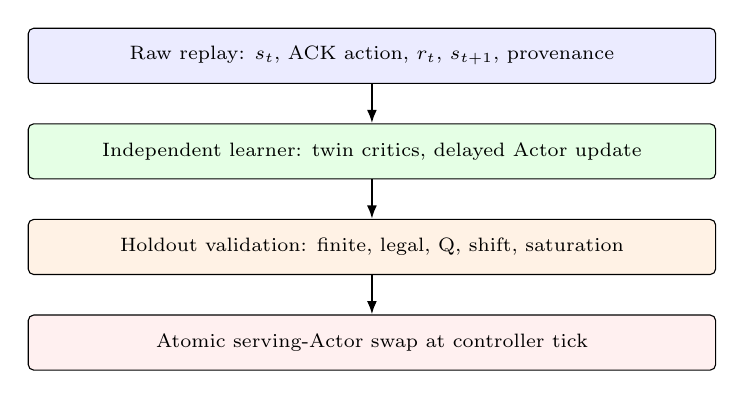
\begin{tikzpicture}[font=\scriptsize,node distance=5mm,
 box/.style={draw,rounded corners=2pt,align=center,minimum width=.72\columnwidth,minimum height=7mm},
 arrow/.style={-{Latex[length=1.7mm]},thick}]
\node[box,fill=blue!8] (replay) {Raw replay: $s_t$, ACK action, $r_t$, $s_{t+1}$, provenance};
\node[box,fill=green!10,below=of replay] (learn) {Independent learner: twin critics, delayed Actor update};
\node[box,fill=orange!10,below=of learn] (validate) {Holdout validation: finite, legal, Q, shift, saturation};
\node[box,fill=red!6,below=of validate] (serve) {Atomic serving-Actor swap at controller tick};
\draw[arrow] (replay)--(learn);
\draw[arrow] (learn)--(validate);
\draw[arrow] (validate)--(serve);
\end{tikzpicture}

  \caption{Asynchronous learner and validated serving-Actor publication.}
  \label{fig:async}
\end{figure}

\subsection{Trained-agent reuse}
\label{subsec:ctl-reuse}
Every learning run archives its agent as \texttt{ddpg.pt} in the run directory. The checkpoint holds the Actor, both critics, all three target networks, both Adam optimizer states, the state normalization and reward scaler states, the replay buffer, the learner counters (\texttt{train\_steps}, \texttt{actor\_update\_steps}, \texttt{valid\_transitions}, \texttt{last\_replay\_transition\_id}, \texttt{actor\_version}), the guided-safety state (\texttt{guided\_weight}, \texttt{sla\_history}, \texttt{consecutive\_violations}, \texttt{safety\_update\_steps}), the seed, and both the Python and PyTorch RNG states. Loading hard-fails on any mismatch of \texttt{model\_version}${}=4$, \texttt{state\_feature\_version}${}=3$, \texttt{replay\_schema\_version}${}=3$, state dimension, or action dimension, so an incompatible agent can never be silently reused. The learner writes a slim checkpoint (replay omitted, because serializing it dominates file size at hundreds of megabytes) every $250$ training steps and one full checkpoint on shutdown.

Two re-evaluation paths are provided, and neither modifies the source checkpoint. The first is offline and needs no RAN stack:
\begin{quote}\footnotesize\ttfamily
python -m llm\_hric.experiments.eval\_checkpoint\\
\ \ --checkpoint <run>/ddpg.pt\\
\ \ --db <run>/llm\_hric.sqlite3\\
\ \ --phase training --limit 20000\\
\ \ --plot <run>/policy\_response.png
\end{quote}
It reads the most recent valid rows of \texttt{ddpg\_replay\_transitions}, runs the deterministic Actor without exploration noise, applies~\eqref{eq:ctl-proj} with each row's recorded $\ell,h,\tau,w$, and reports the loaded counters, the mean and $95$th-percentile disagreement in PRBs between the deterministic policy and the actions that were executed live, the Actor saturation rate, and---split by intent direction using the Slice-A priority one-hot at state index $9$---the allocation mean, standard deviation and range, the mean critic $Q$, and the mean recorded reward. The optional plot writes a per-intent allocation histogram with reference lines at $45\%$ and $55\%$.

The second re-runs the full protocol against a frozen policy on the live testbed, taking roughly twelve minutes per run:
\begin{quote}\footnotesize\ttfamily
python -u -m llm\_hric.experiments.experiment\_runner\\
\ \ --spec llm\_hric/experiments/five\_ue\_traffic\_scenarios\_v5.json\\
\ \ --results /tmp/llm\_hric/experiments/five-ue-traffic-v5-eval\\
\ \ --manage-stack --seed 1 --fail-fast\\
\ \ --scenario balanced --arm ddpg\_only\\
\ \ --eval-checkpoint <run>/ddpg.pt
\end{quote}
This mode requires \texttt{--arm} and an existing file, copies the checkpoint into a fresh run directory, disables asynchronous training so that no learner is spawned and the controller takes the synchronous path with training and exploration off, and raises if the checkpoint fails to load. It skips calibration-guidance collection, the calibration replay prefill, and the entire training phase, validating only the calibration and the two evaluation phases. The run identifier carries an \texttt{-evalck} tag, the manifest records \texttt{"mode": "eval\_checkpoint"} together with the source path, and such runs are excluded from resume bookkeeping so that they can never mask a real training run. Results are scored with the same \texttt{analyze\_results.py} pipeline pointed at the dedicated results directory. Both paths, the checkpoint format, and the campaign specification are part of the released artifact at \codeurlprinted.

\begin{table*}[t]
\centering
\caption{Application interfaces, inputs, outputs, and clocks.}
\label{tab:apps}
\begin{tabular}{lllll}
\toprule
Component & Input & Output & Interface/store & Nominal period\\
\midrule
SM monitor & MAC/RLC/PDCP/GTP indications & raw counters, slice summaries & E42, SQLite & 10~ms / 50~ms\\
KPM collector & E2SM-KPM indications & audit measurements & E2, SQLite & configured subscription\\
Gemma rApp & intent, three 10~s windows & target, bounds, confidence & A1-like HTTP/SQLite & 10~s\\
near-RT controller & 24-D state, active policy & complementary PRB budgets & Unix socket, E2SM-RC & 100~ms\\
asynchronous learner & valid replay rows & validated Actor snapshot & SQLite table, atomic file & 100~ms poll\\
serving-Actor watcher & snapshot manifest & staged Actor + statistics & sha256-verified file & 500~ms poll\\
OAI scheduler & active dedicated ratios & per-slot new-data grants & gNB internal & slot-level\\
\bottomrule
\end{tabular}
\end{table*}

\section{Experimental Methodology}
\label{sec:methodology}
\label{sec:methodology-anchor}
The campaign is defined by a single JSON specification,
\texttt{experiments/five\_ue\_traffic\_scenarios\_v5.json}
(\texttt{protocol\_version}~8, SHA-256 \texttt{7f1d5c03\ldots fea025d}), and executed by
\texttt{experiments/experiment\_runner.py}. The specification fixes three traffic scenarios,
three arms, five seeds, the 106-PRB cell, the 100~ms control period, the 50~ms monitor
summary period, the 10~s rApp period, every phase duration, and every validity threshold.
Nothing in the protocol below is a per-run operator decision. At launch the runner copies the
specification over the static controller configuration --- the DDPG control period and the
rApp period in \texttt{period\_ms}, \texttt{monitor.summary\_period\_ms},
\texttt{operational\_min\_prb}/\texttt{operational\_max\_prb} into
\texttt{control.min\_prb}/\texttt{control.max\_prb}, the cell PRB count
\texttt{ddpg.cell\_prbs}, \texttt{ddpg.model\_version}, the channel-profile enable flag, and
the spec-derived \texttt{exploration\_noise\_decay\_steps} --- and writes the merged
configuration to \texttt{<run>/effective\_config.json}, which is the authoritative record of
what a run actually executed with.

\subsection{Compared control arms and their ablation}
Three arms are compared. Their code identifiers are \texttt{llm\_only}, \texttt{ddpg\_only},
and \texttt{llm\_guided\_ddpg}; in the text we call them LLM-only, DDPG-only (TD3-style), and
LLM-guided. The generated tables emitted by \texttt{scripts/build\_results.py} label the same
three arms ``LLM only'', ``TD3 only'', and ``LLM-guided TD3''.

\begin{itemize}
  \item \texttt{llm\_only} executes the rApp target. The published ratios are projected into
  the intersection of the A1 guidance bounds and the operational envelope, converted to an
  integer Slice-A budget, and commanded every 100~ms. The target itself is refreshed only
  every 10~s, so this arm holds one action between rApp updates. No actor--critic is used and
  no learner process is started.
  \item \texttt{ddpg\_only} executes the learned actor. It is an ablation of guidance, not of
  the task: it keeps the identical 24-dimensional state layout, the identical SLA-gated
  reward with the same weights, the identical intent semantics (priority slice, protected
  slice, floor $F$, and minimum priority ratio), and the identical calibration profile of its
  seed. What is removed is the LLM itself. In \texttt{state\_vector} the guidance flag is
  false, so both projected-target features are zeroed; the arm is bounded only by the
  operational envelope and never intersects the A1 \texttt{policy\_constraints}; the
  behavioral-cloning teacher term is disabled (\texttt{teacher\_mask}${}=0$, so the actor loss
  reduces to the deterministic policy-gradient term plus the saturation penalty); and the
  intent-triggered fallback to the LLM action does not exist.
  \item \texttt{llm\_guided\_ddpg} commands a convex blend
  $b_A=(1-w)\,b_A^{\mathrm{LLM}}+w\,b_A^{\mathrm{RL}}$ clipped to the active feasible
  interval. The learned weight $w$ starts at $0$, rises by $0.01$ every ten safety updates
  while the last 30 \emph{intent} outcomes are at least 95\% satisfied, is capped at
  \texttt{max\_ddpg\_weight}${}=0.4$, and is reduced by $0.1$ (and forced to $0$ for command
  purposes) after five consecutive \emph{intent} violations. The trigger is the
  intent-satisfaction flag and not SLA satisfaction: \texttt{update\_guided\_safety} is
  invoked with the per-transition intent-satisfied component, even though the fixed-length
  window it appends to is misleadingly named \texttt{sla\_history}. The distinction is
  material rather than cosmetic, because intent satisfaction is the strictly stronger of the
  two conditions defined below and the two diverge widely in the pilot
  (Section~\ref{sec:results}). During critic warm-up the commanded budget is additionally
  dithered by $\pm2$ PRBs around the teacher. The commanded action, not the raw actor output,
  is what enters replay.
\end{itemize}

Table~\ref{tab:proto-arms} summarizes the ablation. Because the objective and the state
layout are shared, a difference between \texttt{ddpg\_only} and \texttt{llm\_guided\_ddpg}
is \emph{not} attributable to a different task definition. It is not thereby attributable to
guidance alone: Section~\ref{sec:limitations} records a residual confound in episode
termination---the guided arm's terminal flag fires on every 10~s A1 policy version bump,
whereas the unguided arm's fires only at an intent switch, so the two arms bootstrap over
episodes of different length---and a single seed cannot separate policy effects from seed
effects.

\begin{table}[t]
\centering
\footnotesize
\setlength{\tabcolsep}{4pt}
\caption{Ablation across the three arms. ``Intent semantics'' covers the priority/protected
identities, the calibrated floor $F$, and the 55\% minimum priority ratio. The
intent-violation row is the fallback to the LLM action after five consecutive intent
violations; it is driven by intent satisfaction, not by SLA satisfaction.}
\label{tab:proto-arms}
\begin{tabular}{lccc}
\toprule
Component & LLM-only & DDPG-only & LLM-guided\\
\midrule
Intent semantics in reward      & yes & yes & yes\\
24-D state layout               & yes & yes & yes\\
Projected A1 target in state    & yes & zeroed & yes\\
A1 guidance bounds applied      & yes & no & yes\\
Operational 10--90\% envelope   & yes & yes & yes\\
Learned actor--critic           & no  & yes & yes\\
Teacher (BC) loss term          & --- & no  & yes\\
Intent-violation LLM fallback   & --- & no  & yes\\
Asynchronous learner started    & no  & yes & yes\\
\bottomrule
\end{tabular}
\end{table}

\subsection{Run protocol and step budget}
A run executes the phases of Table~\ref{tab:proto-phases}. Phase durations are converted to
control steps by \texttt{\_phase\_steps} as
$\operatorname{round}(\text{seconds}\times1000/\text{period})$; with the 100~ms period
this yields 1{,}000 calibration, 36{,}000 training, and $1{,}800+1{,}800$ evaluation steps,
i.e.\ 40{,}600 counted transitions per run. \texttt{\_validate\_run} compares the per-phase
transition counts in \texttt{experiment\_steps} against these exact values and aborts the run
on any mismatch, so a partially executed phase can never enter the results.

\begin{table}[t]
\centering
\footnotesize
\caption{Per-run phase budget at the 100~ms control period.}
\label{tab:proto-phases}
\begin{tabular}{lrrll}
\toprule
Phase & Dur.\ (s) & Steps & Learning & Active intent\\
\midrule
\texttt{settle}        & 30   & ---     & ---      & bootstrap\\
\texttt{calibration}   & 100  & 1{,}000 & replayed & bootstrap\\
\texttt{intent\_switch}& var. & var.    & training only & regenerating\\
\texttt{training}      & 3600 & 36{,}000& on       & alternating\\
\texttt{intent1\_eval} & 180  & 1{,}800 & frozen   & Intent~1\\
\texttt{intent2\_eval} & 180  & 1{,}800 & frozen   & Intent~2\\
\midrule
counted total          & 4060 & 40{,}600 & & \\
\bottomrule
\end{tabular}
\end{table}

Before settling, the runner installs a bootstrap intent (Intent~1 with a 10~Mbps placeholder
floor and no policy constraints), waits for the first rApp guidance, verifies UE reachability,
and starts the iperf3 servers and clients. It then holds that state for 30~s while the runtime
watchdog polls every subsystem, so the calibration sweep already observes a loaded cell.

During training the active intent alternates every 600 control steps, i.e.\ every 60~s of
\emph{counted} control, giving 60 blocks and therefore 30 blocks (18{,}000 steps) per
direction. Between two blocks the controller does not pause: the runner spawns a worker that
rewrites the intent and waits for the A1 policy and rApp guidance to be regenerated, while
\texttt{run\_controller} keeps issuing actions under the phase label \texttt{intent\_switch}
with \texttt{max\_steps=None}. Those transitions are logged, and during training they are also
inserted into the replay, but they are excluded from the validated per-phase budget. The
wall-clock spacing between intent switches therefore exceeds 60~s. Empirically the surplus is
substantial: the asynchronous replay held 45{,}726 rows for the guided arm and 46{,}317 for
the unguided arm against 1{,}000 prefilled plus 36{,}000 training transitions, i.e.\
approximately $8.7\times10^3$ and $9.3\times10^3$ uncounted switch transitions per run.

Exploration noise is scheduled against the specification rather than the static
configuration: \texttt{exploration\_noise\_decay\_steps} is overridden to
$\operatorname{round}(0.4\times36{,}000)=14{,}400$, so Gaussian action noise decays linearly
from $0.2$ to $0.02$ over the first 40\% of training and leaves a 21{,}600-step low-noise
exploitation tail before evaluation.

Both evaluation phases are frozen. The runner sets the runtime state to
\texttt{train=False, publish=False}, then calls \texttt{freeze()} on the Actor-snapshot
watcher, which pins the serving Actor and sets \texttt{stats\_frozen}, so observation
normalization and reward scaling also stop updating. The freeze is verifiable in the artifact:
every arm reports exactly one distinct serving Actor version in each evaluation phase.

\subsection{Calibration}
Calibration is a fixed open-loop sweep, not a search and not a fourth policy. Slice~A is held
at each of 25\%, 35\%, 50\%, 65\%, and 75\% for 200 control steps (20~s) each, driven through
\texttt{experiment.fixed\_slice\_a\_ratio}, which makes the controller behave as a static
allocator regardless of arm. Three quantities are then derived.

\begin{enumerate}
  \item \emph{Cell capacity.} The runner sums \texttt{dl\_th\_mbps} over slices per
  \texttt{ts\_ms} in \texttt{network\_state} for the whole 100~s sweep and takes the
  linearly interpolated 95th percentile of those per-summary cell totals. The result is stored
  as \texttt{experiment.capacity\_mbps} and is the denominator of the normalized total and
  priority throughput terms in the reward, so every reward value is relative to this per-seed
  capacity estimate.
  \item \emph{Protected-slice floor.} Per-slice throughput samples are bucketed by the sweep
  level nearest to the acknowledged Slice-A ratio. For each intent the runner takes the
  reference allocation (65\% Slice-A for Intent~1, 35\% for Intent~2), computes the
  nearest-rank 10th percentile of the \emph{protected} slice throughput at that allocation,
  and sets $F=0.90\times p_{10}$. The floor is therefore a 10\% margin below an already
  pessimistic observed level, is per seed and per testbed, and is rendered into the
  natural-language intent string with two decimals through the \texttt{\{floor\_mbps\}}
  placeholder. Calibration raises and fails the run if $F\le0$ or if the reference allocation
  is not itself feasible.
  \item \emph{Guidance bounds.} A sweep level is labelled safe post hoc if its protected-slice
  $p_{10}$ meets $F$ and it respects the intent's direction. Writing $\mathcal{S}$ for that
  set, Intent~1 publishes Slice~A in $[55\%,\max\mathcal{S}]$ and Intent~2 publishes Slice~A
  in $[\min\mathcal{S},45\%]$, with complementary bounds for Slice~B. These are exported as
  A1 \texttt{policy\_constraints}.
\end{enumerate}

The 10--90\% envelope is \emph{not} a calibration product. It is the specification constant
pair \texttt{operational\_min\_prb}${}=10$ / \texttt{operational\_max\_prb}${}=90$, copied into
\texttt{control.min\_prb} / \texttt{control.max\_prb} before any run and applied by
\texttt{\_global\_bounds} to every arm. For the 106-PRB cell it gives the integer interval
$b_A\in[11,95]$. Only \texttt{llm\_only} and \texttt{llm\_guided\_ddpg} intersect the
calibration bounds with this envelope; \texttt{ddpg\_only} sees the envelope alone. With the
55\% minimum priority ratio the guided Intent-1 interval starts at
$b_A^{\min}=\max(\lceil 55\cdot106/100\rceil,\,106-\lfloor 45\cdot106/100\rfloor)=59$ and the
guided Intent-2 interval ends at $b_A^{\max}=47$, independently of $\mathcal{S}$.

The calibration profile is written to
\texttt{<scenario>/seed-<N>-calibration-profile.json} and reused by the remaining arms of the
same (scenario, seed) cell when the profile version matches. All three arms of a seed thus
share one capacity estimate, one floor, and one bound set, which is what makes the paired
comparison meaningful. Finally the 1{,}000 calibration transitions are replayed into the
learner buffer of the two learning arms with synthetic guidance that alternates every 100
steps, and the agent's SLA history, violation counter, and guided weight are reset before and
after the prefill so that calibration cannot bias the safety state machine.

\subsection{Traffic generation}
Each UE is served by one persistent iperf3 UDP client started inside the external data-network
container and addressed to the UE PDU IP, and by one iperf3 server bound to that PDU IP inside
the UE network namespace. There is exactly one stream and one port per UE; there is no
separate burst stream. The client duration is the larger of 3600~s and the specification key
\texttt{traffic\_max\_duration\_s}, i.e.\ 86{,}400~s, so that traffic never expires mid-run.

For dynamic scenarios the client is offered that UE's \emph{phase-maximum} rate for the whole
run and the phase pattern is realized in the network rather than at the source. The controller
installs an HTB qdisc on the external data-network egress device (\texttt{root handle 1:},
\texttt{r2q 100}, \texttt{default 999}, root and default classes at \texttt{1000mbit}), one
class \texttt{1:10}$x$ per UE with a \texttt{pfifo limit 100} child and a \texttt{u32} filter
matching the UE PDU address as a \texttt{/32}. Every 5~s the scheduler rewrites all five
classes with a single batched \texttt{tc class change ... htb rate Xmbit ceil Xmbit}. The
balanced scenario has a single phase, so no shaper is installed and the clients simply run at
the constant 30~Mbps per-UE rate; \texttt{traffic\_summary.json} records this as
\texttt{traffic\_backend}${}=$\texttt{iperf3} rather than \texttt{tc\_htb}.

Shaper fidelity is audited per segment. At the end of each UE $\times$ 5~s segment the
controller reads that UE's HTB class byte counter, computes the actual egress rate over the
elapsed interval, and accepts the segment only if it lasted at least $0.8\times5=4$~s and
delivered between 80\% and 125\% of the requested rate. The run-level
\texttt{dynamic\_segment\_success\_rate} divides valid segments by
$\lfloor D/5\rfloor$ (plus one if the remainder is at least 4~s) times five UEs, and the run is
rejected below 0.95. In the balanced pilot the shaper is never installed, so the reported
segment success rate of 100\% is vacuous and must not be read as evidence of shaper fidelity.

Receiver-side goodput is measured from the UE TUN interface \texttt{rx\_bytes} delta over the
measurement window. The reported loss percentage is
$100\,(1-\text{received}/\text{offered})$ where ``offered'' is the scenario's nominal mean
per-UE rate; it is an offered-versus-delivered figure computed at the receiver, not the
iperf3 sender's own datagram-loss report. Traffic phase applications are logged to a
\texttt{traffic\_events} table with planned and applied timestamps, and the trace is hashed so
that different arms can be shown to have seen identical offered load.

\subsection{Validity gates}
Table~\ref{tab:proto-gates} lists every check applied by \texttt{\_validate\_run}. A raising
check marks the run \texttt{failed}; the five-UE coverage check is non-fatal but marks the run
\texttt{degraded}. \texttt{scripts/build\_results.py} discards anything that is not
\texttt{status=complete} and \texttt{data\_quality=primary} before it opens a database, so
neither class can reach a table.

\begin{table*}[t]
\centering
\footnotesize
\caption{Validity gates. ``Spec'' checks read the campaign specification; ``code'' checks are
hardcoded in \texttt{experiment\_runner.py}. Async-only checks apply to \texttt{ddpg\_only}
and \texttt{llm\_guided\_ddpg}.}
\label{tab:proto-gates}
\begin{tabular}{llll}
\toprule
Check & Threshold & Source & Effect\\
\midrule
Per-phase transition count & exactly 1{,}000 / 36{,}000 / 1{,}800 / 1{,}800 & spec durations & fail\\
RC apply success rate & $\geq0.99$ (\texttt{min\_apply\_success\_rate}) & spec & fail\\
Mapped UEs & $\geq1$ under \texttt{allow\_ue\_churn}, else exactly 5 & spec & fail\\
Transitions with effect coverage $\geq0.8$ & $\geq95\%$ & code & fail\\
RC control latency p99 & $<20$~ms & code & fail\\
Controller tick jitter p95 / p99 & $\leq120$ / $\leq150$~ms & spec & fail (async)\\
Fresh-state action interval p95 & $\leq180$~ms & spec & fail (async)\\
Controller stale-skip rate & $\leq0.5$ & spec & fail (async)\\
Controller tick telemetry present & non-empty & code & fail (async)\\
Traffic summary parseable & --- & code & fail\\
Valid iperf UEs & $\geq1$ (\texttt{min\_valid\_traffic\_ues}) & spec & fail\\
Traffic event success rate & $\geq0.99$ & spec & fail\\
Dynamic segment success rate & $\geq0.95$ & spec & fail\\
Dynamic-channel command success / coverage & 100\% & code & fail (if enabled)\\
Five-UE coverage & $\geq0.90$ (\texttt{primary\_five\_ue\_coverage}) & spec & degrade\\
\bottomrule
\end{tabular}
\end{table*}

Two specification keys are computed and archived but never enforced and must not be described
as gates: \texttt{max\_fresh\_action\_interval\_p99\_ms}${}=300$ is recorded in the validation
block without an assertion, and \texttt{max\_summary\_age\_ms}${}=3000$ is never read by the
runner. One gate is also weaker than it appears: the mapped-UE query counts distinct
\texttt{ue\_id} values over the whole database without a run or time filter, so when several
runs share one database it does not isolate the run under test. Five-UE coverage, which is
computed strictly inside the run's own transition window, is the check that actually
constrains per-run UE presence.

Per-transition trainability is decided independently of these run-level gates. A transition
enters the replay only if the control was acknowledged, at least one UE was active, the number
of mapped UEs equals the number of active UEs, no counter reset occurred in the window, all
metric sources were valid, and the action-effect window coverage was at least 0.8.

\subsection{Reported metrics and their definitions}
All phase metrics are computed by \texttt{analyze\_results.\_step\_metrics} over the
transitions of a phase. Two definitions carry most of the interpretation and are used
throughout Section~\ref{sec:results-anchor}:

\begin{itemize}
  \item \emph{SLA satisfaction} is the fraction of transitions whose normalized protected-slice
  deficit is zero, i.e.\ the protected slice met its floor $F$ (or the floor was inapplicable
  because $F\le0$ or the protected slice carried no UE).
  \item \emph{Intent satisfaction} is the fraction of transitions that satisfy the SLA
  \emph{and} command the priority slice at least its minimum ratio of 55\%. It is therefore a
  strictly stronger condition, and the gap between the two is a commanded-allocation property,
  not a throughput shortfall.
\end{itemize}

The remaining reported quantities are: SLA deficit area (the sum of positive normalized
deficits over a phase), protected-slice 5th-percentile throughput, aggregate and per-slice
RLC-derived throughput, UE-level and slice-level Jain fairness, commanded and KPM-measured PRB
share, RLC buffer occupancy, receiver goodput and offered-versus-delivered loss, RC control
latency, controller tick jitter, stale-state skip rate, learner TD error, and Actor
diagnostics. The Actor diagnostics are: saturation rate (fraction of raw actor outputs at or
beyond $0.02$/$0.98$), action-bin coverage (visited tenths of the unit action range, out of
ten), and acknowledged-action boundary rate (fraction of commanded Slice-A budgets within half
a PRB of an edge of that transition's own feasible interval). Early-phase diagnostics use the
first 300 training transitions; ``reward AUC'' is the sum of raw rewards over that window.
Downlink BLER and wideband CQI are recorded but are effectively unpopulated under the
\texttt{static\_awgn} RFSimulator profile used here, and are consequently not interpreted as
measured radio quality.

\ifFullCampaign
The complete campaign uses same-seed paired bootstrap confidence intervals.
\else
The complete campaign will use same-seed paired bootstrap confidence intervals.
\fi
A single-seed pilot cannot estimate run-to-run uncertainty; repeated windows inside one run
are not treated as independent seeds.

\subsection{Reproducibility}
\textbf{Seeding.} Each run calls \texttt{random.seed(seed)} in the runner, and the agent seeds
both Python's RNG and \texttt{torch} with the run seed in the controller process and again in
the learner subprocess, which is launched with \texttt{--seed}. Dynamic-channel traces, when
enabled, are drawn with derived seeds $s$, $s+10^4$, and $s+2\times10^4$ for the training and
two evaluation phases. Arm execution order inside a (seed, scenario) cell is shuffled
deterministically from the string \texttt{"seed:scenario"} so that arm order is not confounded
with time. NumPy, CUDA kernels, and cuDNN determinism flags are not seeded or forced, and the
learner advances on wall-clock rather than in lockstep with the controller; runs are therefore
statistically, not bitwise, reproducible.

\textbf{Isolation.} Every run gets its own result directory containing its checkpoint
(\texttt{ddpg.pt}), Actor-snapshot directory, effective configuration, learner log, archived
component logs, traffic summary and shaper-segment file, manifest, and an end-of-run SQLite
backup of the database. The live database is \emph{not} per run: it is the single shared file
\texttt{/tmp/llm\_hric/llm\_hric.sqlite3}. It is deleted, together with its WAL/SHM files and
the actuator socket, only inside \texttt{restart\_stack}, which the runner invokes only when
started with \texttt{--manage-stack}; that flag also tears down and relaunches the whole
RFSimulator stack (\texttt{UE\_MODE=multi}, \texttt{UE\_COUNT=5}, monitor and guidance
services enabled, standalone DDPG disabled) before every arm/seed and then waits up to 180~s
for preflight. Campaign runs must therefore be launched with \texttt{--manage-stack};
without it, a run appends to whatever database is already present.

\textbf{Resume and failure handling.} \texttt{--resume} scans archived manifests and skips any
(scenario, arm, seed) tuple already recorded as complete or degraded, making the campaign
idempotent across interruptions; frozen-policy re-evaluation manifests are ignored by this
scan, and dynamic-scenario runs produced by the superseded host-side termination path are
deliberately not counted as complete and are retried. \texttt{--fail-fast} aborts after
archiving the first failed run; otherwise failures are accumulated and re-raised at the end so
that one bad cell does not cost the rest of the campaign. Preflight is mandatory and requires
a GPU unless \texttt{--allow-no-gpu} is given.

\textbf{Cost.} Measured from the run manifests, a single run takes 5{,}113--5{,}276~s
(85.2--87.9~min) of wall clock against a 4{,}090~s nominal phase budget. The roughly 27\%
overhead is dominated by the 64 intent switches per run (two after calibration, 60 between
training blocks, and one before each evaluation), each of which waits for a fresh rApp
inference at the 10~s rApp period, plus stack settling and traffic prefill. At the observed
mean of 5{,}210~s per run, the complete $3\times3\times5$ campaign requires approximately
65~hours of continuous testbed time excluding stack restarts.

\textbf{Environment.} Table~\ref{tab:proto-env} lists the testbed. The single 8~GB laptop GPU
hosts both the 4-bit quantized Gemma rApp and the TD3-style networks; the controller is
restricted to one Torch thread and the learner to two so that inference cannot starve the
100~ms control loop. The runner records the GPU model, driver, Python, and Torch/Transformers
versions into every manifest, so a single future run restores this block exactly; the values
below were probed on the testbed host because the pilot manifests were stored under
\texttt{/tmp} and are no longer available.

\begin{table}[t]
\centering
\footnotesize
\caption{Testbed hardware and software.}
\label{tab:proto-env}
\begin{tabular}{ll}
\toprule
Item & Value\\
\midrule
GPU & NVIDIA GeForce RTX 4060 Laptop, 8188~MiB, driver 580.173.02\\
CPU & Intel Core i7-13650HX, 1 socket, 14 cores, 20 threads\\
RAM & 31~GiB\\
OS & Ubuntu 22.04.5 LTS, kernel 6.5.0-18-generic\\
PyTorch & 2.7.0+cu118\\
OAI revision & \texttt{cb0e5012}\\
FlexRIC revision & \texttt{340c36bc}\\
\bottomrule
\end{tabular}
\end{table}

\textbf{Artifact custody.} The primary evidence for every number in
Section~\ref{sec:results-anchor} is the per-run SQLite backup (1.0--1.3~GB per run) plus its
manifest. These files were written under \texttt{/tmp} in the pilot and have since been lost
with the host's temporary directory; the committed \texttt{generated/} CSV and \LaTeX{}
artifacts are what remain. Future campaign runs must therefore use a \texttt{--results}
directory outside \texttt{/tmp}, and the databases must be archived with the paper.

\section{Deployment Results}
\label{sec:results}
\label{sec:results-anchor}
\InputIfFileExists{generated/results_status.tex}{}{}

\subsection{Artifact status and closed-loop reliability}
At the time of writing, \ValidRunCount{} of the \ExpectedRunCount{} planned primary runs are
available. They cover \AvailableScenarioCount{} traffic scenario(s) and
\AvailableSeedCount{} distinct seed(s). Failed and superseded runs are excluded by manifest
status and data quality before any database is opened: the pilot's exclusion list contains
exactly one entry, an earlier \texttt{ddpg\_only} seed-1 attempt that did not reach
\texttt{status=complete}. Two integrity caveats belong with these counts. First, the selector
keys candidate runs on the (scenario, arm, seed) triple and keeps the newest one; it does not
read the manifest \texttt{mode} field, so a frozen-policy re-evaluation run --- which validates
against a reduced phase set and can legitimately be marked complete and primary --- would
supersede the training run of the same cell. Such runs must be written to a separate results
directory until the selector filters on \texttt{mode}. Second, the raw evidence for this pilot
no longer exists. The three per-run SQLite databases ($\approx$1.3~GB each) and the trained
checkpoints were written to a results directory under \texttt{/tmp}; the testbed host was
subsequently rebooted to repair an NVIDIA driver/library version mismatch, and \texttt{/tmp} is
cleared on reboot, so those databases and checkpoints are permanently lost. What survives is
the derived artifact committed under \texttt{generated/}: \texttt{run\_metrics.csv} (213
columns, one row per selected run), \texttt{selected\_runs.csv}, the generated \LaTeX{} tables,
the three figures, and \texttt{artifact\_manifest.json}, which records the specification
SHA-256 and the OAI and FlexRIC revisions. Every number reported below therefore remains
traceable to a committed CSV column, but none of them can be re-derived from raw data and
\texttt{make results} can no longer regenerate the artifact. The campaign runs must archive
their databases on a persistent path rather than under \texttt{/tmp}.

\IfFileExists{generated/control_table.tex}{\begin{table*}[t]
\centering
\caption{Balanced seed-1 control-path and asynchronous learner reliability.}
\label{tab:pilot-control}
\begin{tabular}{lrrrrrr}
\toprule
Arm & Apply success (\%) & RC p99 (ms) & Tick p99 (ms) & Stale skip (\%) & Learner updates & Accepted Actors\\
\midrule
LLM-guided TD3 & 100.00 & 2.80 & 107.02 & 1.19 & 30207 & 62 \\
LLM only & 100.00 & 3.10 & 66.87 & 0.39 & 0 & 0 \\
TD3 only & 100.00 & 2.87 & 93.38 & 1.00 & 30266 & 257 \\
\bottomrule
\end{tabular}
\end{table*}
}{No generated control table is available.}

As Table~\ref{tab:pilot-control} records, all three selected runs reported 100\% five-UE
coverage over their own transition window and received an E2 acknowledgement for every
recorded control (apply success 100\%). The
persistent actuator kept RC control latency in the low-millisecond range, with a p99 of
2.80--3.10~ms against the 20~ms bound. Controller tick jitter p99 was 66.87--107.02~ms against
the 150~ms bound, and the stale-state skip rate was 0.39--1.19\% against the 50\% bound. The
measured fresh-state action interval averaged 101.3--103.6~ms, slightly above the nominal
100~ms clock, because a tick that sees no newer 50~ms summary is skipped rather than
fabricating a transition; its p95 was 166~ms for all three arms, inside the enforced 180~ms
bound, while the p99 of 208--231~ms is recorded but not gated.
\FloatBarrier

\subsection{Intent satisfaction and throughput}
Throughout this section, \emph{SLA satisfaction} is the fraction of control steps in which the
protected slice met its calibrated floor, and \emph{intent satisfaction} is the strictly
stronger condition that the SLA holds \emph{and} the commanded PRB share of the priority slice
is at least the configured minimum of 55\%. Throughput figures are RLC-derived aggregates from
the near-RT state, not iperf receiver goodput.

\ifFullCampaign
\IfFileExists{generated/campaign_table.tex}{\begin{table*}[t]
\centering
\caption{Complete-campaign scenario means. Statistical comparisons use paired seeds rather than these unpaired row means.}
\label{tab:campaign-performance}
\begin{tabular}{llrrrrr}
\toprule
Scenario & Arm & Seeds & I1 satisfaction (\%) & I2 satisfaction (\%) & I1 total TH & I2 total TH\\
\midrule
balanced & LLM-guided TD3 & 1 & 100.00 & 99.94 & 97.35 & 96.44 \\
balanced & LLM only & 1 & 99.94 & 99.39 & 94.58 & 92.14 \\
balanced & TD3 only & 1 & 79.94 & 69.78 & 95.49 & 93.73 \\
\bottomrule
\end{tabular}
\end{table*}
}{No generated campaign table is available.}
\IfFileExists{generated/paired_table.tex}{\begin{table*}[t]
\centering
\caption{Same-seed paired bootstrap comparisons. Positive values favor guided control.}
\label{tab:paired-results}
\begin{tabular}{lllrrl}
\toprule
Scenario & Comparison & Metric & Pairs & Mean difference & 95\% CI\\
\midrule
balanced & Guided $-$ TD3 only & Intent satisfaction & 1 & 0.251 & [0.251, 0.251] \\
balanced & Guided $-$ TD3 only & Total DL TH & 1 & 2.277 & [2.277, 2.277] \\
balanced & Guided $-$ LLM only & Intent satisfaction & 1 & 0.003 & [0.003, 0.003] \\
balanced & Guided $-$ LLM only & Total DL TH & 1 & 3.536 & [3.536, 3.536] \\
\bottomrule
\end{tabular}
\end{table*}
}{}
The complete campaign is analyzed per scenario with same-seed pairing in
Table~\ref{tab:campaign-performance} and Fig.~\ref{fig:pilot-performance}; cross-scenario values are equal-weight macro averages rather than pooled windows.
\else
The available data constitute a balanced-load seed-1 pilot.
\IfFileExists{generated/performance_table.tex}{\begin{table*}[t]
\centering
\caption{Balanced seed-1 pilot. Satisfaction is the fraction of frozen evaluation windows meeting the active intent. Throughput values are RLC-derived Mbps.}
\label{tab:pilot-performance}
\begin{tabular}{lrrrrrr}
\toprule
& \multicolumn{2}{c}{Intent satisfaction (\%)} & \multicolumn{2}{c}{Total DL TH} & \multicolumn{2}{c}{Protected p5 DL TH}\\
Arm & I1 & I2 & I1 & I2 & I1 & I2\\
\midrule
LLM-guided TD3 & 100.00 & 99.94 & 97.35 & 96.44 & 32.60 & 34.35 \\
LLM only & 99.94 & 99.39 & 94.58 & 92.14 & 31.19 & 31.02 \\
TD3 only & 79.94 & 69.78 & 95.49 & 93.73 & 25.69 & 33.50 \\
\bottomrule
\end{tabular}
\end{table*}
}{No generated performance table is available.}

As Table~\ref{tab:pilot-performance} and Fig.~\ref{fig:pilot-performance} report, guided
control attained 100.00\% and 99.94\% intent satisfaction for the two intent directions
and delivered 97.35 and 96.44~Mbps aggregate downlink throughput. Relative to unguided
learning this is $+20.06$ and $+30.17$ percentage points of intent satisfaction. Relative to
LLM-only it is $+2.77$ and $+4.30$~Mbps of aggregate throughput (94.58 and 92.14~Mbps), with
protected-slice 5th-percentile throughput at least as high in both directions (32.60 and
34.35~Mbps versus 31.19 and 31.02~Mbps). One comparison runs the other way: over the first 300
training transitions the LLM-only arm accumulated the highest reward of the three arms
(276.51, versus 261.43 for guided and 157.55 for unguided), which is unsurprising for a policy
that simply executes a projected teacher and never explores. These values support end-to-end
feasibility and motivate the paired campaign; they do not establish statistical superiority.

\IfFileExists{generated/guided_vs_ddpg_table.tex}{\begin{table*}[t]
\centering
\caption{Direct balanced seed-1 comparison with the unguided \texttt{ddpg\_only} arm. Percentage deltas are percentage-point differences. Lower is better for SLA violation, saturation, and TD error.}
\label{tab:guided-vs-ddpg}
\begin{tabular}{lrrr}
\toprule
Metric & LLM-guided TD3 & DDPG-only (TD3-style) & Guided $-$ DDPG-only\\
\midrule
Intent 1 satisfaction (\%) & 100.00 & 79.94 & +20.06 \\
Intent 2 satisfaction (\%) & 99.94 & 69.78 & +30.17 \\
Early SLA violation (\%) & 0.00 & 12.00 & -12.00 \\
Early reward AUC & 261.43 & 157.55 & +103.87 \\
Intent 1 total DL TH (Mbps) & 97.35 & 95.49 & +1.85 \\
Intent 2 total DL TH (Mbps) & 96.44 & 93.73 & +2.70 \\
Intent 1 protected p5 TH (Mbps) & 32.60 & 25.69 & +6.92 \\
Intent 2 protected p5 TH (Mbps) & 34.35 & 33.50 & +0.85 \\
Training Actor saturation (\%) & 14.74 & 0.40 & +14.34 \\
Learner mean TD error & 0.0830 & 0.0558 & +0.0272 \\
\bottomrule
\end{tabular}
\end{table*}
}{}

The direct DDPG-only comparison in Table~\ref{tab:guided-vs-ddpg} separates guidance gains from
LLM-only behavior. During the
first 300 training transitions, guided control had no SLA violations and no intent violations,
compared with 12.00\% and 50.67\%\footnote{The 50.67\% value is the training-phase
first-300-transition metric, recorded as
\texttt{training\_early\_intent\_violation\_rate} in \texttt{generated/run\_metrics.csv}. The
generator's top-level \texttt{early\_intent\_violation\_rate} column of the same file instead
carries the Intent-1 evaluation value (17.67\%) and must not be read as the training-phase
quantity.} for DDPG-only, and its reward over that window was 65.9\%
higher (261.43 versus 157.55). Over the whole training phase the unguided arm accumulated an
SLA deficit area of 43.93 against 0.92 for guided control. In frozen evaluation, guidance
increased aggregate throughput by 1.94\% and 2.88\% for the two intent directions. The largest
reliability difference occurred for Intent~1, where protected-slice p5 throughput increased
from 25.69 to 32.60~Mbps; for Intent~2 the same quantity moved only from 33.50 to
34.35~Mbps, so the reliability benefit was direction-dependent rather than uniform.

The result is not uniformly favorable to guidance. Guided training had a 14.74\% Actor
saturation rate and a mean learner TD error of 0.0830, versus 0.40\% and 0.0558 for DDPG-only.
The clearer signature, however, is the acknowledged-action boundary rate: 90.66\% of guided
training actions and 92.11\%/78.22\% of its two evaluation phases sat within half a PRB of an
edge of the active feasible interval, against 0.34\%/0.00\%/0.00\% for the unguided arm. The
mechanism is visible in the allocations themselves. With a 55\% minimum priority ratio the
guided Intent-1 feasible interval starts at $b_A=59$ of 106 PRBs and the guided Intent-1 mean
was 59.27 PRBs; symmetrically the Intent-2 interval ends at $b_A=47$ and the guided mean was
46.67 PRBs. Action-bin coverage in evaluation fell to 0.8 for guided control while DDPG-only
reached 1.0 and 0.9. Guided control therefore operated essentially on its guidance boundary
rather than searching inside it, placing it between the unguided learner and the LLM-only arm,
whose boundary rate was 89.28--100\% at a bin coverage of 0.1. The pilot thus supports
guidance as a safety and task-alignment mechanism while showing that, as configured here, the
constrained action region and teacher influence substantially reduce policy diversity.
\fi
\FloatBarrier

\subsection{DDPG-only baseline behavior}
\IfFileExists{generated/ddpg_only_phase_table.tex}{\begin{table*}[t]
\centering
\caption{DDPG-only phase behavior. Slice-A ratio is the acknowledged command for S-NSSAI \texttt{1:ffffff}; full intent satisfaction requires both the protected-slice floor and the active priority-ratio condition.}
\label{tab:ddpg-only-phases}
\begin{tabular}{llrlrrrr}
\toprule
Scenario & Runs & Phase & Steps & Reward & SLA sat. (\%) & Intent sat. (\%) & Slice-A ratio (\%)\\
\midrule
balanced & 1 & Calibration & 1000 & 1.367 & 100.00 & 100.00 & 50.00 \\
balanced & 1 & Training & 36000 & 0.797 & 98.84 & 66.44 & 52.46 \\
balanced & 1 & Intent 1 evaluation & 1800 & 0.862 & 98.78 & 79.94 & 60.40 \\
balanced & 1 & Intent 2 evaluation & 1800 & 0.867 & 99.83 & 69.78 & 44.29 \\
\bottomrule
\end{tabular}
\end{table*}
}{No generated DDPG-only phase table is available.}

\IfFileExists{generated/ddpg_only_priority_table.tex}{\begin{table*}[t]
\centering
\caption{DDPG-only training behavior by priority direction. Throughput is RLC-derived Mbps. The minimum priority ratio is part of the machine-readable intent objective, not the protected-slice throughput SLA.}
\label{tab:ddpg-only-priority}
\begin{tabular}{llrrrrrrr}
\toprule
Scenario & Runs & Priority slice & Action (\%) & Required (\%) & Priority TH & Protected TH & SLA sat. (\%) & Intent sat. (\%)\\
\midrule
balanced & 1 & 1:123456 & 54.80 & 55.00 & 48.97 & 41.82 & 99.38 & 56.29 \\
balanced & 1 & 1:ffffff & 59.71 & 55.00 & 55.58 & 36.36 & 98.30 & 76.59 \\
\bottomrule
\end{tabular}
\end{table*}
}{}

\ifFullCampaign
Tables~\ref{tab:ddpg-only-phases} and~\ref{tab:ddpg-only-priority} and Fig.~\ref{fig:ddpg-only-learning} report per-scenario means across independently trained seeds. They are descriptive diagnostics; same-seed policy comparisons remain in Table~\ref{tab:paired-results}.
\else
The calibration row of Table~\ref{tab:ddpg-only-phases} is not a policy measurement and is not
comparable with the other rows. Calibration runs under a permissive bootstrap intent that
carries a 10~Mbps placeholder floor and publishes no policy constraints, so the priority-ratio
term of the intent test is inert and the floor is trivially met; its 50.00\% mean Slice-A
share is simply the arithmetic mean of the fixed sweep $\{25,35,50,65,75\}$, and its reward of
1.367 is computed under that permissive objective.

The DDPG-only pilot completed 36{,}000 training control steps and 30{,}266 asynchronous
learner updates. It satisfied the protected-slice throughput floor in 98.84\% of training
transitions but met the complete intent in only 66.44\%. This difference is expected from the
implemented objective: SLA satisfaction checks the protected throughput floor, whereas
complete intent satisfaction additionally requires the commanded priority slice to receive at
least 55\% of PRBs.

The learned policy changed direction with the intent, as the binned training curves of
Fig.~\ref{fig:ddpg-only-learning} show. In frozen evaluation, the Slice-A
command averaged 60.40\% when Slice~A was prioritized and 44.29\% when Slice~B was
prioritized, with intent satisfaction of 79.94\% and 69.78\% respectively. Over the 18{,}000
training transitions of each direction, the \snssaiA-priority direction attained 76.6\% intent
satisfaction against 56.3\% for \snssaiB-priority. The priority-direction table shows why: in
the \snssaiB-priority direction the mean commanded share of the priority slice was 54.80\%,
just below the 55\% requirement, so a small systematic bias in the commanded allocation
converts directly into a large intent-satisfaction loss even though SLA satisfaction stayed at
99.38\%. This asymmetry is consistent with the balanced per-UE load yielding unequal aggregate
demands: three Slice-A UEs offer 90~Mbps while two Slice-B UEs offer 60~Mbps.

The DDPG-only Actor did not collapse to an action-space boundary. Its training saturation rate
was 0.40\%, its acknowledged-action boundary rate was 0.34\%, all ten action bins were visited
during training, and its mean learner TD error was 0.0558. The pilot therefore indicates
directional learning with broad action-space coverage, but not a policy that robustly
satisfies both intent directions: its training SLA deficit area of 43.93 is roughly 48 times
that of guided control. The guided advantage in this run is principally lower cold-start
violation and stronger task alignment, rather than recovery from unguided boundary collapse.
\fi

\begin{figure*}[t]
  \centering
  \IfFileExists{generated/balanced_ddpg_only_diagnostics.png}{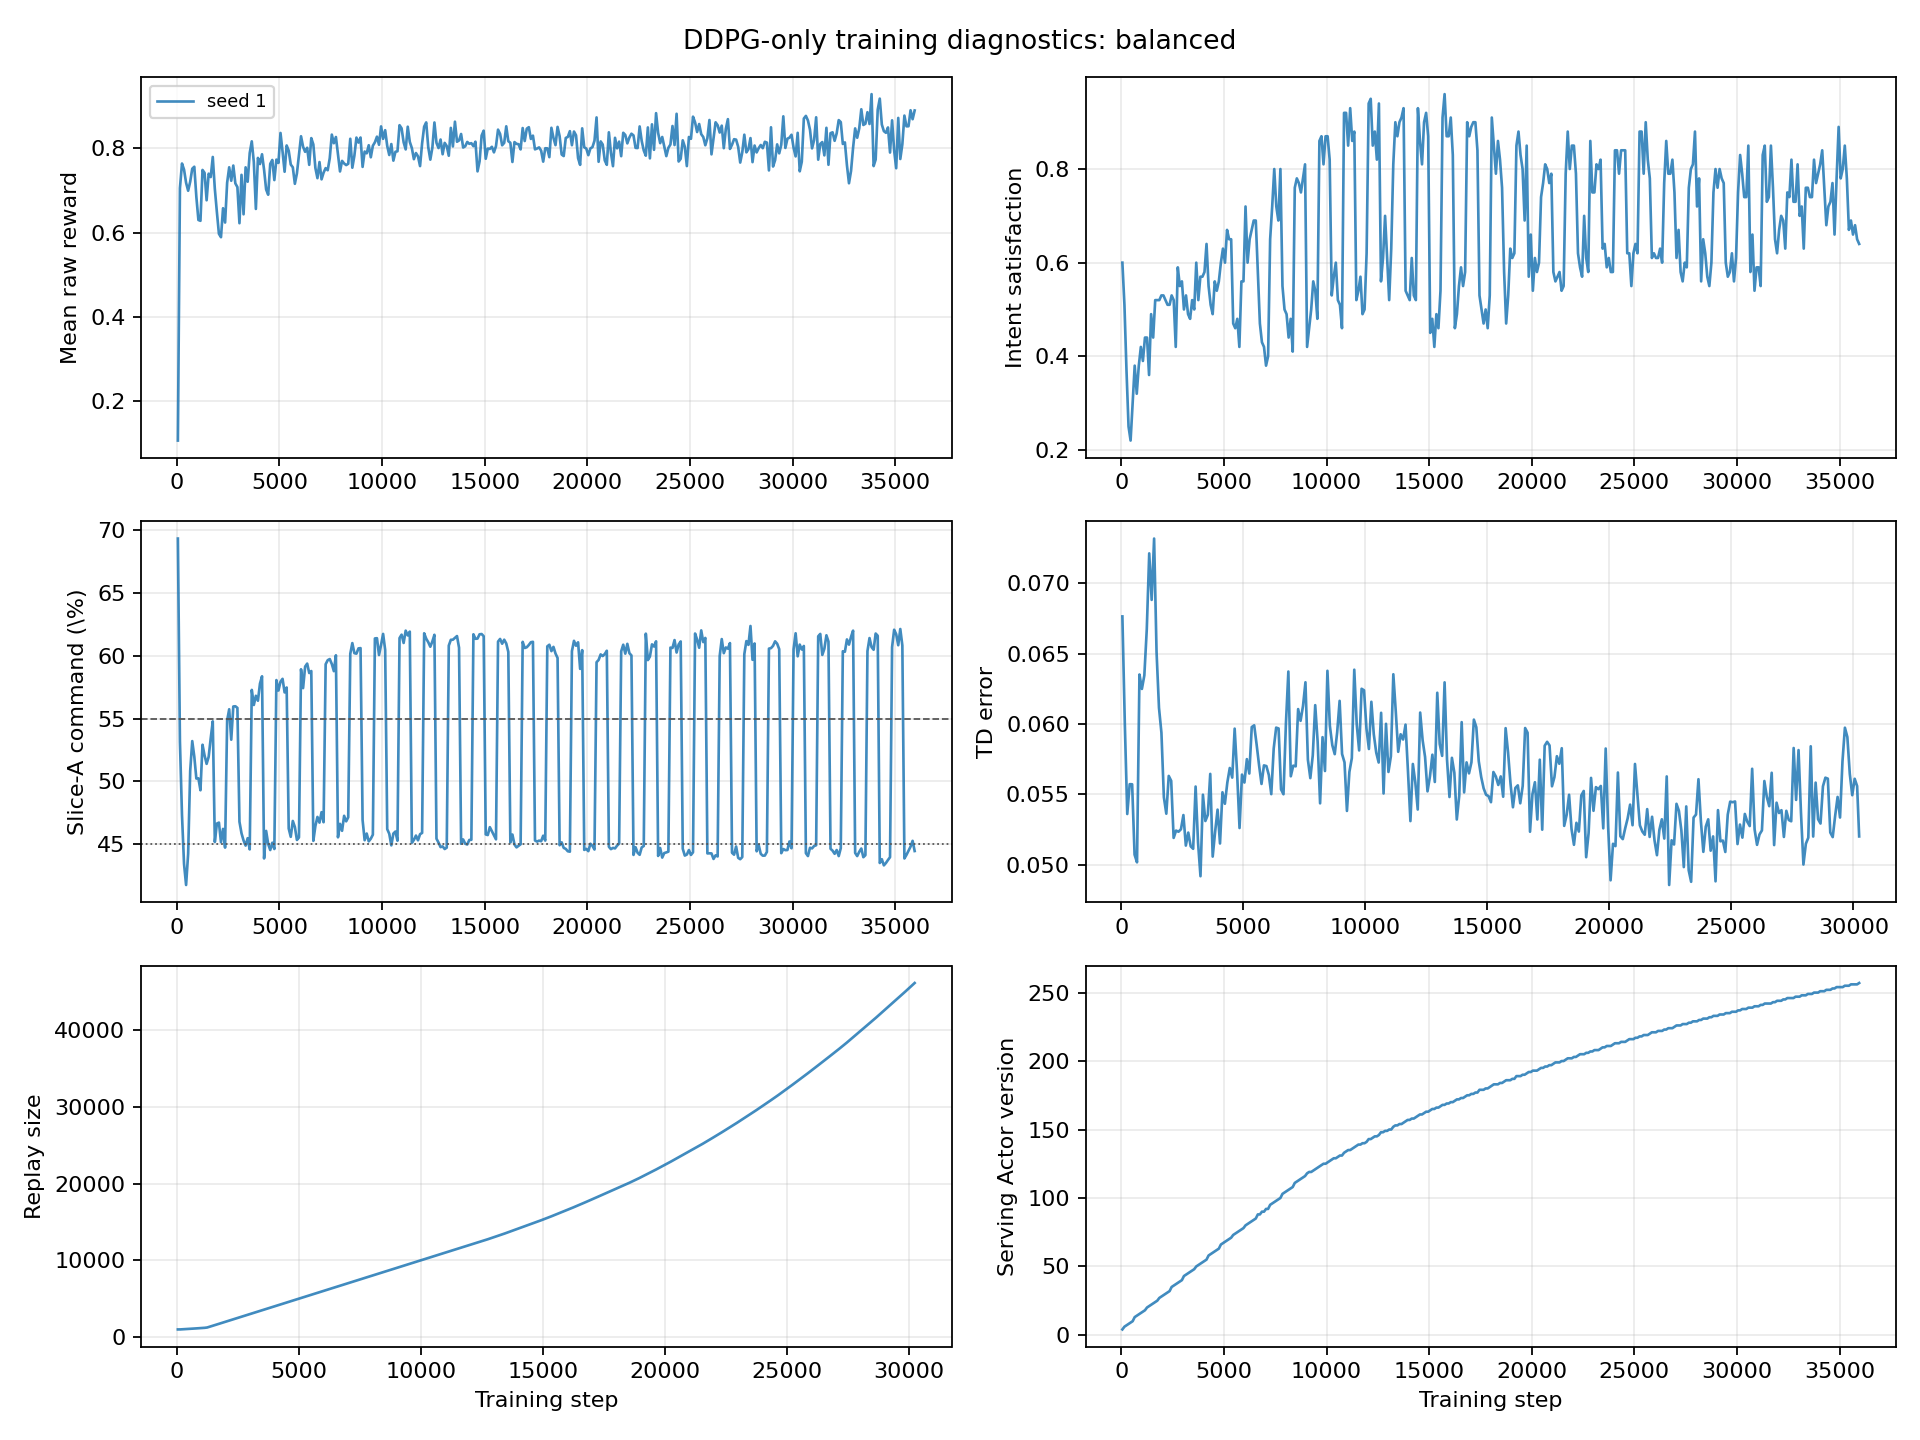
\includegraphics[width=0.94\textwidth]{generated/balanced_ddpg_only_diagnostics.png}}{\fbox{Generate results to create the DDPG-only diagnostics.}}
  \caption{DDPG-only training diagnostics. Curves are aggregated into 100-transition bins; the single-seed pilot is shown without a confidence envelope. The two dashed Slice-A levels indicate the 55\% A-priority and equivalent 45\% B-priority command thresholds.}
  \label{fig:ddpg-only-learning}
\end{figure*}

\begin{figure}[t]
  \centering
  \IfFileExists{generated/balanced_performance_comparison.png}{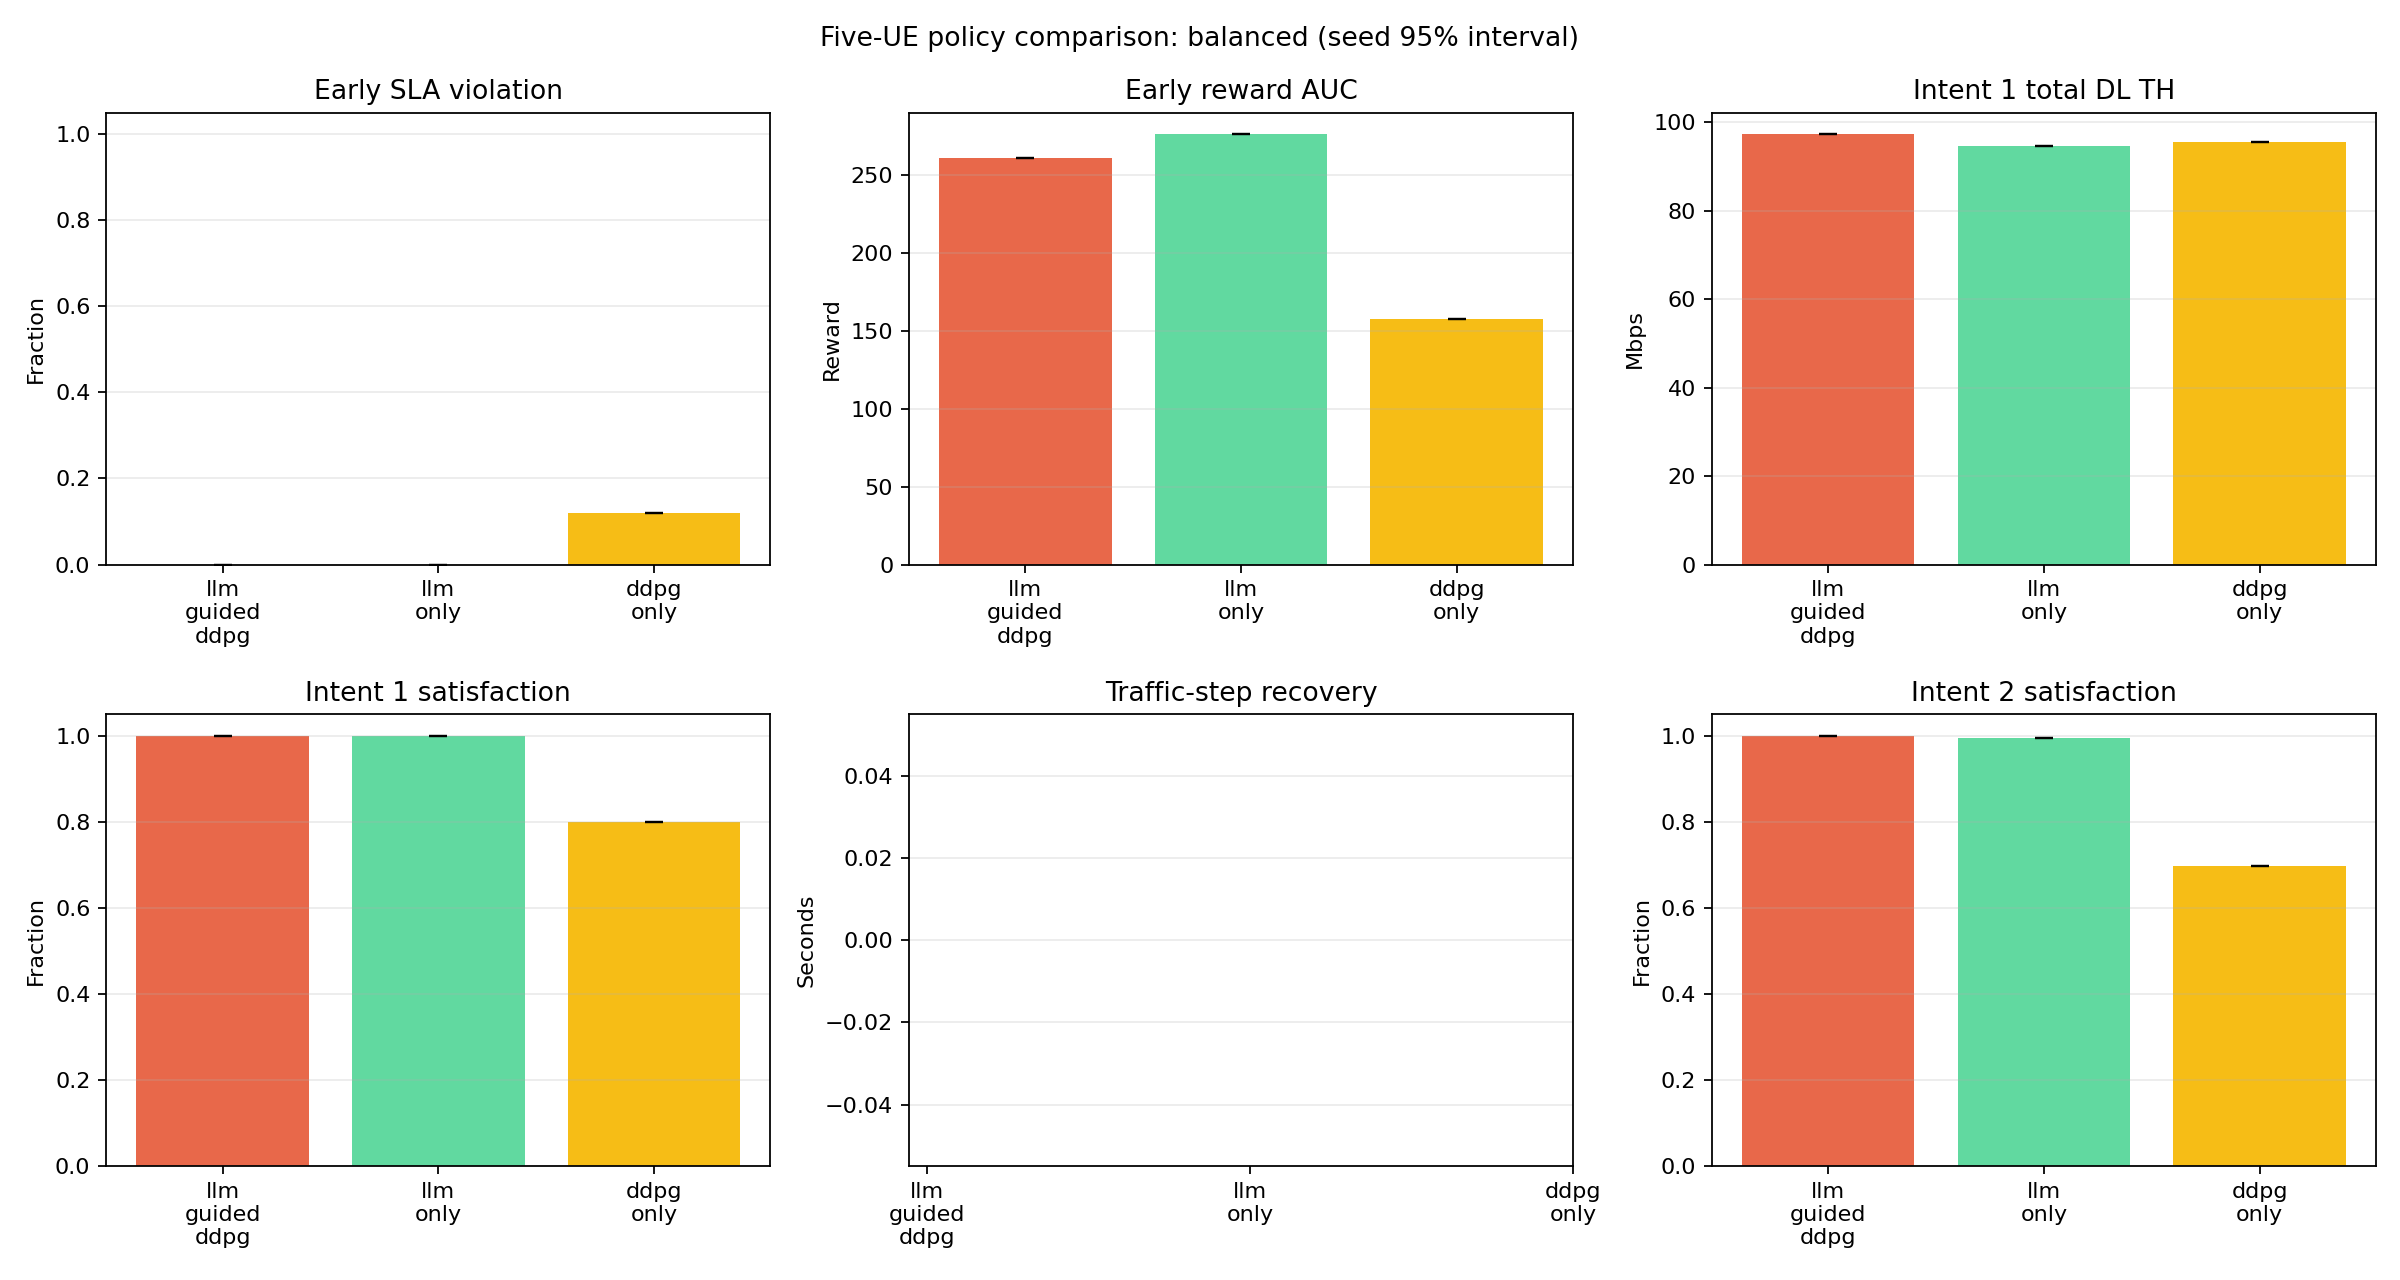
\includegraphics[width=\columnwidth]{generated/balanced_performance_comparison.png}}{\fbox{Generate results to create this figure.}}
  \caption{Balanced seed-1 performance comparison. Confidence intervals are intentionally omitted for the single-seed pilot.}
  \label{fig:pilot-performance}
\end{figure}
\FloatBarrier

\subsection{Learning behavior}
Each learning arm logged the full 40{,}600 protocol control steps of the four validated phases
and inserted about $4.6\times10^4$ transitions into the asynchronous replay --- 45{,}726 for
guided control and 46{,}317 for the unguided arm --- the surplus over the 1{,}000 prefilled
calibration and 36{,}000 training transitions being uncounted intent-switch steps. Every
inserted transition passed the per-transition trainability test in every phase. The learner
performed 30{,}207 and 30{,}266 updates at 6.57 and 6.54~Hz, of which 15{,}103 and 15{,}133
were Actor updates because of the delayed-update interval of two. Replay rows reached the
learner with a mean insertion age of 1.74~s (guided) and 1.65~s (unguided) at mean queue
depths of about 2{,}900 and 3{,}000 rows, which quantifies the decoupling between the 100~ms
control loop and the learner; Fig.~\ref{fig:learning} plots the resulting learner diagnostics.

Candidate publication behavior differed sharply. Both learning arms produced 257 candidate
Actors, but the guided run accepted 62 and rejected 195, whereas the unguided run accepted all
257. The accepted count for the guided run is an upper bound on genuine quality-gate passes:
the learner implements a force-promotion escape hatch that publishes a gate-failing candidate
after six consecutive rejections, provided it is finite and projects legally into the active
bounds, and the per-candidate accepted/forced split was recorded only in the run databases,
which are lost, so the split cannot now be recovered for this pilot. The
serving path diverged further from the candidate stream: the controller observed 61 distinct
serving Actor versions and performed 50 atomic swaps in the guided run, against 244 versions
and 204 swaps in the unguided run, with a maximum swap cost below 0.7~ms in both. The
distinction between candidate records, accepted versions, and actually served versions is
preserved in the artifact.

\begin{figure}[t]
  \centering
  \IfFileExists{generated/balanced_ddpg_learning.png}{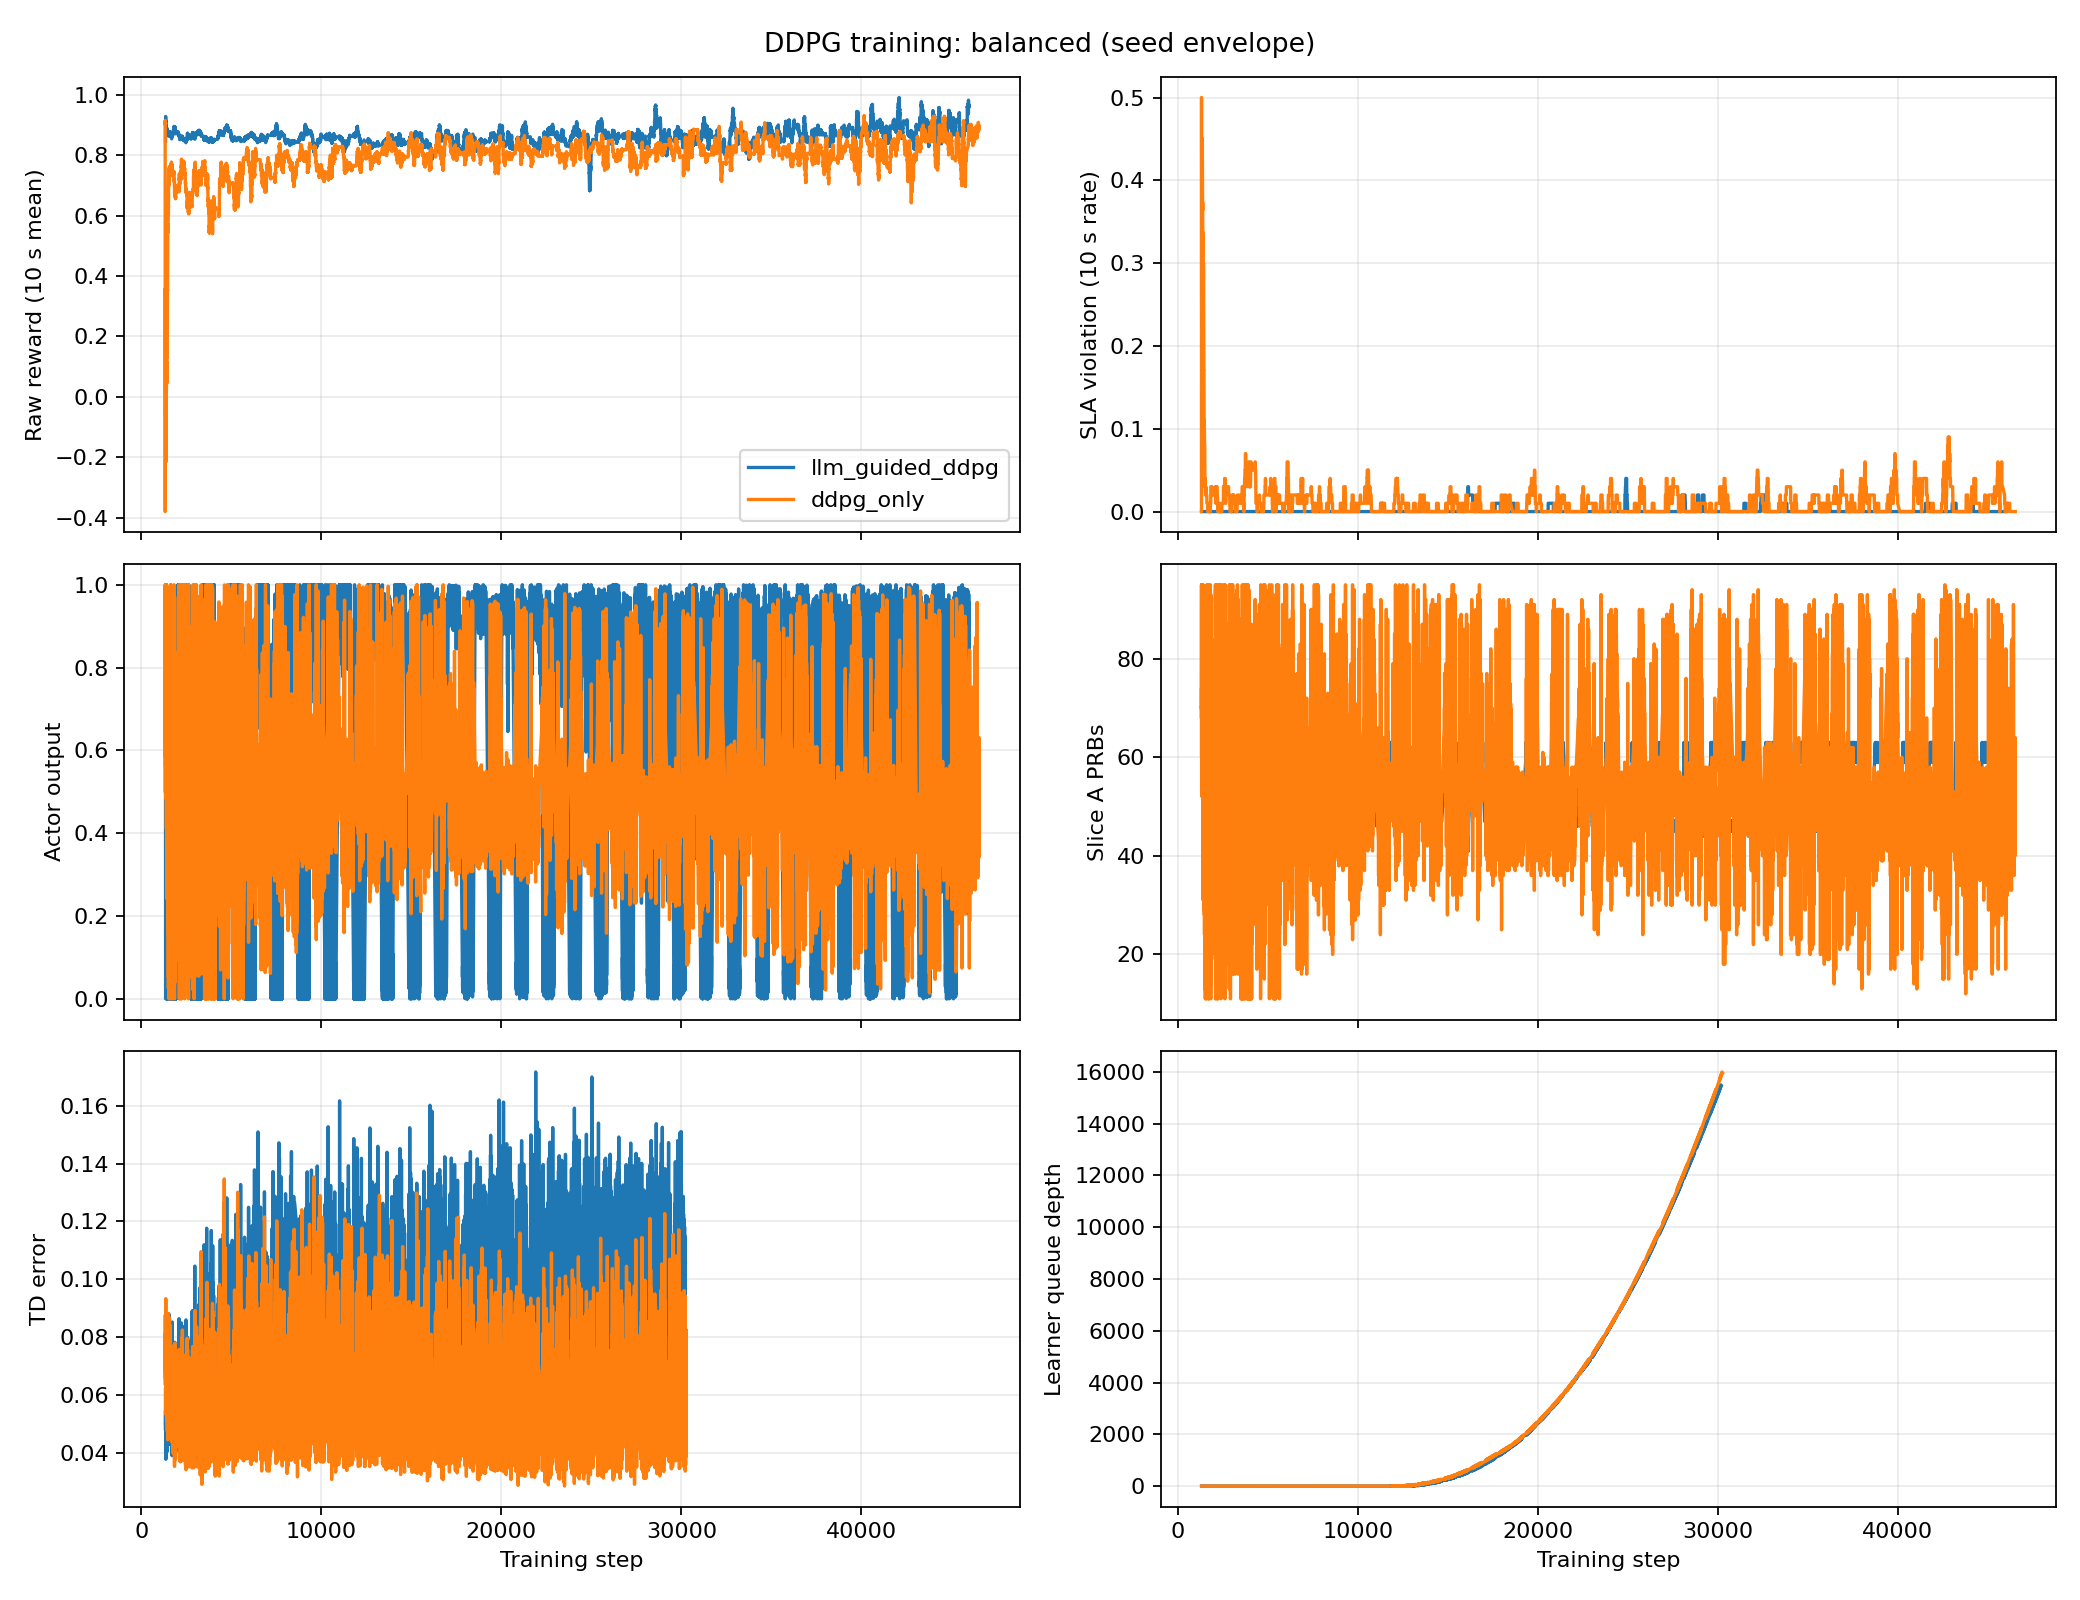
\includegraphics[width=\columnwidth]{generated/balanced_ddpg_learning.png}}{\fbox{Generate results to create this figure.}}
  \caption{Learning diagnostics generated from raw experiment and learner tables.}
  \label{fig:learning}
\end{figure}

The UDP offered load intentionally saturates the radio. Against 30~Mbps offered per UE, the
mean delivered rate at the UE TUN interface was 17.8--18.4~Mbps, i.e.\ 38.8--40.5\%
offered-versus-delivered downlink loss across the three arms. This figure is computed from
receiver byte counters against the nominal offered rate; it is not the iperf3 sender's own
datagram-loss report, and it is therefore not a control failure but the expected consequence
of running the cell in overload so that the PRB ratio is the binding constraint. We
consequently keep receiver goodput and RLC-derived throughput as separate quantities
throughout. All three arms recorded the same traffic trace hash, confirming that they were
offered identical load. The dynamic heavy-load scenarios, in which the 5~s phase pattern is
imposed by the HTB shaper of Section~\ref{sec:methodology}, are
required to assess response to demand shifts and remain placeholders until complete primary
runs are available; because the balanced pilot never installs the shaper, its 100\% segment
success rate carries no information about shaper fidelity.

\ifFullCampaign\else
The full 3-scenario, 3-arm, 5-seed campaign is incomplete. No paired-bootstrap interval or
cross-scenario claim is reported in this version, and no statement in this section should be
read as a statistical comparison: every value above comes from one seed of one scenario.
\fi
\FloatBarrier

\section{Standards Boundary and Limitations}
\label{sec:limitations}
This section states precisely what is standards-aligned, what is prototype-specific, and what the reported evidence does and does not support. It is deliberately detailed: an implementation appendix is only useful if its deviations are enumerated.

\subsection{What follows the standards}
S-NSSAI, DNN, registration, and PDU-session procedures use the existing 3GPP mechanisms~\cite{3gpp23501}; no NAS, NGAP, RRC, or PHY message is redefined, and the S-NSSAI that the scheduler matches on is the one the core signalled for the UE's data radio bearer. The E2 path uses E2AP~v2 with the FlexRIC E2SM-RC service model (short name \texttt{ORAN-E2SM-RC}, OID \texttt{1.3.6.1.4.1.53148.1.1.2.3}) and ASN.1/PER encoding, and the added control reuses that stock encoder unmodified. The control message reproduces the E2SM-RC RRM Policy Ratio List parameter hierarchy with the standard RAN parameter identifiers. E2SM-KPM~v2.03 measurements are collected on a separate, unmodified subscription and kept as an audit record.

\subsection{Prototype-specific deviations}
The system is a research prototype, not a certified O-RAN product, and the following deviations are known and intentional.
\begin{itemize}
  \item Control Service Style~2, Action~6 (\emph{Slice-level PRB quota}) is added locally to the OAI RC RAN function. Its semantics have not undergone O-RAN conformance testing.
  \item SST and SD are transported as ASCII-text octet strings (or plain integers) rather than the 3GPP binary octet encoding, and an absent SD is defaulted to \texttt{0xffffff} by the decoder.
  \item The PLMN Identity element is required to be present in each RRM Policy Member but is never read or checked by the gNB; policy matching uses only SST and SD.
  \item The RIC Control Acknowledge is returned with a success outcome even when the gNB rejects the message. A rejection is observable only as an assertion trace and an error line in the gNB log, so a controller cannot distinguish ``applied'' from ``parsed but refused'' over E2. The measured acknowledgement rate reported in the results therefore certifies the E2 round trip, not the RAN-side acceptance.
  \item The policy service that carries intent and guidance is \emph{A1-like}: it fills the policy role this prototype needs, with versioned atomic activation, but it is not an O-RAN A1-PMS implementation~\cite{oran_a1}.
  \item The rich near-RT state is derived from FlexRIC internal service models, not from E2SM-KPM. KPM is an independent audit path and must not be presented as the source of every state feature.
  \item The core profile has slice-aware subscriber, DNN, AMF, and SMF configuration but no separately deployed NSSF. RNTI-to-UE-to-S-NSSAI attribution is reconstructed from runtime logs and configuration with an explicit validity mask; a production deployment should use a standardized identity-correlation path.
  \item One change is unrelated to the system and exists purely so the reference testbed builds: the RFSimulator option table was rewritten from designated-initializer macros to small by-value constructor helpers, because the file is compiled as C++ and the macros are rejected by the reference GCC~10 toolchain. Parameter names, defaults, and semantics are unchanged. Omitting this change makes the reproduction instructions fail.
\end{itemize}

\subsection{Scheduler limitations}
The dedicated ratio is enforced as a per-slot budget on \emph{new-data} allocation only, computed as $\lfloor n_{\mathrm{rb,avail}}\cdot r_{\mathrm{dedicated}}/100\rfloor$ over the full cell bandwidth. Several consequences follow and bound the generality of the results.
\begin{itemize}
  \item HARQ retransmissions and the small allocations for timing-advance or beam-switch control elements are served before any slice budget and are not charged against it. Slice quotas can therefore never suppress retransmissions, but retransmission PRBs do reduce the free blocks the budgeted pass can subsequently find, so the realized share can fall below the commanded share under heavy retransmission.
  \item Minimum and maximum ratios are validated at the E2 boundary but are not independent scheduler mechanisms; only the dedicated ratio is enforced, and bound projection is performed by the near-RT controller before transmission.
  \item Unused budget of one controlled slice is not lent to another controlled slice. Saturating traffic on both slices is therefore a precondition for the commanded ratio to be observable, which is why the campaign offers 150~Mbps against a cell that cannot carry it.
  \item Each UE's budgeted allocation is a single largest contiguous free block, capped by the remaining budget. Fragmentation can leave part of a slice budget unusable within a slot.
  \item A slice whose dedicated ratio is zero is skipped by its own pass and is excluded from the unmatched pass as well, so a zero dedicated ratio yields zero new-data PRBs rather than best-effort service. The operational 10\% floor prevents this in the campaign.
  \item Matching is exact on the pair (SST, SD): there is no wildcard or partial match, and a UE with no data radio bearer defaults to SST~0 / SD \texttt{0xffffff} and matches nothing. For a UE with several bearers on different slices the candidate takes the S-NSSAI of the first bearer reporting a non-zero 5QI; this is unambiguous here because every UE has exactly one PDU session and one bearer.
  \item The per-slice budget sums the available resource blocks over all beams while the allocation hook is invoked once per beam group. This is exact only for a single beam, which is the configuration used.
  \item Independently of any policy, the downlink control-channel budget limits the testbed to at most four scheduled UEs per downlink slot out of five, so no PRB policy can serve all five UEs in the same slot.
  \item The policy installer clears the table before re-validating each entry and does not restore the previous table if an entry is rejected mid-loop. This is unreachable in the deployed path because the E2 decoder applies identical bounds first and installs nothing on failure, but it is a latent fault for any other caller.
\end{itemize}
Results therefore characterize this implementation, not all possible slicing schedulers.

\subsection{Measurement limitations}
Two reported quantities are weaker than they appear. Under the static AWGN RFSimulator profile used for the pilot, the MAC block-error-rate and wideband-CQI counters are effectively unpopulated: their run means are $5.6\times10^{-45}$ and $0.0$ respectively across all three runs. They must not be cited as measured radio quality, and the BLER term of the reward is consequently inert in this pilot, so its weight is untested. Second, the reported downlink loss is an offered-versus-delivered ratio computed from the UE tunnel-interface byte counters against the nominal offered rate; it is not the sender's own datagram-loss report, and it should not be read as a control failure under an intentionally saturating offered load.

\subsection{Control-loop and learning limitations}
\begin{itemize}
  \item \emph{Guidance acted mainly as a constraint.} In the pilot, 90.66\% of guided training actions and 92.1\%/78.2\% of its two evaluation phases sat within half a PRB of an edge of the active feasible interval, against 0.34\%/0\%/0\% for the unguided arm. Because the Intent-1 guidance floor of 55\% maps to $b_A\geq 59$ and the guided evaluation mean was 59.27 PRBs, the guided policy was effectively pinned to the guidance boundary rather than exploring inside it. The guided arm's advantage in this run should therefore be attributed primarily to the calibrated constraint, not to a richer learned policy.
  \item \emph{Accepted-Actor counts are an upper bound.} The learner contains a force-promotion escape hatch that publishes a finite, legally projected candidate after six consecutive holdout rejections. With 195 rejections among 257 candidates in the guided run, the reported 62 acceptances is an upper bound on the number that passed the quality gates outright; the accepted-versus-forced split lives only in the run databases.
  \item \emph{Evaluation is not fully frozen.} Freezing suspends the Actor, replay ingestion, and the observation normalization statistics, but the guidance-fusion weight and the intent-violation fallback counters continue to update during evaluation.
  \item \emph{The two learning arms do not bootstrap over identical episodes.} A transition is marked terminal when its governing policy version changes. For the guided arm that is the A1 policy version, renewed every 10~s; for the unguided arm it is the intent version, renewed only at an intent switch. The guided arm therefore learns over markedly shorter effective episodes, which is a confound in any guided-versus-unguided comparison.
  \item \emph{One logged column is inert.} In asynchronous mode the controller-side reward scaler is never updated and is not shipped in the Actor snapshot, so the recorded running standard deviation is identically unity and the recorded scaled reward equals the raw reward. Reward scaling is performed inside the learner; the controller-side columns are an audit copy at unit scale.
\end{itemize}

\subsection{Evidence and reproducibility limitations}
The pilot is a single balanced-load seed. It cannot separate policy effects from seed-specific training and runtime variation, and no statistical claim is made from it. Beyond that, five reproducibility caveats should be recorded honestly.

First, the three run databases referenced by the artifact manifest, of 1.0--1.3~GB each, together with every trained checkpoint, were written under \texttt{/tmp} and were destroyed when the host was rebooted to repair an unrelated GPU driver fault, because that directory does not survive a reboot. Every number in this paper was re-verified against the committed comma-separated metric files and against the code that produces them, but the pilot is currently reproducible from code and protocol rather than re-derivable from raw data. Run databases must be archived outside \texttt{/tmp} before any campaign is considered complete.

Second, database freshness and the RAN/RIC restart are conditional on invoking the runner with its stack-management flag; without it, runs append to a single shared database and the mapped-UE validation query, which carries no run or time filter, counts UEs across the entire file. All campaign runs must use that flag.

Third, the result generator keys runs on the tuple (scenario, arm, seed) and does not consult the manifest mode field. A checkpoint-evaluation run validates against a reduced phase set, can legitimately reach primary quality, and---being newer---would supersede the corresponding full training run, silently removing its training phase from the tables. No claim of checkpoint-evaluation isolation is made here; until the generator is fixed, checkpoint evaluations must be written to a separate results directory.

Fourth, two thresholds present in the campaign specification are recorded but never enforced: the 99th-percentile fresh-action-interval bound and the maximum summary age. Conversely, the enforced control-latency and effect-coverage bounds are hard-coded in the runner rather than specification-driven. The set of gates actually applied is the one enumerated in the methodology section, not the full key list of the specification file.

Fifth, seeding covers the Python and PyTorch generators in both the controller and the learner process and derives the channel-trace seeds, and arm order within each seed and scenario is shuffled deterministically; but NumPy, CUDA, and cuDNN determinism are not forced, and the learner advances on wall clock. Runs are therefore statistically, not bitwise, reproducible. The cost is also material: a single run takes 85--88~minutes against a 4090~s nominal phase budget, the roughly 27\% overhead being A1 guidance regeneration across the 64 intent switches, so the full 45-run campaign requires on the order of 65~hours of continuous testbed time.

Finally, the scope of the radio experiment itself is narrow: one gNB, static AWGN, RFSimulator, local network namespaces, downlink-only control, and two slices. Commercial RU operation would additionally require timing synchronization, RF calibration, DU/RU integration, and renewed real-time validation.

\section{Conclusion}
This appendix documented the extension of the \systemname{} framework~\cite{bao2026llmhric} from simulated IAB power allocation to per-S-NSSAI downlink PRB allocation on a running OAI/FlexRIC system, and the implementation and deployment work that extension required. Concretely: an E2SM-RC Style~2 / Action~6 control path and an S-NSSAI-aware downlink allocator were added to OAI; a persistent RC xApp actuates every 100~ms without opening an E2 association per action; 50~ms slice summaries with explicit identity and provenance masks supply the near-RT state; a locally hosted quantized Gemma rApp publishes intent-conditioned targets every 10~s through an A1-like versioned policy service, projected into calibration-derived bounds; and a TD3-style actor--critic learns asynchronously from acknowledged actions and their measured effects, entering the control loop only through validated, atomically swapped Actor snapshots.

\ifFullCampaign
The complete three-scenario, three-arm, five-seed campaign is reported with same-seed paired intervals.
\else
The evidence released with this version is a balanced-load, single-seed pilot of three runs. It shows that the loop closes and is instrumented end to end---all controls acknowledged, five UEs mapped throughout, full effect-window coverage, and every logged transition admissible for learning---and it shows encouraging differences in intent satisfaction and aggregate throughput. It does not establish statistical superiority of any arm, and this paper makes no such claim. The pilot also exposes a specific weakness to address before the full campaign: the guided policy sat on the guidance boundary for the large majority of its actions, so guidance functioned largely as a calibrated constraint rather than as a learning signal.
\fi

What is released is the derived evidence rather than the measurements themselves: the full source and OAI/FlexRIC patches, the campaign specification and validation gates, the result-generation scripts, and, for each executed run, the derived metrics, the generated tables and figures, and a manifest pinning the specification digest and the code revisions. The raw run databases and the trained checkpoints of the pilot were lost and cannot be re-analysed, so every reported number is traceable to the released derived metrics but none can be re-derived from raw data (Section~\ref{sec:limitations}). The remaining work is accordingly to re-run the 45-run campaign with its databases archived on persistent storage, to close the result-generator and validation gaps identified in Section~\ref{sec:limitations}, and to replace every pilot statement with paired multi-scenario estimates. The artifact is available at \codeurlprinted.


\bibliographystyle{IEEEtran}
\bibliography{references}
\end{document}
